\section{Expanded Algorithm and Guarantee Statements}
\label{app:expanded-guarantees}


\begin{definition}[Iteration and ablation]
For $p_t=(B_t,A_t)$, $\beta\in[0,1)$, $\eta_t>0$, let
\begin{align}
(\bar B_t,\bar A_t)&={\rm Bal}(B_t,A_t)
=(B_tQ_t,Q_t^{-1}A_t),\\
H_t&=\bar B_t^\top\bar B_t=\bar A_t\bar A_t^\top,\\
\widetilde M_{B,t-1}&=M_{B,t-1}Q_t,\\
\widetilde M_{A,t-1}&=Q_t^{-1}M_{A,t-1},\\
g_{B,t}&=\nabla f_{I_t}(X_t)\bar A_t^\top,\\
g_{A,t}&=\bar B_t^\top\nabla f_{I_t}(X_t),\\
U_{B,t}&=\beta\widetilde M_{B,t-1}+(1-\beta)g_{B,t},\\
U_{A,t}&=\beta\widetilde M_{A,t-1}+(1-\beta)g_{A,t},\\
C_t&=\bar B_t^\top U_{B,t}-U_{A,t}\bar A_t^\top,\\
H_{\varepsilon,t}&=H_t+\varepsilon I,\\
H_{\varepsilon,t}\Omega_t+\Omega_tH_{\varepsilon,t}&=C_t,\\
M_{B,t}&=U_{B,t}-\bar B_t\Omega_t,\\
M_{A,t}&=U_{A,t}+\Omega_t\bar A_t,\\
B_{t+1}&=\bar B_t-\eta_tM_{B,t},\\
A_{t+1}&=\bar A_t-\eta_tM_{A,t}.
\label{eq:main-iteration}
\end{align}
The balance-only ablation sets $(M_{B,t},M_{A,t})=(U_{B,t},U_{A,t})$.
The analyzed first-moment iteration is distinct from an elementwise
second-moment adaptive heuristic.
\end{definition}

The proof uses the second-order pullback-Hessian theorem
\citep[Proposition 5.45]{boumal2023introduction} to combine the connection
terms exactly. Schur modal analysis and a discrete Lyapunov certificate
then control the actual momentum state. For statistics, whitening
precedes the Laurent--Massart quadratic-form bound, and the resulting
leading constant is compared with Fisher information.

\begin{theorem}[Quotient metric, stationarity, and finite-step decomposition]
For $X=U\Sigma V^\top\in\mathcal K_{a,b}$,
\begin{align}
K_X(G)&=U\Sigma U^\top G+GV\Sigma V^\top,&
g_X(Z,Y)&=\ii Z{K_X^\dagger Y},\\
\qgrad_g f(X)&=K_X(\nabla f(X)),&
(2b)^{-1}\nn Z^2&\leq\gn Z^2\leq a^{-1}\nn Z^2,\\
\bar B^\top g_B-g_A\bar A^\top&=0 .
\end{align}
For $u=h+(\bar B\Omega,-\Omega\bar A)$,
\begin{equation}
X_{\rm unproj}^+-X_{\rm proj}^+
=\eta^2(-h_B\Omega\bar A+\bar B\Omega h_A-\bar B\Omega^2\bar A).
\label{eq:main-cross}
\end{equation}
For a unit horizontal lift $\xi$ and $G=\nabla f(X)$,
\begin{align}
{\rm Hess}_g f[L_p\xi,L_p\xi]
&=\ii{L_p\xi}{\nabla^2 f[L_p\xi]}+2\ii G{\xi_B\xi_A},\\
\|\qHess_g f(X)\|_{g\to g}
&\leq 2b\|\nabla^2 f(X)\|_{F\to F}+\|G\|_2 .
\end{align}
The residual coefficient one is attained
(Appendix~\ref{app:sharp-pullback}).
At a nondegenerate quotient critical point the full factor Hessian has
exactly $r^2$ gauge zero directions. Complete derivations are in
Appendices~\ref{app:geometry}--\ref{app:rigid-calculus}.
\end{theorem}

\begin{theorem}[Stochastic and momentum convergence]
Under the regularity, pullback, oracle, and stepsize assumptions in
Appendix~\ref{app:convergence}, a biased quotient-gradient update satisfies
\begin{equation}
\frac{\sum_{t<T}\eta_t\E\gn{g_t}^2}{S_T}
\leq\frac{2\Delta_0+
4\sum_{t<T}\eta_t\E\gn{b_t}^2+
L_R\sum_{t<T}\eta_t^2\nu_t^2}{S_T},
\quad S_T=\sum_{t<T}\eta_t .
\label{eq:main-convergence}
\end{equation}
For transported normalized momentum satisfying
Eq.~\eqref{eq:rigid-momentum-step},
\begin{equation}
\frac1T\sum_{t<T}\E\gn{g_t}^2
\leq\frac{2\Delta_0}{\eta T}
+\frac{2q_0}{(1-\beta)T}+2(1-\beta)\nu^2 .
\end{equation}
For noiseless RIP sensing in an invariant geodesically convex basin
with $k_-(X)\geq a$ and
$\|X-X_*\|_2+\delta\|X-X_*\|_F\leq\omega<a(1-\delta)$,
\begin{align}
\mu_{\rm RIP}&=a(1-\delta)-\omega,&
f(X_T)&\leq(1-\eta\mu_{\rm RIP})^Tf(X_0).
\end{align}
The noisy, high-probability, numerical-error, and admissible-basin
statements are proved separately in Appendix~\ref{app:convergence}.
\end{theorem}

\begin{theorem}[Joint deep-chain spectrum]
For the canonical balanced depth-$L$ chain, its joint vertical normal
operator has eigenvalues
\begin{align}
\lambda_{abk}
&=\sigma_a^{2/L}+\sigma_b^{2/L}
-2(\sigma_a\sigma_b)^{1/L}\cos(k\pi/L),\\
\kappa(\mathcal V_W^*\mathcal V_W)
&=\kappa(X)^{2/L}\cot^2(\pi/(2L)).
\end{align}
Its product preconditioner has core eigenvalues
\begin{equation}
\chi_{ab}^{(L)}
=\sum_{i=1}^L\sigma_a^{2(L-i)/L}\sigma_b^{2(i-1)/L}.
\end{equation}
The normal solve and product-optimization spectra are different objects.
Appendix~\ref{app:rigid-chain} gives diagonalization, damping error,
complexity, and aligned-mode hitting-time proofs.
\end{theorem}


\begin{theorem}[Sharp local momentum factor]
At a regular quotient minimum with Hessian spectrum in $[\mu,\Lambda]$,
the reduced position--memory Jacobian has characteristic polynomials
\begin{equation}
z^2-\{1+\beta-\eta(1-\beta)\lambda\}z+\beta,\quad
\lambda\in\operatorname{spec}(\qHess_g f).
\end{equation}
Its exact stability condition and optimal interval-wide factor are
\begin{align}
0<\eta(1-\beta)\Lambda&<2(1+\beta),\\
q_\star&=\frac{\sqrt\Lambda-\sqrt\mu}{\sqrt\Lambda+\sqrt\mu},&
\beta_\star&=q_\star^2,&\eta_\star&=(\mu\Lambda)^{-1/2}.
\end{align}
A discrete Lyapunov equation gives the invariant nonlinear contraction
ball in Eq.~\eqref{eq:local-certified-radius}.
For Frobenius reconstruction at the best rank-$r$ approximation to $Y$,
with a strict retained/omitted singular-value gap and a nonempty
off-core tangent block,
\begin{equation}
\mu=\sigma_r(Y)-\sigma_{r+1}(Y),\qquad
\Lambda=2\sigma_1(Y).
\end{equation}
These extrema follow from the complete spectrum
$\{\sigma_i+\sigma_j,\sigma_i\pm\tau_k,\sigma_i\}$ in
Appendix~\ref{app:local-dynamics}.
\end{theorem}

\begin{theorem}[Statistical guarantees under declared sampling assumptions]
For adjacent IID datasets and the actual state-map regularity in
Eq.~\eqref{eq:rigid-state-regularity},
\begin{equation}
\epsilon_{\rm stab}\leq
\frac{2C_\ell C_U}{n}\sum_{t<T}\eta_t
\prod_{k>t}(1+L_U\eta_k).
\label{eq:main-generalization}
\end{equation}
For a bounded product class and empirical suboptimality
$\epsilon_{\rm opt}$,
\begin{align}
R(X_T)-\inf_{\mathcal C}R
&\leq\epsilon_{\rm opt}+2U_n,\\
\E R(X_T)-\inf_{\mathcal C}R
&\leq\epsilon_{\rm opt}+\epsilon_{\rm stab}.
\end{align}
Here $U_n$ may be the nuclear-norm, intrinsic-chart, network, or margin
bound in Appendix~\ref{app:generalization}. A squared-gradient guarantee
alone does not supply $\epsilon_{\rm opt}$.
\end{theorem}

\begin{theorem}[Whitened local risk and its efficiency constant]
Under the relative-Hessian, score-tail, and localization conditions of
Appendix~\ref{app:sharp-statistics}, with probability at least
$1-q_H-e^{-u}$,
\begin{equation}
R(\widehat X_n)-R(X_\star)
\leq\frac{1+\epsilon_H}{2n(1-\delta_H)^2}
\{\operatorname{tr}\mathsf V+
2\sqrt{\operatorname{tr}(\mathsf V^2)u}+2\|\mathsf V\|_2u\}.
\end{equation}
For a correctly specified identifiable sensing model with homoscedastic noise variance
$\sigma_\varepsilon^2$, the local influence and averaging results give,
under their stated expectation conditions,
\begin{equation}
n\,\E[R(\widehat X_n)-R(X_\star)]
\longrightarrow\frac{\sigma_\varepsilon^2}{2}r(m+d-r).
\end{equation}
The same constant is the Cram\'er--Rao lower bound for locally unbiased
estimators under quadratic tangent loss. The finite-sample coefficient
$1/2$ is an equality for a quadratic chart model with exact reference
Hessian (Appendix~\ref{app:local-statistics}).
\end{theorem}

\section{Regular Quotients, Balanced Lifts, and Exact Finite-Step Identities}
\label{app:geometry}
\subsection{Spaces, actions, and local coordinates}
\begin{definition}
\begin{align}
1\leq r&\leq\min(m,d),\qquad 0<a\leq b<\infty,\\
\mathcal P&=\R_*^{m\times r}\times\R_*^{r\times d},\\
\pi(B,A)&=BA,\\
\Phi_Q(B,A)&=(BQ,Q^{-1}A),\qquad Q\in{\rm GL}(r),\\
\mathcal M_r&=\{X:\rnk X=r\},\qquad
\mathcal Q=\mathcal P/{\rm GL}(r),\\
\mathcal S&=\{(B,A)\in\mathcal P:B^\top B=AA^\top\},\\
\mathcal K_{a,b}&=\{X\in\mathcal M_r:a\leq\sigma_r(X),\
\sigma_1(X)\leq b\}.
\label{eq:rigid-domain}
\end{align}
The two starred factor spaces have full column and row rank, respectively.
\end{definition}

\begin{theorem}[Principal quotient and product identification]
\label{thm:quotient-space}
\begin{align}
\pi(p)=\pi(p')&\iff\exists!Q\in{\rm GL}(r):p'=\Phi_Q(p),\\
\mathcal Q&\simeq\mathcal M_r,&
\dim\mathcal Q&=r(m+d-r),\\
D\pi_p[\xi]&=\xi_BA+B\xi_A,&
\ker D\pi_p&=\{(B\Omega,-\Omega A):\Omega\in\R^{r\times r}\}.
\label{eq:rigid-kernel}
\end{align}
The action is free and proper.
\end{theorem}
\begin{proof}
\begin{align}
BA=B'A'&\Longrightarrow\qrange B=\qrange B'
\Longrightarrow B'=BQ,\quad Q=B^\dagger B'\in{\rm GL}(r),\\
BA=BQA'&\Longrightarrow A=QA'\Longrightarrow A'=Q^{-1}A,\\
BQ=B&\Longrightarrow Q=B^\dagger B=I_r.
\end{align}
For $p_k\to p\in\mathcal P$ and $\Phi_{Q_k}p_k\to p'\in\mathcal P$,
\begin{align}
Q_k&=B_k^\dagger B_k'\to B^\dagger B',\\
Q_k^{-1}&=(B_k')^\dagger B_k\to(B')^\dagger B,&
(B^\dagger B')((B')^\dagger B)&=I_r.
\end{align}
For $|I|=|J|=r$ and $\det X_{I,J}\ne0$,
\begin{align}
s_{I,J}(X)&=(X_{:,J},X_{I,J}^{-1}X_{I,:}),&
\pi(s_{I,J}(X))&=X.
\label{eq:pivot-section}
\end{align}
These maps give smooth local inverse quotient maps. Furthermore,
\begin{align}
D\pi_p[\xi]=0
&\Longrightarrow(I-BB^\dagger)\xi_BA=0\\
&\Longrightarrow\xi_B=B\Omega,\quad\Omega=B^\dagger\xi_B\\
&\Longrightarrow B(\Omega A+\xi_A)=0
\Longrightarrow\xi_A=-\Omega A,\\
\dim\mathcal Q&=mr+rd-r^2.
\end{align}
\end{proof}

\begin{proposition}[Explicit regular rank chart]
\label{prop:schur-chart}
Fix $X=U\Sigma V^\top$ and orthogonal completions $U_\perp,V_\perp$.
For $C\in{\rm GL}(r)$,
$D\in\R^{r\times(d-r)}$, $E\in\R^{(m-r)\times r}$,
\begin{equation}
\Psi(C,D,E)=[U,U_\perp]
\begin{pmatrix}C&D\\E&EC^{-1}D\end{pmatrix}[V,V_\perp]^\top .
\label{eq:schur-chart}
\end{equation}
This is a rank-$r$ chart near $(\Sigma,0,0)$ with
$r^2+r(d-r)+(m-r)r=r(m+d-r)$ coordinates.
\end{proposition}
\begin{proof}
\begin{align}
\begin{pmatrix}C&D\\E&EC^{-1}D\end{pmatrix}
&=\begin{pmatrix}I\\EC^{-1}\end{pmatrix}C
\begin{pmatrix}I&C^{-1}D\end{pmatrix},\\
\rnk\begin{pmatrix}C&D\\E&F\end{pmatrix}=r
&\iff F-EC^{-1}D=0.
\end{align}
Writing $\Delta=(\Delta C,\Delta D,\Delta E)$ and $J=C^{-1}$,
\begin{align}
D(EC^{-1}D)[\Delta]&=\Delta EJD+EJ\Delta D-EJ\Delta CJD,\\
D(C^{-1})[K]&=-JKJ,&
D^2(C^{-1})[K,L]&=JKJLJ+JLJKJ .
\end{align}
At $(\Sigma,0,0)$,
\begin{align}
D\Psi[\Delta]&=[U,U_\perp]
\begin{pmatrix}\Delta C&\Delta D\\\Delta E&0\end{pmatrix}
[V,V_\perp]^\top,\\
D^2\Psi[\Delta,\Gamma]&=
U_\perp(\Delta E\Sigma^{-1}\Gamma D+
\Gamma E\Sigma^{-1}\Delta D)V_\perp^\top .
\label{eq:schur-second}
\end{align}
\end{proof}

\subsection{Orbit optimality and residual symmetry}
\begin{theorem}[Balanced representatives]
\label{thm:balanced-optimal}
For $X=U\Sigma V^\top\in\mathcal M_r$,
\begin{align}
\pi^{-1}(X)\cap\mathcal S
&=\{(U\Sigma^{1/2}R,R^\top\Sigma^{1/2}V^\top):R\in{\rm O}(r)\},\\
\min_{BA=X}\tfrac12(\nn B^2+\nn A^2)&=\|X\|_*,\\
\min_{BA=X}\max(\on B^2,\on A^2)&=\on X,\\
\min_{BA=X}\sqrt{\kappa(B)\kappa(A)}&=\sqrt{\kappa(X)},\\
B^\top B=AA^\top&\Longrightarrow
\kappa(B)=\kappa(A)=\sqrt{\kappa(X)}.
\label{eq:rigid-balance-opt}
\end{align}
\end{theorem}
\begin{proof}
Set $B_0=U\Sigma^{1/2}$, $A_0=\Sigma^{1/2}V^\top$.
For $B^\top B=AA^\top=H$ and a second balanced pair
$(BQ,Q^{-1}A)$, put $P=QQ^\top$. Then
\begin{align}
Q^\top HQ&=Q^{-1}HQ^{-\top}\Longrightarrow PHP=H,\\
(H^{1/2}PH^{1/2})^2&=H^2
\Longrightarrow H^{1/2}PH^{1/2}=H
\Longrightarrow P=I,\\
\|X\|_*&\leq\nn B\nn A\leq\tfrac12(\nn B^2+\nn A^2),\\
\on X&\leq\on B\on A\leq\max(\on B^2,\on A^2),\\
\sigma_1(X)&\leq\sigma_1(B)\sigma_1(A),&
\sigma_r(X)&\geq\sigma_r(B)\sigma_r(A),\\
\kappa(X)&\leq\kappa(B)\kappa(A),&
\sigma_i(B_0)&=\sigma_i(A_0)=\sqrt{\sigma_i(X)},\\
\tfrac12(\nn{B_0}^2+\nn{A_0}^2)&=\sum_i\sigma_i(X).
\end{align}
\end{proof}

\begin{lemma}[Balanced tangent equations]
\label{lem:balanced-horizontal}
\begin{align}
C_p(\xi)&=B^\top\xi_B-\xi_AA^\top,&
V_p(\Omega)&=(B\Omega,-\Omega A),\\
T_p\mathcal S&=\{\xi:\qsym C_p(\xi)=0\},\\
\mathcal V_p^O&=\{V_p(\Omega):\Omega^\top=-\Omega\},\\
\mathcal H_p&=T_p\mathcal S\cap(\mathcal V_p^O)^\perp=\ker C_p.
\label{eq:rigid-horizontal}
\end{align}
The induced Euclidean metric on $\mathcal S$ descends to
$\mathcal S/{\rm O}(r)\simeq\mathcal M_r$.
\end{lemma}
\begin{proof}
\begin{align}
D(B^\top B-AA^\top)[\xi]&=C_p(\xi)+C_p(\xi)^\top,\\
\ii{\xi}{V_p(\Omega)}&=\ii{C_p(\xi)}{\Omega},\\
\xi\perp\mathcal V_p^O&\iff\qskew C_p(\xi)=0,\\
\qsym C_p(\xi)=\qskew C_p(\xi)=0&\iff C_p(\xi)=0,\\
D(B^\top B-AA^\top)[V_p(\Omega)]
&=2(H\Omega+\Omega H),\quad\Omega^\top=\Omega,\\
\lambda_{\min}(\Omega\mapsto H\Omega+\Omega H)
&=2\lambda_{\min}(H)>0,\\
\nn{\xi_BR}^2+\nn{R^\top\xi_A}^2
&=\nn{\xi_B}^2+\nn{\xi_A}^2,\quad R^\top R=I.
\end{align}
\end{proof}

\subsection{Minimum-energy lift and product-space metric}
\begin{proposition}[Exact projector]
\label{prop:minimum-lift}
For arbitrary full-rank factors, define
\begin{align}
\mathscr L_p(\Omega)&=(B^\top B)\Omega+\Omega(AA^\top),\\
\Omega_u&=\mathscr L_p^{-1}C_p(u),&
\Pi_pu&=u-V_p\Omega_u .
\end{align}
Then
\begin{align}
\Pi_p^2&=\Pi_p=\Pi_p^*,&
\qrange\Pi_p&=\ker C_p,&D\pi_p\Pi_p&=D\pi_p,\\
{\rm lift}_p(Z)&=\mathop{\rm argmin}_{D\pi_p\xi=Z}
\tfrac12(\nn{\xi_B}^2+\nn{\xi_A}^2).
\label{eq:rigid-lift-min}
\end{align}
The quotient interpretation is at $p\in\mathcal S$.
\end{proposition}
\begin{proof}
\begin{align}
V_p^*&=C_p,\\
C_pV_p&=\mathscr L_p=\mathscr L_p^*\succ0,\\
\Pi_p&=I-V_p(V_p^*V_p)^{-1}V_p^*,\\
\Pi_p^2&=I-2V_p\mathscr L_p^{-1}C_p\notag\\
&\quad+V_p\mathscr L_p^{-1}(C_pV_p)\mathscr L_p^{-1}C_p
=\Pi_p,\\
D\pi_pV_p(\Omega)&=B\Omega A-B\Omega A=0,\\
D\pi_p\xi=D\pi_p\xi^\star
&\Longrightarrow\xi-\xi^\star\in\mathcal V_p,\\
\xi^\star\in\mathcal H_p&\Longrightarrow
\nn\xi^2=\nn{\xi^\star}^2+\nn{\xi-\xi^\star}^2.
\end{align}
\end{proof}

\begin{theorem}[Metric and full tangent spectrum]
\label{thm:metric-explicit}
For $X=U\Sigma V^\top$, put
\begin{align}
P_X(Z)&=UU^\top Z+ZVV^\top-UU^\top ZVV^\top,\\
T_X\mathcal M_r&=\{Z:(I-UU^\top)Z(I-VV^\top)=0\},\\
K_X(G)&=U\Sigma U^\top G+GV\Sigma V^\top,&
g_X(Z,Y)&=\ii Z{K_X^\dagger Y}.
\label{eq:rigid-metric}
\end{align}
For $G=\nabla f(X)$,
\begin{align}
{\rm lift}_p(\qgrad_g f)&=(GA^\top,B^\top G),&
\qgrad_g f(X)&=K_X(G),\\
\gn{\qgrad_g f}^2&=\nn{GA^\top}^2+\nn{B^\top G}^2,\\
{\rm spec}(K_X|_{T_X})
&=\{\sigma_i+\sigma_j\}_{i,j\leq r}
\cup\{\sigma_i\}_{i\leq r}^{\,d-r}
\cup\{\sigma_j\}_{j\leq r}^{\,m-r}.
\label{eq:rigid-spectrum}
\end{align}
For $X\in\mathcal K_{a,b}$,
\begin{align}
(2b)^{-1}\nn Z^2&\leq\gn Z^2\leq a^{-1}\nn Z^2,\\
a\nn{P_XG}^2&\leq\gn{\qgrad_g f}^2\leq2b\nn{P_XG}^2.
\label{eq:rigid-equivalence}
\end{align}
\end{theorem}
\begin{proof}
Let $L_p=D\pi_p$. Then
\begin{align}
\ii{L_p\xi}G&=\ii{\xi_B}{GA^\top}+\ii{\xi_A}{B^\top G},\\
L_p^*G&=(GA^\top,B^\top G),\\
L_pL_p^*G&=BB^\top G+GA^\top A=K_X(G),\\
C_p(L_p^*G)&=0,\\
{\rm lift}_pZ&=L_p^*K_X^\dagger Z,\\
\ii{{\rm lift}_pZ}{{\rm lift}_pY}&=\ii Z{K_X^\dagger Y},\\
g_X(K_XG,Z)&=\ii{P_XG}Z=Df(X)[Z].
\end{align}
In the orthogonal $U,V$ block bases,
\begin{align}
Z&\equiv\begin{pmatrix}Z_{11}&Z_{12}\\Z_{21}&0\end{pmatrix},\\
K_XZ&\equiv\begin{pmatrix}
\Sigma Z_{11}+Z_{11}\Sigma&\Sigma Z_{12}\\Z_{21}\Sigma&0
\end{pmatrix},\\
g_X(Z,Z)&=\sum_{i,j\leq r}\frac{|Z_{11,ij}|^2}{\sigma_i+\sigma_j}
+\sum_{i,j}\frac{|Z_{12,ij}|^2}{\sigma_i}
+\sum_{i,j}\frac{|Z_{21,ij}|^2}{\sigma_j}.
\end{align}
All denominators lie in $[a,2b]$; empty blocks are omitted.
\end{proof}

\begin{corollary}[Samplewise horizontality]
\label{cor:raw-horizontal}
\begin{align}
f_z=f_z(BA)&\Longrightarrow
\nabla(f_z\circ\pi)=(G_zA^\top,B^\top G_z),\\
C_p(\nabla(f_z\circ\pi))&=0,&\rho_{\rm grad}&=0.
\end{align}
No expectation or minibatch averaging is required.
\end{corollary}

\subsection{Retraction, mixed terms, and coordinate transport}
\begin{proposition}[Second-order balanced quotient retraction]
\label{prop:second-order-retraction}
For $p\in\mathcal S$, $\xi\in\mathcal H_p$, define
\begin{align}
R_X(\xi)&=(B+\xi_B)(A+\xi_A),\\
\on{\xi_B}<\sigma_r(B),\quad\on{\xi_A}<\sigma_r(A)
&\Longrightarrow R_X(\xi)\in\mathcal M_r .
\end{align}
Then
\begin{align}
R_X(0)&=X,&DR_X(0)[\xi]&=L_p\xi,\\
R_X(-\eta\xi)&=X-\eta L_p\xi+\eta^2\xi_B\xi_A,&
\nn{\xi_B\xi_A}&\leq\tfrac12\nn\xi^2,\\
\nabla^g_{\dot\gamma}\dot\gamma(0)&=0,&
\gamma(t)&=R_X(t\xi).
\label{eq:rigid-retraction}
\end{align}
\end{proposition}
\begin{proof}
\begin{align}
\sigma_r(B+\xi_B)&\geq\sigma_r(B)-\on{\xi_B}>0,\\
\sigma_r(A+\xi_A)&\geq\sigma_r(A)-\on{\xi_A}>0,\\
&(B+t\xi_B)^\top(B+t\xi_B)
 -(A+t\xi_A)(A+t\xi_A)^\top\notag\\
&\qquad=t^2(\xi_B^\top\xi_B-\xi_A\xi_A^\top).
\end{align}
The local balancing equation gives
\begin{align}
Q(0)&=I,&Q'(0)&=0,\\
s(t)&=\Phi_{Q(t)}(B+t\xi_B,A+t\xi_A)\in\mathcal S,\\
s'(0)&=\xi,&s''(0)&=V_p(Q''(0)),\\
\left(\nabla^g_{\dot\gamma}\dot\gamma(0)\right)^\uparrow
&=\Pi_p s''(0)=0.
\end{align}
\end{proof}

\begin{proposition}[Exact horizontal--vertical discrepancy]
\label{prop:correct-drift}
For $u=h+V_p\Omega$, $h=\Pi_pu$,
\begin{align}
&(B-\eta u_B)(A-\eta u_A)-(B-\eta h_B)(A-\eta h_A)\notag\\
&\qquad=\eta^2(-h_B\Omega A+B\Omega h_A-B\Omega^2A),\\
\nn{\Delta X_{\rm unproj}-\Delta X_{\rm proj}}
&\leq\eta^2\{\sqrt{2b}\nn h\nn\Omega+b\nn\Omega^2\}.
\label{eq:rigid-mixed}
\end{align}
The inequality assumes $p\in\mathcal S$, $\sigma_1(X)\leq b$.
\end{proposition}
\begin{proof}
\begin{align}
L_pV_p\Omega&=0,\\
(h_B+B\Omega)(h_A-\Omega A)-h_Bh_A
&=-h_B\Omega A+B\Omega h_A-B\Omega^2A,\\
\nn{h_B\Omega A}+\nn{B\Omega h_A}
&\leq\sqrt b(\nn{h_B}+\nn{h_A})\nn\Omega\\
&\leq\sqrt{2b}\nn h\nn\Omega,\\
\nn{B\Omega^2A}&\leq b\nn{\Omega^2}\leq b\nn\Omega^2.
\end{align}
\end{proof}

\begin{proposition}[Damped and inexact connection]
\label{prop:connection-error}
For $aI\preceq H\preceq bI$, let
\begin{align}
H\Omega_0+\Omega_0H&=C,\\
(H+\varepsilon I)\widehat\Omega+
\widehat\Omega(H+\varepsilon I)&=C+E,\quad\varepsilon\geq0,\\
\widehat h&=u-V_p\widehat\Omega,\qquad h_0=\Pi_pu .
\end{align}
Then
\begin{align}
\nn{\widehat\Omega-\Omega_0}
&\leq\frac{\varepsilon\nn C}{2a(a+\varepsilon)}
+\frac{\nn E}{2(a+\varepsilon)},\\
\nn{\widehat h-h_0}
&\leq\sqrt{2b}\left\{
\frac{\varepsilon\nn C}{2a(a+\varepsilon)}
+\frac{\nn E}{2(a+\varepsilon)}\right\},\\
C_p(\widehat h)&=2\varepsilon\widehat\Omega-E.
\label{eq:rigid-damping}
\end{align}
\end{proposition}
\begin{proof}
With $H=S\qdiag(\lambda_i)S^\top$,
\begin{align}
(S^\top\Omega_0S)_{ij}
&=\frac{(S^\top CS)_{ij}}{\lambda_i+\lambda_j},\\
(S^\top\widehat\Omega S)_{ij}
&=\frac{(S^\top(C+E)S)_{ij}}{\lambda_i+\lambda_j+2\varepsilon},\\
\left|\frac1{\lambda_i+\lambda_j+2\varepsilon}
-\frac1{\lambda_i+\lambda_j}\right|
&\leq\frac{\varepsilon}{2a(a+\varepsilon)},\\
\nn{V_pD}^2
&=\qtr(D^\top HD)+\qtr(DHD^\top)\leq2b\nn D^2,\\
C_p(\widehat h)&=C-H\widehat\Omega-\widehat\Omega H
=2\varepsilon\widehat\Omega-E.
\end{align}
\end{proof}

\begin{proposition}[Vector action and covector action]
\label{prop:transport}
For $p'=\Phi_Qp$,
\begin{align}
D\Phi_Q(\xi)&=(\xi_BQ,Q^{-1}\xi_A),\\
L_{p'}D\Phi_Q\xi&=L_p\xi,\\
\nn{D\Phi_Q\xi}&\leq\max(\on Q,\on{Q^{-1}})\nn\xi,\\
\nabla_B(f\circ\pi)(p')&=\nabla_B(f\circ\pi)(p)Q^{-\top},\\
\nabla_A(f\circ\pi)(p')&=Q^\top\nabla_A(f\circ\pi)(p).
\label{eq:rigid-vector-covector}
\end{align}
For $Q\in{\rm O}(r)$,
\begin{equation}
\nn{D\Phi_Q\xi}=\nn\xi,\qquad
\Pi_{p'}D\Phi_Q=D\Phi_Q\Pi_p .
\end{equation}
\end{proposition}
\begin{proof}
\begin{align}
D\pi_{p'}D\Phi_Q\xi
&=\xi_BQQ^{-1}A+BQQ^{-1}\xi_A=L_p\xi,\\
G(A')^\top&=GA^\top Q^{-\top},&
(B')^\top G&=Q^\top B^\top G,\\
C_{p'}(D\Phi_Q\xi)&=Q^\top C_p(\xi)Q,\quad Q^\top Q=I,\\
\Omega_{D\Phi_Q\xi}&=Q^\top\Omega_\xi Q .
\end{align}
\end{proof}

\subsection{Critical points and Hessian inertia}
\begin{theorem}[Critical equivalence and gauge nullity]
\label{thm:landscape}
\begin{align}
D(f|_{\mathcal M_r})(X)=0
&\iff\nabla(f\circ\pi)(p)=0
\iff\qgrad_g f(X)=0,\\
\operatorname{Inertia}(\qHess_g f(X))
&=\operatorname{Inertia}(D^2(f\circ\Psi)(\theta)),\\
\ker\nabla^2(f\circ\pi)(p)&=\mathcal V_p
\end{align}
at a nondegenerate quotient critical point.
\end{theorem}
\begin{proof}
\begin{align}
D(f\circ\pi)_p&=Df_X\circ L_p,&
L_p:\mathcal H_p&\xrightarrow{\ \simeq\ }T_X\mathcal M_r,\\
F(\theta,\omega)&=f(\Psi(\theta)),&
D^2F&=\begin{pmatrix}D^2(f\circ\Psi)&0\\0&0_{r^2}\end{pmatrix},\\
\operatorname{Inertia}(\nabla^2F)
&=\operatorname{Inertia}(D^2(f\circ\Psi))+(0,0,r^2).
\end{align}
At criticality, coordinate changes act by congruence. For arbitrary $p$,
\begin{align}
D^2(f\circ\pi)_p[\xi,\zeta]
&=\ii{L_p\xi}{\nabla^2f(X)[L_p\zeta]}\notag\\
&\quad+\ii{\nabla f(X)}{\xi_B\zeta_A+\zeta_B\xi_A}.
\label{eq:rigid-factor-hessian}
\end{align}
\end{proof}

\section{Metric Differentiation, Levi--Civita Connection, and Hessian Calculus}
\label{app:rigid-calculus}
\subsection{Projector and square-root differentials}
\begin{definition}
For $X=U\Sigma V^\top\in\mathcal K_{a,b}$,
\begin{align}
S_L(X)&=(XX^\top)^{1/2}=U\Sigma U^\top,&
S_R(X)&=(X^\top X)^{1/2}=V\Sigma V^\top,\\
K_X(Y)&=S_L(X)Y+YS_R(X),&
A_X&=K_X^\dagger,\quad A_X|_{T_X}=K_X|_{T_X}^{-1}.
\end{align}
The square roots are restricted to the constant-rank stratum.
\end{definition}

\begin{lemma}[Differential of the tangent projector]
For $Z\in T_X\mathcal M_r$, let
\begin{equation}
Z=[U,U_\perp]\begin{pmatrix}Z_{11}&Z_{12}\\Z_{21}&0\end{pmatrix}
[V,V_\perp]^\top .
\end{equation}
Then
\begin{align}
DP_U[Z]&=U_\perp Z_{21}\Sigma^{-1}U^\top
+U\Sigma^{-1}Z_{21}^\top U_\perp^\top,\\
DP_V[Z]&=V_\perp Z_{12}^\top\Sigma^{-1}V^\top
+V\Sigma^{-1}Z_{12}V_\perp^\top,\\
DP_X[Z](Y)
&=DP_U[Z]Y(I-P_V)+(I-P_U)YDP_V[Z],\\
\nn{DP_X[Z](Y)}
&\leq \frac4a\nn Z\nn Y .
\label{eq:rigid-projector-derivative}
\end{align}
\end{lemma}
\begin{proof}
For a differentiable rank-$r$ path $X(t)$,
\begin{align}
P_UX&=X,&
(I-P_U)\dot P_U X&=(I-P_U)\dot X,\\
P_U\dot P_UP_U&=0,&
(I-P_U)\dot P_U(I-P_U)&=0,\\
(I-P_U)\dot P_UU&=U_\perp Z_{21}\Sigma^{-1},\\
\dot P_U&=(I-P_U)\dot P_UP_U+
P_U\dot P_U(I-P_U).
\end{align}
Apply the same identities to $X^\top$. Differentiate
$P_XY=P_UY+YP_V-P_UYP_V$ and use
\begin{align}
\on{DP_U[Z]}&\leq2a^{-1}\nn{Z_{21}},&
\on{DP_V[Z]}&\leq2a^{-1}\nn{Z_{12}},\\
\nn{Z_{21}}+\nn{Z_{12}}&\leq\sqrt2\nn Z .
\end{align}
\end{proof}

\begin{theorem}[Exact square-root and metric differentials]
\label{thm:metric-derivative}
Write $D_L=DS_L(X)[Z]$, $D_R=DS_R(X)[Z]$. In the $U,V$ block bases,
\begin{align}
D_L&\equiv\begin{pmatrix}T_L&Z_{21}^\top\\Z_{21}&0\end{pmatrix},&
\Sigma T_L+T_L\Sigma&=Z_{11}\Sigma+\Sigma Z_{11}^\top,\\
D_R&\equiv\begin{pmatrix}T_R&Z_{12}\\Z_{12}^\top&0\end{pmatrix},&
\Sigma T_R+T_R\Sigma&=Z_{11}^\top\Sigma+\Sigma Z_{11},\\
(T_L)_{ij}
&=\frac{Z_{11,ij}\sigma_j+\sigma_i Z_{11,ji}}{\sigma_i+\sigma_j},\\
(T_R)_{ij}
&=\frac{Z_{11,ji}\sigma_j+\sigma_i Z_{11,ij}}{\sigma_i+\sigma_j},\\
DK_X[Z](Y)&=D_LY+YD_R,\\
\nn{DK_X[Z](Y)}&\leq \frac{4b}{a}\nn Z\nn Y .
\label{eq:rigid-DK}
\end{align}
\end{theorem}
\begin{proof}
Differentiate $S_L^2=XX^\top$, $S_R^2=X^\top X$:
\begin{align}
S_LD_L+D_LS_L&=ZX^\top+XZ^\top,\\
S_RD_R+D_RS_R&=Z^\top X+X^\top Z,\\
ZX^\top+XZ^\top
&\equiv\begin{pmatrix}
Z_{11}\Sigma+\Sigma Z_{11}^\top&\Sigma Z_{21}^\top\\
Z_{21}\Sigma&0
\end{pmatrix}.
\end{align}
The constant-rank square-root path has zero normal--normal first derivative.
Consequently
\begin{align}
\nn{T_L}&\leq\frac ba\nn{Z_{11}},&
\nn{D_L}^2&=\nn{T_L}^2+2\nn{Z_{21}}^2
\leq\frac{4b^2}{a^2}\nn Z^2,\\
\nn{D_R}&\leq\frac{2b}{a}\nn Z,&
\nn{D_LY+YD_R}&\leq(\nn{D_L}+\nn{D_R})\nn Y .
\end{align}
\end{proof}

\begin{proposition}[Pseudoinverse derivative on the moving tangent bundle]
For $P=P_X$, $K=K_X$, $A=K_X^\dagger$, and $\dot K=DK_X[Z]$,
\begin{align}
DA_X[Z]
&=-A\dot KA+A^2\dot K(I-P)+(I-P)\dot KA^2,\\
P\,DA_X[Z]\,P&=-A(P\dot KP)A .
\label{eq:rigid-pseudoinverse-derivative}
\end{align}
For the embedded connection $\nabla^E_ZY=P_XDY[Z]$,
\begin{align}
(\nabla^E_ZK)(Y)&=P_XDK_X[Z](Y),\\
(\nabla^E_ZA)(Y)&=-A_X(\nabla^E_ZK)(A_XY),\\
\nn{(\nabla^E_ZA)(Y)}
&\leq \frac{4b}{a^3}\nn Z\nn Y .
\label{eq:rigid-bundle-derivative}
\end{align}
\end{proposition}
\begin{proof}
In the orthogonal decomposition $T_X\oplus T_X^\perp$,
\begin{align}
K&=\begin{pmatrix}K_T&0\\0&0\end{pmatrix},&
A&=\begin{pmatrix}K_T^{-1}&0\\0&0\end{pmatrix},\\
\dot A_{TT}&=-K_T^{-1}\dot K_{TT}K_T^{-1},&
\dot A_{TN}&=K_T^{-2}\dot K_{TN},&
\dot A_{NT}&=\dot K_{NT}K_T^{-2}.
\end{align}
These identities follow by differentiating $KA=AK=P$, $A=A^*$,
$K=K^*$, and $A(I-P)=0$. For a tangent field $Y$,
\begin{align}
\nabla^E_Z(KY)-K\nabla^E_ZY
&=P_XDK_X[Z](Y)+P_XK_XDY[Z]-K_XP_XDY[Z]\\
&=P_XDK_X[Z](Y),\\
\nabla^E_Z(AK)&=0,\\
\nabla^E_ZA&=-A(\nabla^E_ZK)A .
\end{align}
Finally $\on{A|_{T_X}}\leq a^{-1}$ and
Eq.~\eqref{eq:rigid-DK} imply the bound.
\end{proof}

\subsection{Levi--Civita connection and an explicit Hessian bound}
\begin{definition}
For tangent fields $Y,Z$, define
\begin{align}
B_X(Z,Y)&=(I-P_X)DY[Z]=DP_X[Z](Y),\\
\mathfrak D_X(Z,Y)
&=\nabla^g_ZY-\nabla^E_ZY,\\
\ii{\mathfrak Q_X(Z,Y)}W
&=\ii Z{(\nabla^E_WA)Y},\qquad W\in T_X\mathcal M_r .
\end{align}
\end{definition}

\begin{theorem}[Closed connection tensor]
\label{thm:levi-civita}
\begin{align}
2g_X(\mathfrak D_X(Z,Y),W)
&=\ii Y{(\nabla^E_ZA)W}
+\ii Z{(\nabla^E_YA)W}
-\ii Z{(\nabla^E_WA)Y},\\
\mathfrak D_X(Z,Y)
&=\tfrac12 K_X\bigl[
(\nabla^E_ZA)Y+(\nabla^E_YA)Z-\mathfrak Q_X(Z,Y)\bigr],\\
\nn{B_X(Z,Y)}&\leq\frac4a\nn Z\nn Y,\\
\nn{\mathfrak D_X(Z,Y)}
&\leq\frac{12b^2}{a^3}\nn Z\nn Y .
\label{eq:rigid-connection-tensor}
\end{align}
\end{theorem}
\begin{proof}
For $\nabla^g=\nabla^E+\mathfrak D$, metric compatibility and zero torsion give
\begin{align}
Zg(Y,W)
&=g(\nabla^E_ZY,W)+g(Y,\nabla^E_ZW)
+\ii Y{(\nabla^E_ZA)W},\\
\mathfrak D(Z,Y)&=\mathfrak D(Y,Z),\\
2g(\mathfrak D(Z,Y),W)
&=(\nabla^E_Zg)(Y,W)+(\nabla^E_Yg)(Z,W)
-(\nabla^E_Wg)(Z,Y).
\end{align}
Set $C_A=4b/a^3$. Then
\begin{align}
|\ii{\mathfrak Q(Z,Y)}W|
&\leq C_A\nn Z\nn Y\nn W,\\
\nn{\mathfrak D(Z,Y)}
&\leq\tfrac12(2b)(3C_A)\nn Z\nn Y
=\frac{12b^2}{a^3}\nn Z\nn Y .
\end{align}
\end{proof}

\subsection{The pullback cancellation and a sharp Hessian bound}
\label{app:sharp-pullback}
\begin{theorem}[Second-order pullback identity]
\label{thm:sharp-pullback}
Let $p=(B,A)$ be balanced, $L_p=D\pi_p$, and let $\xi,\zeta$
be the minimum-energy horizontal lifts of $Z,Y$.
For $G=\nabla f(X)$,
\begin{equation}
{\rm Hess}_g f(X)[Z,Y]
=\ii{L_p\xi}{\nabla^2f(X)[L_p\zeta]}
+\ii G{\xi_B\zeta_A+\zeta_B\xi_A}.
\label{eq:sharp-pullback}
\end{equation}
If $k_-,k_+$ are the smallest and largest tangent eigenvalues of
$K_X$, and
$\ell I\preceq\nabla^2f(X)\preceq L_fI$ with $\ell\geq0$, then
\begin{equation}
(\ell k_- -\|G\|_2)I
\preceq\qHess_g f(X)
\preceq(L_fk_+ +\|G\|_2)I .
\label{eq:sharp-Hessian-sector}
\end{equation}
More generally,
\begin{equation}
\|\qHess_g f(X)\|_{g\to g}
\leq k_+\|\nabla^2 f(X)\|_{F\to F}+\|G\|_2
\leq2bL_f+\|G\|_2 .
\label{eq:sharp-Hessian-bound}
\end{equation}
\end{theorem}
\begin{proof}
Proposition~\ref{prop:second-order-retraction} provides a second-order
retraction. The pullback-Hessian theorem
\citep[Propositions 5.44--5.45]{boumal2023introduction} therefore gives
\begin{align}
{\rm Hess}_g f[Z,Z]
&=\left.\frac{d^2}{dt^2}
f((B+t\xi_B)(A+t\xi_A))\right|_{t=0}\\
&=\ii{L_p\xi}{\nabla^2f[L_p\xi]}
+2\ii G{\xi_B\xi_A}.
\end{align}
Polarization proves the bilinear identity. Spectral--nuclear
duality and the arithmetic--geometric mean inequality give
\begin{align}
|2\ii G{\xi_B\xi_A}|
&\leq2\|G\|_2\|\xi_B\xi_A\|_*\\
&\leq2\|G\|_2\|\xi_B\|_F\|\xi_A\|_F
\leq\|G\|_2\|\xi\|^2,\\
k_-\|\xi\|^2
&\leq\|L_p\xi\|_F^2\leq k_+\|\xi\|^2,&
\|\xi\|^2&=\|Z\|_g^2 .
\end{align}
Apply Rayleigh--Ritz and Weyl's eigenvalue perturbation inequality
\citep[Chapter III]{bhatia1997matrix}.
The connection and second-fundamental-form terms in the product
coordinate formula are combined before taking norms. Their
cancellation removes the inverse-rank-margin factors from this
Hessian bound.
\end{proof}

\begin{proposition}[Sharpness of the residual coefficient]
The coefficient one multiplying $\|G\|_2$ in
Eq.~\eqref{eq:sharp-Hessian-bound} cannot be uniformly decreased.
\end{proposition}
\begin{proof}
Take $r=1$, $m=d=2$, $B=A^\top=\sqrt\sigma\,e_1$, and
$G=\tau e_2e_2^\top$. The unit horizontal lift
\begin{equation}
\xi_B=e_2/\sqrt2,\qquad \xi_A=\pm e_2^\top/\sqrt2
\end{equation}
satisfies $2\ii G{\xi_B\xi_A}=\pm\tau=\pm\|G\|_2$.
For a linear ambient objective, its full quotient Hessian therefore
attains both endpoints of the residual bound.
\end{proof}


\begin{theorem}[Hessian: coordinate formula and pullback bound]
\label{thm:explicit-hessian}
For $G=\nabla f(X)$,
\begin{align}
\qHess_g f(X)[Z]
&=P_X\{DK_X[Z](G)+K_X(\nabla^2f(X)[Z])\}\notag\\
&\quad+\mathfrak D_X(Z,K_XG),\\
{\rm Hess}_g f(X)[Z,Y]
&=\ii Z{\nabla^2f(X)[Y]}
+\ii G{B_X(Z,Y)-\mathfrak D_X(Z,Y)} .
\label{eq:rigid-hessian-form}
\end{align}
If $\|\nabla^2f\|_{F\to F}\leq L_f$, then
\begin{equation}
\|\qHess_g f(X)\|_{g\to g}
\leq 2bL_f+\|\nabla f(X)\|_2
=:L_g .
\label{eq:rigid-Hessian-bound}
\end{equation}
\end{theorem}
\begin{proof}
\begin{align}
\qHess_g f[Z]
&=\nabla^g_Z(K_XG)
=\nabla^E_Z(K_XG)+\mathfrak D_X(Z,K_XG),\\
{\rm Hess}_g f[Z,Y]
&=Z(Df[Y])-Df[\nabla^g_ZY]\\
&=\ii Z{\nabla^2f[Y]}+\ii G{DY[Z]-\nabla^g_ZY}\\
&=\ii Z{\nabla^2f[Y]}+\ii G{B_X(Z,Y)-\mathfrak D_X(Z,Y)},\\
|{\rm Hess}_g f[Z,Y]|
&\leq(2bL_f+\|G\|_2)\gn Z\gn Y .
\end{align}
The final estimate uses Eq.~\eqref{eq:sharp-pullback} and its residual
operator bound rather than separate norms of the connection tensors.
\end{proof}

\subsection{Higher derivatives without internal singular-value gaps}
\begin{proposition}[Resolvent differentiation]
Let $\Gamma$ enclose $[a^2,b^2]$, exclude $0$, and stay in the analytic
domain of $z^{1/2}$. Put
\begin{align}
M&=XX^\top,&R(z)&=(zI-M)^{-1},&
M_Z&=ZX^\top+XZ^\top .
\end{align}
A local smooth extension agreeing with $S_L$ on $\mathcal M_r$ satisfies
\begin{align}
S_L(X)&=\frac1{2\pi{\rm i}}\oint_\Gamma z^{1/2}R(z)\,dz,\\
DS_L[Z]&=\frac1{2\pi{\rm i}}\oint_\Gamma
z^{1/2}R(z)M_ZR(z)\,dz,\\
D^2S_L[Z,Y]
&=\frac1{2\pi{\rm i}}\oint_\Gamma z^{1/2}
\bigl[R(ZY^\top+YZ^\top)R\notag\\
&\hspace{38mm}+RM_ZRM_YR+RM_YRM_ZR\bigr]\,dz .
\label{eq:rigid-resolvent}
\end{align}
These expressions require separation from the zero spectrum, not
$\sigma_i\ne\sigma_j$ for positive singular values.
\end{proposition}
\begin{proof}
\begin{align}
D(zI-M)^{-1}[Z]&=R M_ZR,\\
D^2(zI-M)^{-1}[Z,Y]
&=R(ZY^\top+YZ^\top)R+RM_ZRM_YR+RM_YRM_ZR .
\end{align}
For $\delta_\Gamma={\rm dist}(\Gamma,{\rm spec}(M))>0$,
\begin{align}
\sup_{z\in\Gamma}\on{R(z)}&\leq\delta_\Gamma^{-1},&
\on{M_Z}&\leq2b\nn Z,\\
\nn{D^2S_L[Z,Y]}
&\leq\frac{|\Gamma|\sup_\Gamma|z^{1/2}|}{2\pi}
\left(2\delta_\Gamma^{-2}
+8b^2\delta_\Gamma^{-3}\right)\nn Z\nn Y.
\end{align}
Differentiation under the contour integral follows from uniform resolvent bounds.
\end{proof}

\begin{proposition}[Coordinate metric and curvature]
For chart coordinates $\theta^i$ and $J_i=\partial_i\Psi$,
\begin{align}
g_{ij}&=\ii{J_i}{A_XJ_j},\\
\partial_k g_{ij}
&=\ii{\partial_kJ_i}{A_XJ_j}
+\ii{J_i}{DA_X[J_k]J_j}
+\ii{J_i}{A_X\partial_kJ_j},\\
\Gamma^k_{ij}
&=\tfrac12 g^{k\ell}
(\partial_i g_{j\ell}+\partial_j g_{i\ell}-\partial_\ell g_{ij}),\\
R^k{}_{\ell ij}
&=\partial_i\Gamma^k_{j\ell}-\partial_j\Gamma^k_{i\ell}
+\Gamma^k_{im}\Gamma^m_{j\ell}
-\Gamma^k_{jm}\Gamma^m_{i\ell},\\
({\rm Hess}_g f)_{ij}
&=\partial_{ij}(f\circ\Psi)-\Gamma^k_{ij}\partial_k(f\circ\Psi).
\label{eq:rigid-coordinate-curvature}
\end{align}
Repeated indices are summed.
\end{proposition}

\subsection{Balanced gradient flow and discrete imbalance}
\begin{proposition}
For $\dot B=-GA^\top$, $\dot A=-B^\top G$,
\begin{align}
\frac d{dt}(B^\top B-AA^\top)
&=-AG^\top B-B^\top GA^\top+B^\top GA^\top+AG^\top B=0,\\
\dot X&=-BB^\top G-GA^\top A=-K_XG
\quad\text{on }\mathcal S,\\
\frac d{dt}f(X)&=-\nn{GA^\top}^2-\nn{B^\top G}^2
=-\gn{\qgrad_g f}^2.
\end{align}
For a horizontal discrete step $p^+=p-\eta v$,
\begin{align}
(B^+)^\top B^+-A^+(A^+)^\top
&=\eta^2(v_B^\top v_B-v_Av_A^\top),\\
\nn{(B^+)^\top B^+-A^+(A^+)^\top}
&\leq\eta^2\nn v^2,\\
\nn{Q_{\rm bal}-I}+\nn{Q_{\rm bal}^{-1}-I}
&\leq C_{\rm bal}\eta^2\nn v^2
\end{align}
for a smooth near-identity local balancing gauge. The last bound follows
from the inverse Sylvester derivative and the implicit function theorem.
\end{proposition}

\subsection{Differentiating balance and the actual persistent-state map}
\label{app:rigid-state}
\begin{definition}[A smooth SPD balancing gauge]
For full-rank factors, set
\begin{align}
G_B&=B^\top B,&G_A&=AA^\top,\\
T&=(G_B^{1/2}G_AG_B^{1/2})^{1/2},&
P&=G_B^{-1/2}TG_B^{-1/2},&
Q&=P^{1/2},\\
\mathcal B(B,A)&=(BQ,Q^{-1}A).
\label{eq:rigid-spd-balance}
\end{align}
All square roots in this definition are positive definite.
\end{definition}

\begin{proposition}[Exact balance differential]
For $\delta p=(\delta B,\delta A)$,
\begin{align}
PG_BP&=G_A,\qquad Q^\top G_BQ=Q^{-1}G_AQ^{-\top},\\
\delta G_B&=B^\top\delta B+\delta B^\top B,\\
\delta G_A&=\delta A A^\top+A\delta A^\top,\\
(\delta P)G_BP+PG_B(\delta P)
&=\delta G_A-P(\delta G_B)P,\\
C&=G_B^{1/2}(\delta P)G_B^{1/2},\\
CT+TC&=G_B^{1/2}\{\delta G_A-P(\delta G_B)P\}G_B^{1/2},\\
Q\,\delta Q+\delta Q\,Q&=\delta P,\\
(D\mathcal B_p[\delta p])_B&=\delta BQ+B\delta Q,\\
(D\mathcal B_p[\delta p])_A&=Q^{-1}\delta A-Q^{-1}\delta Q Q^{-1}A .
\label{eq:rigid-balance-differential}
\end{align}
Thus two positive-definite Sylvester solves determine the gauge
differential without differentiating individual eigenvectors.
\end{proposition}
\begin{proof}
\begin{align}
PG_BP
&=G_B^{-1/2}T^2G_B^{-1/2}=G_A,\\
Q^2G_BQ^2=G_A
&\Longrightarrow QG_BQ=Q^{-1}G_AQ^{-1},\\
D(PG_BP)&=(\delta P)G_BP+P(\delta G_B)P+PG_B(\delta P),\\
D(Q^2)&=Q\delta Q+\delta Q Q,&
D(Q^{-1})&=-Q^{-1}\delta Q Q^{-1}.
\end{align}
Congruence of the $\delta P$ equation by $G_B^{1/2}$ gives the
Sylvester equation in $C$. Both coefficients $T,Q$ are positive
definite, so both linear equations have unique symmetric solutions.
\end{proof}

\begin{corollary}[First-order balance is a tangent projection]
At $G_B=G_A=H$,
\begin{align}
P=Q&=I,&
H\delta Q+\delta QH&=-\qsym C_p(\delta p),\\
D\mathcal B_p[\delta p]&=\delta p+V_p(\delta Q),&
D\mathcal B_p&=\operatorname{Proj}_{T_p\mathcal S},\\
\|D\mathcal B_p\|&=1,&
\delta p\in T_p\mathcal S&\Longrightarrow\delta Q=0 .
\end{align}
\end{corollary}
\begin{proof}
Since $\delta G_A-\delta G_B=-2\qsym C_p(\delta p)$ and
$\delta P=2\delta Q$, the Sylvester equation follows.
For symmetric $\delta Q$, $V_p(\delta Q)$ is normal to
$T_p\mathcal S$. Furthermore,
\begin{equation}
\qsym C_p(\delta p+V_p(\delta Q))
=\qsym C_p(\delta p)+H\delta Q+\delta QH=0 .
\end{equation}
The tangential component is unchanged and the normal component is
removed.
\end{proof}

\begin{lemma}[Differential of the horizontal projector]
For $V=V_p$, $N=V^*V$, $V^\dagger=N^{-1}V^*$, and
$\Pi=I-VV^\dagger$,
\begin{align}
\delta V(\Omega)&=(\delta B\Omega,-\Omega\delta A),\\
D\Pi_p[\delta p]
&=-\Pi(\delta V)V^\dagger-(V^\dagger)^*(\delta V)^*\Pi .
\label{eq:rigid-projector-state-derivative}
\end{align}
If $G_B,G_A\succeq\alpha I$, then
\begin{equation}
\|D\Pi_p[\delta p]\|_{\rm op}
\leq\sqrt{2/\alpha}\,\|\delta p\| .
\end{equation}
\end{lemma}
\begin{proof}
Differentiate $\Pi=I-VN^{-1}V^*$ and use
$\delta N=(\delta V)^*V+V^*(\delta V)$:
\begin{align}
\delta\Pi
&=-(\delta V)N^{-1}V^*-VN^{-1}(\delta V)^*
+VN^{-1}(\delta N)N^{-1}V^*\\
&=-\Pi(\delta V)V^\dagger-(V^\dagger)^*(\delta V)^*\Pi,\\
\|\delta V\|_{\rm op}&\leq\|\delta p\|,&
\sigma_{\min}(V)^2&=\lambda_{\min}(N)\geq2\alpha .
\end{align}
The norm bound follows from $\|V^\dagger\|\leq(2\alpha)^{-1/2}$.
\end{proof}

\begin{proposition}[Finite uniform constants on a Gram band]
Suppose
$\alpha I\preceq G_A,G_B\preceq\gamma I$ and put
\begin{align}
h&=(\gamma/\alpha)^{1/4},&
C_\Pi&=\sqrt{2/\alpha},\\
C_Q&=\frac{\gamma^{3/2}}{2\alpha^2}
(\gamma/\alpha)^{1/4}\sqrt{1+(\gamma/\alpha)^2},&
C_{\mathcal B}&=h+\sqrt\gamma\sqrt{1+h^4}\,C_Q .
\end{align}
Then
\begin{align}
\|Q\|_2,\|Q^{-1}\|_2&\leq h,&
\|DQ_p[\delta p]\|_F&\leq C_Q\|\delta p\|,\\
\|D\mathcal B_p[\delta p]\|&\leq C_{\mathcal B}\|\delta p\|,\\
\|D(T_{Q(p)}m)[\delta p,\delta m]\|
&\leq h\|\delta m\|+h^2\|m\|C_Q\|\delta p\|,
\end{align}
where $T_Qm=(m_BQ,Q^{-1}m_A)$.
For $\|G_z\|_F\leq G_f$ and
$\|\nabla^2 f_z\|_{F\to F}\leq L_f$, the fresh factor gradient obeys
\begin{align}
g_z(p)&=(G_zA^\top,B^\top G_z),\\
\|g_z(p)\|&\leq\sqrt{2\gamma}G_f=:G_{\rm fac},&
\|Dg_z(p)\|_{\rm op}&\leq2\gamma L_f+G_f=:L_{\rm fac}.
\label{eq:rigid-state-constants}
\end{align}
\end{proposition}
\begin{proof}
\begin{align}
\alpha P^2\preceq PG_BP=G_A\preceq\gamma I
&\Longrightarrow\|P\|_2\leq\sqrt{\gamma/\alpha},\\
\gamma P^2\succeq G_A\succeq\alpha I
&\Longrightarrow\lambda_{\min}(P)\geq\sqrt{\alpha/\gamma},\\
\alpha I\preceq T\preceq\gamma I,\qquad
\|\delta P\|_F
&\leq\frac{\gamma}{2\alpha^2}
\|\delta G_A-P(\delta G_B)P\|_F,\\
\|\delta G_A-P(\delta G_B)P\|_F
&\leq2\sqrt\gamma\sqrt{1+(\gamma/\alpha)^2}\|\delta p\|,\\
\|\delta Q\|_F&\leq
\frac{\|\delta P\|_F}{2\lambda_{\min}(Q)} .
\end{align}
Apply the exact differentials to obtain $C_Q,C_{\mathcal B}$.
For $L_p=D\pi_p$,
\begin{align}
Dg_z(p)[\delta p]
&=L_p^*\nabla^2f_z[L_p\delta p]
+(G_z\delta A^\top,\delta B^\top G_z),\\
\|L_p\|_{\rm op}&\leq\sqrt{2\gamma},&
\|(G_z\delta A^\top,\delta B^\top G_z)\|
&\leq G_f\|\delta p\|.
\end{align}
These imply the factor-gradient bounds.
\end{proof}

\begin{theorem}[Jacobian of the exact balanced momentum state]
\label{thm:rigid-actual-state-jacobian}
For an exact, undamped connection, use a state $(p,m)$ with
$p\in\mathcal S$ and $\Pi_pm=m$:
\begin{align}
u&=\beta m+(1-\beta)g_z(p),&
v&=\Pi_pu,&z_p&=p-\eta v,\\
Q&=Q(z_p),&p^+&=\mathcal B(z_p),&
w&=T_Qv,&m^+&=\Pi_{p^+}w .
\label{eq:rigid-canonical-state}
\end{align}
This is the first-moment iteration expressed with the next balance and
state projection performed at the end of the current step.
Its exact differential is
\begin{align}
\delta v
&=(D\Pi_p[\delta p])u+
\Pi_p\{\beta\delta m+(1-\beta)Dg_z(p)[\delta p]\},\\
\delta z_p&=\delta p-\eta\delta v,&
\delta Q&=DQ_{z_p}[\delta z_p],\\
\delta p^+&=D\mathcal B_{z_p}[\delta z_p],\\
\delta w_B&=\delta v_BQ+v_B\delta Q,&
\delta w_A&=Q^{-1}\delta v_A-Q^{-1}\delta Q Q^{-1}v_A,\\
\delta m^+
&=(D\Pi_{p^+}[\delta p^+])w+\Pi_{p^+}\delta w .
\label{eq:rigid-actual-state-jacobian}
\end{align}
\end{theorem}
\begin{proof}
Projection is linear in its vector argument and $g_z(p)$ is horizontal:
\begin{equation}
\Pi_p\{\beta m+(1-\beta)g_z(p)\}
=\beta\Pi_pm+(1-\beta)g_z(p).
\end{equation}
At the next iteration, projecting transported $v$ before or after
forming the new first moment gives the same result. This proves the
state equivalence. The differential follows successively from the
product rule, Eq.~\eqref{eq:rigid-balance-differential}, and
Eq.~\eqref{eq:rigid-projector-state-derivative}.
\end{proof}

\begin{corollary}[An explicit state sensitivity matrix]
Assume the preceding Gram band holds at $p,z_p,p^+$ and along all
connecting state and oracle interpolation paths. Let $\|m\|\leq M$ and put
\begin{align}
U&=\beta M+(1-\beta)G_{\rm fac},\\
A_v&=C_\Pi U+(1-\beta)L_{\rm fac},&
C_m&=U(C_\Pi hC_{\mathcal B}+h^2C_Q).
\end{align}
Then the componentwise Jacobian bound is
\begin{equation}
\begin{pmatrix}\|\delta p^+\|\\\|\delta m^+\|\end{pmatrix}
\leq
\underbrace{\begin{pmatrix}
C_{\mathcal B}(1+\eta A_v)&C_{\mathcal B}\eta\beta\\
hA_v+C_m(1+\eta A_v)&h\beta+C_m\eta\beta
\end{pmatrix}}_{\mathsf M}
\begin{pmatrix}\|\delta p\|\\\|\delta m\|\end{pmatrix}.
\label{eq:rigid-state-sensitivity-matrix}
\end{equation}
For $d_\lambda=\|p-p'\|+\lambda\|m-m'\|$, $\lambda>0$,
\begin{align}
d_\lambda(U_zs,U_zs')
&\leq\Lambda_\lambda d_\lambda(s,s'),\\
\Lambda_\lambda
&=\max\{\mathsf M_{11}+\lambda\mathsf M_{21},
\mathsf M_{22}+\mathsf M_{12}/\lambda\},\\
d_\lambda(U_zs,U_{z'}s)
&\leq2G_{\rm fac}(1-\beta)
\{\eta C_{\mathcal B}+\lambda(h+\eta C_m)\}.
\label{eq:rigid-explicit-state-sensitivity}
\end{align}
\end{corollary}
\begin{proof}
The exact Jacobian gives
\begin{align}
\|\delta v\|&\leq A_v\|\delta p\|+\beta\|\delta m\|,\\
\|\delta z_p\|&\leq\|\delta p\|+\eta\|\delta v\|,\\
\|\delta p^+\|&\leq C_{\mathcal B}\|\delta z_p\|,\\
\|\delta m^+\|&\leq h\|\delta v\|+C_m\|\delta z_p\|.
\end{align}
Substitution yields $\mathsf M$. Multiplying by $(1,\lambda)$ proves
the common-example bound by integration along the prescribed path.
For a changed example at a fixed state,
$\|\delta v\|\leq(1-\beta)\|g_z-g_{z'}\|
\leq2(1-\beta)G_{\rm fac}$ and
$\|\delta z_p\|\leq\eta\|\delta v\|$.
The same last two inequalities give the data perturbation bound.
\end{proof}
For $0<\beta<1$ and $\lambda=\eta\beta/(1-\beta)$, its injection
constant divided by $2\eta$ is
\begin{equation}
C_U=G_{\rm fac}\{(1-\beta)C_{\mathcal B}
+\beta(h+\eta C_m)\}.
\end{equation}
The coarse matrix $\mathsf M$ supplies finite bounds; it does not
establish $\Lambda_\lambda=1+O(\eta)$ with a step-independent constant.
Such a sharper statement must preserve the cancellations in the exact
Jacobian. In particular, no contraction follows by deleting its state
blocks.


\section{Joint Deep-Chain Geometry: Exact Spectra and Depth Dependence}
\label{app:rigid-chain}
\subsection{Joint group action and the normal operator}
\begin{definition}
For $L\geq2$,
\begin{align}
W_1&\in\R_*^{r\times d},&
W_i&\in{\rm GL}(r)\ (1<i<L),&
W_L&\in\R_*^{m\times r},\\
\pi_L(W)&=W_L\cdots W_1,&
\mathcal G_L&={\rm GL}(r)^{L-1},\\
W_1'&=Q_1^{-1}W_1,&
W_i'&=Q_i^{-1}W_iQ_{i-1},&
W_L'&=W_LQ_{L-1}.
\end{align}
Let $\Omega=(\Omega_1,\ldots,\Omega_{L-1})$ and
\begin{align}
(\mathcal V_W\Omega)_1&=-\Omega_1W_1,\\
(\mathcal V_W\Omega)_i&=W_i\Omega_{i-1}-\Omega_iW_i,\quad1<i<L,\\
(\mathcal V_W\Omega)_L&=W_L\Omega_{L-1},\\
(\mathcal V_W^*u)_i&=W_{i+1}^\top u_{i+1}-u_iW_i^\top .
\label{eq:rigid-chain-vertical}
\end{align}
\end{definition}

\begin{proposition}[Joint projection, not pairwise projection]
\label{prop:joint-chain}
\begin{align}
D\pi_L(W)[u]&=\sum_{i=1}^L L_i u_i R_i,\\
L_i&=W_L\cdots W_{i+1},&
R_i&=W_{i-1}\cdots W_1,\\
L_L&=I_m,&R_1&=I_d,\\
\ker D\pi_L(W)&=\qrange\mathcal V_W,\\
\Omega_u&=(\mathcal V_W^*\mathcal V_W)^{-1}\mathcal V_W^*u,&
\Pi_Wu&=u-\mathcal V_W\Omega_u .
\end{align}
For $\mathcal N_W=\mathcal V_W^*\mathcal V_W$,
\begin{align}
(\mathcal N_W\Omega)_i
&=W_{i+1}^\top W_{i+1}\Omega_i+\Omega_iW_iW_i^\top\notag\\
&\quad-W_i\Omega_{i-1}W_i^\top
-W_{i+1}^\top\Omega_{i+1}W_{i+1}.
\label{eq:rigid-block-tridiagonal}
\end{align}
Terms involving $\Omega_0,\Omega_L$ are omitted.
\end{proposition}
\begin{proof}
\begin{align}
D\pi_L[\mathcal V_W\Omega]
&=-L_1\Omega_1W_1
+\sum_{i=2}^{L-1}L_i(W_i\Omega_{i-1}-\Omega_iW_i)R_i
+W_L\Omega_{L-1}R_L=0,\\
\sum_i\ii{u_i}{(\mathcal V_W\Omega)_i}
&=\sum_{i=1}^{L-1}
\ii{W_{i+1}^\top u_{i+1}-u_iW_i^\top}{\Omega_i}.
\end{align}
If $\mathcal V_W\Omega=0$,
\begin{align}
\Omega_1W_1=0&\Longrightarrow\Omega_1=0,\\
W_i\Omega_{i-1}-\Omega_iW_i=0,\ \Omega_{i-1}=0
&\Longrightarrow\Omega_i=0.
\end{align}
Thus $\mathcal N_W\succ0$. The prefix coordinates
$T_i=W_i\cdots W_1$ determine all gauge matrices by
$Q_i=T_i(T_i')^\dagger$. Hence
\begin{align}
\{D\pi_L[u]:u_2=\cdots=u_{L-1}=0\}
&\supseteq\{UZ_1+Z_2V^\top:Z_1\in\R^{r\times d},\
Z_2\in\R^{m\times r}\}\\
&=T_X\mathcal M_r .
\end{align}
Here the endpoint multipliers have column space $\qrange U$ and row
space $\qrange V^\top$, respectively; arbitrary endpoint perturbations
therefore realize both displayed summands. Surjectivity gives
\begin{align}
\dim\ker D\pi_L
&=rd+mr+(L-2)r^2-r(m+d-r)=(L-1)r^2\\
&=\dim\qrange\mathcal V_W .
\end{align}
The kernel inclusion and dimension identity prove equality.
Expanding $\mathcal V_W^*\mathcal V_W$ gives
Eq.~\eqref{eq:rigid-block-tridiagonal}.
\end{proof}

\subsection{Jointly balanced representatives}
\begin{theorem}[Canonical chain and residual orthogonal gauges]
For $X=U\Sigma V^\top$, define $D=\Sigma^{1/L}$ and
\begin{align}
W_1^0&=DV^\top,&W_i^0&=D\ (1<i<L),&
W_L^0&=UD .
\label{eq:rigid-canonical-chain}
\end{align}
Then
\begin{align}
\pi_L(W^0)&=X,&
(W_{i+1}^0)^\top W_{i+1}^0&=W_i^0(W_i^0)^\top=D^2,\\
\kappa(W_i^0)&=\kappa(X)^{1/L}.
\end{align}
All jointly balanced chains in a fixed regular product fiber differ by
$\mathcal G_L^O={\rm O}(r)^{L-1}$.
\end{theorem}
\begin{proof}
For a jointly balanced chain, put $H_i=W_iW_i^\top=W_{i+1}^\top W_{i+1}$.
Then
\begin{align}
H_iW_i&=W_iH_{i-1}\quad(1<i<L),\\
T_iT_i^\top&=H_i^i,\qquad T_i=W_i\cdots W_1,\\
XX^\top&=(W_LW_L^\top)^L,&
X^\top X&=(W_1^\top W_1)^L .
\end{align}
The identities follow inductively from
\begin{equation}
W_iH_{i-1}^{\,i-1}W_i^\top
=H_i^{\,i-1}W_iW_i^\top=H_i^i .
\end{equation}
If $W,W'$ have the same product, $T_i'=Q_i^{-1}T_i$, and both are balanced,
\begin{align}
W_1'^\top W_1'&=(X^\top X)^{1/L}=W_1^\top W_1,\\
W_1^\top(Q_1^{-\top}Q_1^{-1}-I)W_1&=0
\Longrightarrow Q_1Q_1^\top=I .
\end{align}
Using $W_i'=Q_i^{-1}W_iQ_{i-1}$ and $Q_{i-1}\in{\rm O}(r)$,
\begin{align}
W_i'^\top W_i'&=W_{i-1}'(W_{i-1}')^\top
=Q_{i-1}^\top W_i^\top W_iQ_{i-1}\\
&\Longrightarrow W_i^\top(Q_i^{-\top}Q_i^{-1}-I)W_i=0
\Longrightarrow Q_iQ_i^\top=I .
\end{align}
This proves the claim by induction.
\end{proof}

\subsection{Exact normal-equation spectrum and a fast spectral solve}
\begin{theorem}[Discrete-sine diagonalization]
\label{thm:joint-spectrum}
At Eq.~\eqref{eq:rigid-canonical-chain}, put
$d_a=\sigma_a^{1/L}$ and $\theta_k=k\pi/L$.
The complete spectrum of $\mathcal N_W$ is
\begin{equation}
\lambda_{abk}=d_a^2+d_b^2-2d_ad_b\cos\theta_k,
\quad a,b\leq r,\quad1\leq k<L.
\label{eq:rigid-chain-eigenvalues}
\end{equation}
Consequently
\begin{align}
\lambda_{\min}(\mathcal N_W)
&=2\sigma_r^{2/L}(1-\cos(\pi/L)),\\
\lambda_{\max}(\mathcal N_W)
&=2\sigma_1^{2/L}(1+\cos(\pi/L)),\\
\kappa(\mathcal N_W)
&=\kappa(X)^{2/L}\cot^2\!\left(\frac{\pi}{2L}\right).
\label{eq:rigid-chain-condition}
\end{align}
\end{theorem}
\begin{proof}
For each matrix entry $(a,b)$, write
$\omega_i=(\Omega_i)_{ab}$. Equation~\eqref{eq:rigid-block-tridiagonal} becomes
\begin{align}
(\mathcal N_W\omega)_i
&=(d_a^2+d_b^2)\omega_i-d_ad_b(\omega_{i-1}+\omega_{i+1}),\\
\omega_0&=\omega_L=0,\\
s_i^{(k)}&=\sqrt{2/L}\sin(ik\pi/L),\\
s_{i-1}^{(k)}+s_{i+1}^{(k)}
&=2\cos(k\pi/L)s_i^{(k)},&
\sum_{i=1}^{L-1}s_i^{(k)}s_i^{(\ell)}&=\delta_{k\ell}.
\end{align}
Hence $\mathcal N_Ws^{(k)}=\lambda_{abk}s^{(k)}$.
Moreover
\begin{align}
\lambda_{abk}
&=(d_a-d_b)^2+2d_ad_b(1-\cos\theta_k)\\
&\geq2\sigma_r^{2/L}(1-\cos(\pi/L)),\\
\lambda_{abk}
&\leq d_a^2+d_b^2+2d_ad_b\cos(\pi/L)\\
&\leq2\sigma_1^{2/L}(1+\cos(\pi/L)).
\end{align}
Equality is attained at $(a,b,k)=(r,r,1)$ and $(1,1,L-1)$.
\end{proof}

\begin{corollary}[Damped inverse and residual-to-projection error]
For $F_i=(\mathcal V_W^*u)_i$ and $\varepsilon\geq0$,
\begin{align}
\widehat F_{abk}
&=\sqrt{2/L}\sum_{i=1}^{L-1}\sin(ik\pi/L)(F_i)_{ab},\\
\widehat\Omega_{abk}
&=\frac{\widehat F_{abk}}{\lambda_{abk}+2\varepsilon},\\
(\Omega_i)_{ab}
&=\sqrt{2/L}\sum_{k=1}^{L-1}\sin(ik\pi/L)\widehat\Omega_{abk}.
\label{eq:rigid-dst-solve}
\end{align}
The canonical solve takes $O(Lr^2\log L)$ operations using sine transforms.
If $\|(\mathcal N_W+2\varepsilon I)\widetilde\Omega-F\|_F\leq\tau$,
\begin{align}
\nn{\widetilde\Omega-\Omega_\varepsilon}
&\leq\frac{\tau}{\lambda_{\min}+2\varepsilon},\\
\nn{\mathcal V_W(\widetilde\Omega-\Omega_\varepsilon)}
&\leq\frac{\sqrt{\lambda_{\max}}\tau}
{\lambda_{\min}+2\varepsilon},\\
\nn{\mathcal V_W(\Omega_\varepsilon-\Omega_0)}
&\leq\frac{2\varepsilon\sqrt{\lambda_{\max}}}
{\lambda_{\min}(\lambda_{\min}+2\varepsilon)}\nn F .
\end{align}
\end{corollary}
\begin{proof}
Use Eq.~\eqref{eq:rigid-chain-eigenvalues} entrywise and
\begin{equation}
\|\mathcal V_W\|^2=\lambda_{\max}(\mathcal N_W),\qquad
\left|\frac1{\lambda+2\varepsilon}-\frac1\lambda\right|
=\frac{2\varepsilon}{\lambda(\lambda+2\varepsilon)}.
\end{equation}
\end{proof}

\begin{corollary}[Depth asymptotics and CG complexity]
\begin{align}
1-\cos(\pi/L)&=\frac{\pi^2}{2L^2}+O(L^{-4}),\\
\lambda_{\min}(\mathcal N_W)
&=\frac{\pi^2\sigma_r^{2/L}}{L^2}(1+O(L^{-2})),\\
\kappa(\mathcal N_W)
&=\frac{4L^2}{\pi^2}\kappa(X)^{2/L}(1+O(L^{-2})).
\end{align}
For exact arithmetic conjugate gradients,
\begin{equation}
\|\Omega^{(k)}-\Omega_*\|_{\mathcal N}
\leq2\left(\frac{\sqrt{\kappa(\mathcal N)}-1}
{\sqrt{\kappa(\mathcal N)}+1}\right)^k
\|\Omega^{(0)}-\Omega_*\|_{\mathcal N}.
\end{equation}
These are normal-solve conditioning statements, not task-speedup guarantees.
\end{corollary}

\subsection{Product metric and optimization spectrum of a depth-$L$ chain}
\begin{theorem}[Depth-dependent product preconditioner]
\label{thm:chain-product-metric}
At a jointly balanced representative,
\begin{align}
K_X^{(L)}(G)
&=\sum_{i=1}^L L_iL_i^\top G R_i^\top R_i\\
&=\sum_{i=1}^L(XX^\top)^{(L-i)/L}
G(X^\top X)^{(i-1)/L},\\
g_X^{(L)}(Z,Y)&=\ii Z{(K_X^{(L)})^\dagger Y}.
\end{align}
Zero exponents in this formula denote $I_m$ or $I_d$.
The tangent eigenvalues are
\begin{align}
\chi_{ab}^{(L)}
&=\sum_{i=1}^L\sigma_a^{2(L-i)/L}\sigma_b^{2(i-1)/L},\\
\chi_{a,\perp}^{(L)}&=\sigma_a^{\,2-2/L},&
\chi_{\perp,b}^{(L)}&=\sigma_b^{\,2-2/L},\\
\chi_{ab}^{(L)}
&=\begin{cases}
\displaystyle\frac{\sigma_a^2-\sigma_b^2}
{\sigma_a^{2/L}-\sigma_b^{2/L}},&\sigma_a\ne\sigma_b,\\
L\sigma_a^{\,2-2/L},&\sigma_a=\sigma_b.
\end{cases}
\label{eq:rigid-chain-metric-spectrum}
\end{align}
In particular,
\begin{equation}
a^{2-2/L}\|P_XG\|_F^2
\leq\|\qgrad_{g^{(L)}}f\|_{g^{(L)}}^2
\leq Lb^{2-2/L}\|P_XG\|_F^2 .
\end{equation}
\end{theorem}
\begin{proof}
For $J_W=D\pi_L(W)$,
\begin{align}
(J_W^*G)_i&=L_i^\top G R_i^\top,&
J_WJ_W^*G&=\sum_i L_iL_i^\top G R_i^\top R_i .
\end{align}
At the canonical chain, the top-left block acts entrywise by
$\chi_{ab}^{(L)}$; the two off-diagonal tangent blocks receive only the
first and last summands, respectively. Finally,
\begin{equation}
\sum_{j=0}^{L-1}u^{L-1-j}v^j
=\frac{u^L-v^L}{u-v},\qquad
\lim_{v\to u}\frac{u^L-v^L}{u-v}=Lu^{L-1}.
\end{equation}
\end{proof}

\subsection{Aligned spectral dynamics and a finite-horizon obstruction}
\begin{proposition}[Exact aligned dynamics]
Assume fixed singular bases and
$G=U\qdiag(\gamma_i)V^\top$. Then
\begin{align}
\dot X&=-K_X^{(L)}G,&
\dot\sigma_i&=-L\sigma_i^{\,2-2/L}\gamma_i.
\end{align}
For $f(X)=\tfrac12\|X-X_*\|_F^2$ with
$X_*=U\qdiag(s_i)V^\top$,
\begin{align}
\dot\sigma_i&=L\sigma_i^{\,2-2/L}(s_i-\sigma_i),\\
\sigma_i^+
&=\sigma_i\left[1+\eta(s_i-\sigma_i)
\sigma_i^{(L-2)/L}\right]^L
\label{eq:rigid-aligned-discrete}
\end{align}
provided the factor update preserves positive singular coordinates.
\end{proposition}
\begin{proof}
For diagonal balanced factors $w_i=\sigma_i^{1/L}$,
\begin{align}
\partial_{w_i}f&=(\sigma_i-s_i)\sigma_i^{(L-1)/L},\\
w_i^+&=\sigma_i^{1/L}
-\eta(\sigma_i-s_i)\sigma_i^{(L-1)/L},&
\sigma_i^+&=(w_i^+)^L.
\end{align}
\end{proof}

\begin{corollary}[Small-mode hitting time]
Let $0<\sigma_0<\theta s<s$, $0<\theta<1$.
For $L=2$,
\begin{equation}
\sigma(t)=\frac{s}{1+(s/\sigma_0-1)e^{-2st}} .
\end{equation}
For $L>2$, $p=2-2/L>1$, the time $\tau_\theta$ to reach $\theta s$ satisfies
\begin{align}
\tau_\theta&=\int_{\sigma_0}^{\theta s}\frac{du}{Lu^p(s-u)},\\
\frac{\sigma_0^{1-p}-(\theta s)^{1-p}}{Ls(p-1)}
&\leq\tau_\theta\leq
\frac{\sigma_0^{1-p}-(\theta s)^{1-p}}{L(1-\theta)s(p-1)} .
\label{eq:rigid-small-mode-time}
\end{align}
\end{corollary}
\begin{proof}
On $u\in[\sigma_0,\theta s]$,
$(1-\theta)s\leq s-u\leq s$. Integrate
$u^{-p}/(Ls)$ and $u^{-p}/(L(1-\theta)s)$.
\end{proof}

\subsection{Global orbit energy of a deep factorization}
\begin{theorem}[Schatten variational identity and factor conditioning]
Let $p=2/L$. Over all compatible full-rank chains with product $X$,
\begin{align}
\inf_{\pi_L(W)=X}\frac1L\sum_{i=1}^L\nn{W_i}^2
&=\sum_{a=1}^r\sigma_a(X)^{2/L}
=\|X\|_{S_p}^{\,p},\\
\inf_{\pi_L(W)=X}\max_i\kappa(W_i)
&=\kappa(X)^{1/L}.
\label{eq:rigid-chain-orbit-energy}
\end{align}
The canonical jointly balanced chain attains both infima.
\end{theorem}
\begin{proof}
Multiplicative singular-value majorization and scalar H\"older imply
\begin{align}
\sum_a\sigma_a(X)^{2/L}
&\leq\sum_a\prod_{i=1}^L\sigma_a(W_i)^{2/L}\\
&\leq\prod_{i=1}^L
\left(\sum_a\sigma_a(W_i)^2\right)^{1/L}\\
&=\prod_{i=1}^L\nn{W_i}^{2/L}
\leq\frac1L\sum_i\nn{W_i}^2,\\
\kappa(X)&\leq\prod_i\kappa(W_i)
\leq\left(\max_i\kappa(W_i)\right)^L.
\end{align}
At Eq.~\eqref{eq:rigid-canonical-chain},
\begin{equation}
\nn{W_i^0}^2=\sum_a\sigma_a^{2/L},
\qquad\kappa(W_i^0)=\kappa(X)^{1/L}.
\end{equation}
\end{proof}

\section{Nonasymptotic Convergence and Explicit Local Landscape Constants}
\label{app:convergence}
\subsection{Retraction smoothness from ambient derivatives}
\begin{assumption}
\label{ass:rigid-regular}
\begin{align}
X_t&\in\mathcal K_{a,b},&
f(X)&\geq f_*>-\infty,\\
\nn{\nabla f(X)}&\leq G_f,&
\|\nabla^2f(X)\|_{F\to F}&\leq L_f .
\end{align}
The derivative bounds hold along the used ambient product segments.
Each horizontal step has lift norm at most $\rho$ and preserves rank $r$.
\end{assumption}

\begin{lemma}[Explicit pullback smoothness]
\label{lem:ambient-smoothness}
For
\begin{equation}
L_R=G_f+L_f(\sqrt{2b}+\rho/2)^2,
\end{equation}
\begin{equation}
f(R_X(\xi))\leq f(X)+g_X(\qgrad_g f,\xi)
+\frac{L_R}{2}\gn\xi^2.
\label{eq:rigid-pullback-descent}
\end{equation}
\end{lemma}
\begin{proof}
For the horizontal lift, set $Z=L_p\xi$, $Q=\xi_B\xi_A$:
\begin{align}
R_X(\xi)-X&=Z+Q,\\
\nn Z&\leq\sqrt{2b}\gn\xi,\\
\nn Q&\leq\tfrac12\gn\xi^2,\\
f(X+Z+Q)
&\leq f(X)+\ii{\nabla f}Z+\ii{\nabla f}Q
+\tfrac{L_f}{2}\nn{Z+Q}^2\\
&\leq f(X)+g_X(\qgrad_g f,\xi)
+\tfrac12L_R\gn\xi^2.
\end{align}
\end{proof}

\subsection{Deterministic stationarity and the PL regime}
\begin{theorem}[Finite-time stationarity]
\label{thm:deterministic}
Let $g_t=\qgrad_g f(X_t)$ and $X_{t+1}=R_{X_t}(-\eta_tg_t)$.
For $0<\eta_t\leq1/L_R$,
\begin{align}
f(X_{t+1})&\leq f(X_t)-\tfrac{\eta_t}{2}\gn{g_t}^2,\\
\sum_{t<T}\eta_t\gn{g_t}^2&\leq2\Delta_0,\qquad
\Delta_0=f(X_0)-f_*,\\
\min_{t<T}\gn{g_t}^2
&\leq\frac{2\Delta_0}{\sum_{t<T}\eta_t},\\
\min_{t<T}\|P_{X_t}\nabla f(X_t)\|_F^2
&\leq\frac{2\Delta_0}{a\sum_{t<T}\eta_t}.
\end{align}
\end{theorem}
\begin{proof}
\begin{align}
f(X_{t+1})-f(X_t)
&\leq-\eta_t(1-L_R\eta_t/2)\gn{g_t}^2
\leq-\tfrac12\eta_t\gn{g_t}^2 .
\end{align}
Telescope and apply Eq.~\eqref{eq:rigid-equivalence}.
\end{proof}

\begin{assumption}[Quotient PL]
\label{ass:rigid-pl}
On an invariant optimization region,
\begin{equation}
\tfrac12\gn{\qgrad_g f(X)}^2
\geq\mu_g(f(X)-f_*),\qquad\mu_g>0 .
\end{equation}
\end{assumption}

\begin{theorem}[Last-iterate contraction]
\label{thm:pl}
For $0<\eta\leq1/L_R$ and $0<\mu_g\eta\leq1$,
\begin{align}
f(X_T)-f_*&\leq(1-\mu_g\eta)^T\Delta_0,\\
\dot X=-K_X\nabla f(X)
&\Longrightarrow\frac{d}{dt}(f(X)-f_*)
\leq-2\mu_g(f(X)-f_*),\\
f(X(t))-f_*&\leq e^{-2\mu_gt}\Delta_0 .
\end{align}
If $\frac12\|P_X\nabla f\|_F^2\geq\mu_E(f-f_*)$,
one may take $\mu_g=a\mu_E$.
\end{theorem}
\begin{proof}
\begin{align}
\Delta_{t+1}
&\leq\Delta_t-\tfrac\eta2\gn{g_t}^2
\leq(1-\eta\mu_g)\Delta_t,\\
\tfrac12\gn{g_t}^2
&\geq\tfrac a2\|P_X\nabla f\|_F^2
\geq a\mu_E(f-f_*).
\end{align}
\end{proof}

\subsection{Biased stochastic gradients and error floors}
\begin{assumption}
With $\mathcal F_t$ denoting the pre-sampling filtration,
\begin{align}
\widehat g_t&=g_t+b_t+\zeta_t,&
\E[\zeta_t\mid\mathcal F_t]&=0,\\
\E[\gn{\zeta_t}^2\mid\mathcal F_t]&\leq\nu_t^2,&
b_t&\in T_{X_t}\mathcal M_r\text{ is }\mathcal F_t\text{-measurable}.
\end{align}
All iterates and sampled retraction steps satisfy
Assumption~\ref{ass:rigid-regular} almost surely.
\end{assumption}

\begin{theorem}[Biased stochastic stationarity]
\label{thm:stochastic}
For $X_{t+1}=R_{X_t}(-\eta_t\widehat g_t)$,
$0<\eta_t\leq(4L_R)^{-1}$, and $S_T=\sum_{t<T}\eta_t$,
\begin{align}
\E_t f(X_{t+1})
&\leq f(X_t)-\tfrac{\eta_t}{2}\gn{g_t}^2
+2\eta_t\gn{b_t}^2+\tfrac{L_R\eta_t^2}{2}\nu_t^2,\\
\frac{\sum_{t<T}\eta_t\E\gn{g_t}^2}{S_T}
&\leq\frac{2\Delta_0}{S_T}
+\frac{4\sum_{t<T}\eta_t\E\gn{b_t}^2}{S_T}
+\frac{L_R\sum_{t<T}\eta_t^2\nu_t^2}{S_T}.
\label{eq:rigid-stochastic}
\end{align}
For $\Pr(J=t)=\eta_t/S_T$, the left side equals $\E\gn{g_J}^2$.
\end{theorem}
\begin{proof}
\begin{align}
\E_t f(X_{t+1})
&\leq f(X_t)-\eta_t\gn{g_t}^2-\eta_tg(g_t,b_t)\notag\\
&\quad+\tfrac{L_R\eta_t^2}{2}
\{\gn{g_t+b_t}^2+\nu_t^2\},\\
|g(g_t,b_t)|&\leq\tfrac14\gn{g_t}^2+\gn{b_t}^2,&
\gn{g_t+b_t}^2&\leq2\gn{g_t}^2+2\gn{b_t}^2,\\
-\tfrac34+L_R\eta_t&\leq-\tfrac12,&
1+L_R\eta_t&\leq\tfrac54\leq2 .
\end{align}
Take total expectations, sum, and use $\E f(X_T)\geq f_*$.
\end{proof}

\begin{corollary}[Explicit schedules]
For $\nu_t\leq\nu$ and $b_t=0$,
\begin{align}
\eta=cT^{-1/2}
&\Longrightarrow
\frac1T\sum_{t<T}\E\gn{g_t}^2
\leq\frac{2\Delta_0/c+L_Rc\nu^2}{\sqrt T},\\
c_*&=\sqrt{\frac{2\Delta_0}{L_R\nu^2}}
\quad(\nu>0),\\
T&\geq16L_R^2c^2\Longrightarrow\eta\leq(4L_R)^{-1}.
\end{align}
For $\eta_t=c(t+1)^{-\alpha}$, $1/2<\alpha<1$,
\begin{align}
S_T&\geq\frac{c}{1-\alpha}\bigl((T+1)^{1-\alpha}-1\bigr),\\
\sum_{t<T}\eta_t^2&\leq c^2\left(1+\frac1{2\alpha-1}\right),\\
\frac{\sum_t\eta_t\E\gn{g_t}^2}{S_T}
&=O(T^{-(1-\alpha)}).
\end{align}
A bounded bias adds $4\sup_t\E\gn{b_t}^2$ to the stationarity bound.
\end{corollary}

\begin{corollary}[Stochastic PL neighborhood]
\label{cor:stochastic-pl}
For constant $\eta$, $\gn{b_t}\leq B$, and $\nu_t\leq\nu$,
\begin{align}
\E\Delta_{t+1}
&\leq(1-\mu_g\eta)\E\Delta_t
+2\eta B^2+\tfrac12L_R\eta^2\nu^2,\\
\E\Delta_T
&\leq(1-\mu_g\eta)^T\Delta_0+
\frac{2B^2+L_R\eta\nu^2/2}{\mu_g}.
\end{align}
\end{corollary}

\subsection{Transported momentum: full tracking and absorption}
\begin{assumption}[Momentum regularity]
For $0\leq\beta<1$,
\begin{align}
v_t&=\beta\mathcal T_{t-1,t}v_{t-1}
+(1-\beta)(g_t+\zeta_t),\quad v_{-1}=0,\\
X_{t+1}&=R_{X_t}(-\eta v_t),\\
\|\mathcal T_{t-1,t}w\|_g&\leq(1+c_T\eta)\|w\|_g,\\
\|\mathcal T_{t-1,t}g_{t-1}-g_t\|_g
&\leq L_Tc_R\eta\|v_{t-1}\|_g,\\
\E_t\gn{\zeta_t}^2&\leq\nu^2 .
\label{eq:rigid-momentum-model}
\end{align}
The transport is determined before sampling $\zeta_t$.
\end{assumption}

\begin{lemma}[Tracking recursion]
For $e_t=v_t-g_t$, $q_t=\E\gn{e_t}^2$, $V_t=\E\gn{v_t}^2$,
\begin{align}
q_t&\leq\beta(1+c_T\eta)^2q_{t-1}
+\frac{\beta^2L_T^2c_R^2\eta^2}{1-\beta}V_{t-1}
+(1-\beta)^2\nu^2,\\
q_0&\leq\beta^2\gn{g_0}^2+(1-\beta)^2\nu^2 .
\label{eq:rigid-momentum-track}
\end{align}
\end{lemma}
\begin{proof}
Let $d_t=\mathcal T g_{t-1}-g_t$. Then
\begin{align}
e_t&=\beta\mathcal T e_{t-1}+\beta d_t+(1-\beta)\zeta_t,\\
\|\beta\mathcal T e_{t-1}+\beta d_t\|_g^2
&\leq\beta\|\mathcal T e_{t-1}\|_g^2
+\frac{\beta^2}{1-\beta}\|d_t\|_g^2 .
\end{align}
The noise cross term has conditional expectation zero.
\end{proof}

\begin{theorem}[Momentum with non-isometric transport]
\label{thm:momentum}
Assume
\begin{align}
\beta(1+c_T\eta)^2&\leq(1+\beta)/2,&
\eta&\leq\min\left\{\frac1{2L_R},
\frac{1-\beta}{2\sqrt2\,\beta L_Tc_R}\right\}.
\label{eq:rigid-momentum-step}
\end{align}
Restrictions involving $\beta$ are omitted if $\beta=0$. Then
\begin{equation}
\frac1T\sum_{t<T}\E\gn{g_t}^2
\leq\frac{2\Delta_0}{\eta T}
+\frac{2q_0}{(1-\beta)T}+2(1-\beta)\nu^2 .
\label{eq:rigid-momentum-rate}
\end{equation}
\end{theorem}
\begin{proof}
For $\rho=(1+\beta)/2$,
\begin{align}
(1-\rho)\sum_{t<T}q_t
&\leq q_0+
\frac{\beta^2L_T^2c_R^2\eta^2}{1-\beta}\sum_{t<T}V_t
+T(1-\beta)^2\nu^2,\\
\sum_{t<T}q_t
&\leq\frac{2q_0}{1-\beta}
+\frac{2\beta^2L_T^2c_R^2\eta^2}{(1-\beta)^2}
\sum_{t<T}V_t+2T(1-\beta)\nu^2.
\end{align}
The polarization identity yields
\begin{align}
2g(g_t,v_t)&=\gn{g_t}^2+\gn{v_t}^2-\gn{e_t}^2,\\
\E f(X_{t+1})
&\leq\E f(X_t)-\tfrac\eta2\E\gn{g_t}^2
-\tfrac\eta4 V_t+\tfrac\eta2q_t .
\end{align}
The coefficient
$2\beta^2L_T^2c_R^2\eta^2/(1-\beta)^2\leq1/4$ gives
\begin{align}
\tfrac\eta2\sum_{t<T}\E\gn{g_t}^2
+\tfrac\eta8\sum_{t<T}V_t
&\leq\Delta_0+\frac{\eta q_0}{1-\beta}
+\eta T(1-\beta)\nu^2 .
\end{align}
Drop the nonnegative velocity sum and divide by $\eta T/2$.
\end{proof}

\begin{corollary}[Isometric transport and vanishing-noise schedules]
If $c_T=0$, the sharper conditions
$\eta\leq\min\{(2L_R)^{-1},(1-\beta)/(2\beta L_Tc_R)\}$ imply
\begin{equation}
\frac1T\sum_{t<T}\E\gn{g_t}^2
\leq\frac{2\Delta_0}{\eta T}
+\frac{q_0}{(1-\beta)T}+(1-\beta)\nu^2 .
\end{equation}
For $1-\beta=T^{-1/2}$ and $\eta=cT^{-1/2}$,
Eq.~\eqref{eq:rigid-momentum-rate} is $O(T^{-1/2})$ whenever its
uniform regularity and stepsize conditions hold. For $\nu=0$ and
fixed admissible $\beta,\eta$, it is $O(T^{-1})$.
\end{corollary}

\subsection{Uniform velocity bounds for the implemented local transport}
\begin{proposition}[A closed invariant velocity ball]
Assume $\|\widehat g_t\|_g\leq G$ almost surely, and that smooth
balance--project transport obeys
\begin{equation}
\|\mathcal T w\|_g\leq(1+C_{\rm bal}\eta^2M^2)\|w\|_g
\quad\text{whenever }\|v_{t-1}\|_g\leq M.
\end{equation}
If
\begin{equation}
M=2G,\qquad
\beta C_{\rm bal}\eta^2M^2\leq(1-\beta)/2,
\end{equation}
then $\|v_t\|_g\leq M$ for all $t$.
\end{proposition}
\begin{proof}
For $\|v_{t-1}\|_g\leq M$,
\begin{align}
\|v_t\|_g
&\leq\beta(1+C_{\rm bal}\eta^2M^2)M+(1-\beta)G\\
&\leq\beta M+\tfrac12(1-\beta)M
+\tfrac12(1-\beta)M=M .
\end{align}
The induction starts at $v_{-1}=0$.
\end{proof}

\begin{proposition}[Geometry-to-oracle error budget]
Let $E_{{\rm syl},t}$ be the right side of the direction-error bound
in Eq.~\eqref{eq:rigid-damping}; let $E_{{\rm coord},t}$ and
$E_{{\rm state},t}$ bound horizontal coordinate and state errors.
If the remaining vertical component has coefficient $\Omega_t$
and horizontal part $h_t$, define
\begin{align}
Q_t&=\sqrt{2b}\nn{h_t}\nn{\Omega_t}+b\nn{\Omega_t}^2,\\
B_t&=E_{{\rm syl},t}+E_{{\rm coord},t}
+E_{{\rm state},t}+C_{\rm chart}\eta_tQ_t .
\end{align}
A local inverse of the retraction converts a product defect
$\eta_t^2Q_t$ into a tangent-direction defect bounded by
$C_{\rm chart}\eta_tQ_t$. An explicit admissible constant and
the required inverse-domain condition are given below.
For a bias bound $\|b_t\|_g\leq B_t$, Eq.~\eqref{eq:rigid-stochastic}
has the explicit numerical floor
\begin{equation}
\frac{4\sum_t\eta_tB_t^2}{\sum_t\eta_t}.
\end{equation}
\end{proposition}

\begin{lemma}[Quantitative inverse of the factor retraction]
\label{lem:rigid-inverse-retraction}
Identify $T_X\mathcal M_r$ with its minimum-energy factor lift at a
balanced $p$. For $0<\rho<\sqrt a$ and $\|\xi\|,\|\zeta\|\leq\rho$,
\begin{align}
\|R_X(\xi)-R_X(\zeta)\|_F
&\geq(\sqrt a-\rho)\|\xi-\zeta\|,\\
\|R_X^{-1}(Y)-R_X^{-1}(Y')\|
&\leq\frac{\|Y-Y'\|_F}{\sqrt a-\rho},
\quad Y,Y'\in R_X(B_\rho).
\label{eq:rigid-inverse-retraction}
\end{align}
Consequently $C_{\rm chart}=(\sqrt a-\rho)^{-1}$ is sufficient
when both perturbed products belong to this same inverse domain.
For $\rho\leq\sqrt a/2$, $C_{\rm chart}\leq2/\sqrt a$.
\end{lemma}
\begin{proof}
Put $\delta=\xi-\zeta$ and $\bar\xi=(\xi+\zeta)/2$. Then
\begin{align}
R_X(\xi)-R_X(\zeta)
&=L_p\delta+\bar\xi_B\delta_A+\delta_B\bar\xi_A,\\
\|L_p\delta\|_F^2&\geq a\|\delta\|^2,\\
\|\bar\xi_B\delta_A+\delta_B\bar\xi_A\|_F
&\leq\sqrt{\|\bar\xi_B\|_F^2+\|\bar\xi_A\|_F^2}
\sqrt{\|\delta_A\|_F^2+\|\delta_B\|_F^2}
\leq\rho\|\delta\|.
\end{align}
The reverse triangle inequality gives the first claim and injectivity.
Since $\rho<\sqrt a$, both factors remain full rank. The derivative
has smallest singular value at least $\sqrt a-\rho>0$, so its inverse
exists locally; injectivity joins these inverses on $R_X(B_\rho)$.
The first claim gives the stated finite-difference inverse bound.
For $Y=R_X(-\eta h)$ and $Y'=Y+\Delta$ in that image,
\begin{equation}
\left\|-\eta^{-1}R_X^{-1}(Y')-h\right\|
\leq\frac{\|\Delta\|_F}{\eta(\sqrt a-\rho)}.
\end{equation}
\end{proof}

\subsection{Predictable preconditioning and general angle conditions}
\begin{theorem}[Predictable positive tangent operator]
Let $H_t=H_t^*$ be $\mathcal F_t$-measurable with
$\alpha I\preceq H_t\preceq\gamma I$, $\alpha>0$, and update
$X_{t+1}=R_{X_t}(-\eta H_t(g_t+\zeta_t))$.
For $\eta\leq\alpha/(L_R\gamma^2)$,
\begin{equation}
\frac1T\sum_{t<T}\E\gn{g_t}^2
\leq\frac{2\Delta_0}{\alpha\eta T}
+\frac{L_R\eta\gamma^2\nu^2}{\alpha}.
\end{equation}
\end{theorem}
\begin{proof}
\begin{align}
\E_tg(g_t,H_t(g_t+\zeta_t))
&=g(g_t,H_tg_t)\geq\alpha\gn{g_t}^2,\\
\E_t\|H_t(g_t+\zeta_t)\|_g^2
&\leq\gamma^2(\gn{g_t}^2+\nu^2),\\
\E_t f(X_{t+1})
&\leq f(X_t)-\tfrac12\alpha\eta\gn{g_t}^2
+\tfrac12L_R\eta^2\gamma^2\nu^2.
\end{align}
\end{proof}

\begin{proposition}[Direction-angle certificate]
For an arbitrary horizontal direction $d_t$, assume
\begin{align}
g(g_t,d_t)&\geq c_d\gn{g_t}^2-\epsilon_t,&
\gn{d_t}^2&\leq C_d\gn{g_t}^2+v_t,\qquad c_d>0 .
\end{align}
If $\eta_t\leq c_d/(L_RC_d)$, then
\begin{align}
f(X_{t+1})-f(X_t)
&\leq-\tfrac12c_d\eta_t\gn{g_t}^2
+\eta_t\epsilon_t+\tfrac12L_R\eta_t^2v_t,\\
\frac{\sum_t\eta_t\gn{g_t}^2}{S_T}
&\leq\frac{2\Delta_0+2\sum_t\eta_t\epsilon_t
+L_R\sum_t\eta_t^2v_t}{c_dS_T}.
\end{align}
\end{proposition}
A current-sample-dependent Adam denominator does not satisfy the
predictability premise merely by being positive.

\subsection{Rank geometry plus RIP yields an explicit local PL constant}
\begin{assumption}[Restricted isometry]
For a linear map $\mathcal A:\R^{m\times d}\to\R^n$,
\begin{equation}
(1-\delta)\nn Z^2\leq\|\mathcal A Z\|_2^2
\leq(1+\delta)\nn Z^2,\quad\rnk Z\leq4r,\quad0\leq\delta<\sqrt{35}/6 .
\label{eq:rigid-RIP}
\end{equation}
Let $\rnk X_*=\rnk X=r$, $E=X-X_*$, and
$f(X)=\frac12\|\mathcal A E\|_2^2$.
\end{assumption}

\begin{lemma}[Normal component is quadratic in the product error]
For $\sigma_r(X)\geq a$ and $\nn E<a$,
\begin{equation}
\|(I-P_X)E\|_F
\leq\frac{\nn E^2}{2(a-\nn E)} .
\label{eq:rigid-normal-error}
\end{equation}
If $\nn E\leq a/4$, then
\begin{equation}
\|P_XE\|_F\geq c_0\nn E,\qquad c_0=\sqrt{35}/6 .
\end{equation}
\end{lemma}
\begin{proof}
In the $X$ singular bases,
\begin{align}
X_*&\equiv
\begin{pmatrix}\Sigma-E_{11}&-E_{12}\\-E_{21}&-E_{22}\end{pmatrix},\\
\rnk X_*=r&\Longrightarrow
E_{22}=-E_{21}(\Sigma-E_{11})^{-1}E_{12},\\
\nn{E_{22}}
&\leq\frac{\nn{E_{21}}\nn{E_{12}}}{a-\on{E_{11}}}
\leq\frac{\nn E^2}{2(a-\nn E)},\\
\frac{\nn{E_{22}}}{\nn E}
&\leq\frac{\nn E}{2(a-\nn E)}\leq\frac16,\\
\nn{P_XE}^2&=\nn E^2-\nn{E_{22}}^2
\geq\tfrac{35}{36}\nn E^2 .
\end{align}
\end{proof}

\begin{theorem}[Explicit RIP-to-PL transfer]
\label{thm:rigid-rip-pl}
Under Eq.~\eqref{eq:rigid-RIP}, $\sigma_r(X)\geq a$, and $\nn E\leq a/4$,
\begin{align}
\|P_X\nabla f(X)\|_F&\geq(c_0-\delta)\nn E,\\
\tfrac12\|\qgrad_g f(X)\|_g^2
&\geq\mu_{\rm RIP} f(X),&
\mu_{\rm RIP}&=\frac{a(c_0-\delta)^2}{1+\delta}.
\label{eq:rigid-rip-pl}
\end{align}
\end{theorem}
\begin{proof}
RIP polarization for $\rnk Z,\rnk Y\leq2r$ gives
\begin{equation}
|\langle\mathcal AZ,\mathcal AY\rangle-\ii ZY|
\leq\delta\nn Z\nn Y .
\end{equation}
Choose $Z=P_XE$, $\rnk Z\leq2r$. Then
\begin{align}
\ii{\nabla f(X)}Z
&=\langle\mathcal AE,\mathcal AZ\rangle\\
&\geq\nn Z^2-\delta\nn E\nn Z,\\
\|P_X\nabla f(X)\|_F
&\geq\nn Z-\delta\nn E\geq(c_0-\delta)\nn E,\\
\gn{\qgrad_g f}^2&\geq a(c_0-\delta)^2\nn E^2,\\
f(X)&\leq\tfrac12(1+\delta)\nn E^2 .
\end{align}
\end{proof}



\begin{theorem}[A sharp pullback RIP Hessian enclosure]
\label{thm:rigid-rip-hessian}
Under Eq.~\eqref{eq:rigid-RIP}, let $E=X-X_*$, let
$k_\pm(X)$ be the extreme tangent eigenvalues of $K_X$, and put
\begin{equation}
\omega_E=\|E\|_2+\delta\|E\|_F .
\end{equation}
Then
\begin{equation}
\{(1-\delta)k_-(X)-\omega_E\}I
\preceq\qHess_g f(X)
\preceq\{(1+\delta)k_+(X)+\omega_E\}I .
\label{eq:rigid-rip-hessian}
\end{equation}
On $\mathcal K_{a,b}$, the sufficient radius
\begin{equation}
\|E\|_F\leq\frac{a(1-\delta)}{2(1+\delta)}
\end{equation}
gives $\qHess_g f(X)\succeq a(1-\delta)I/2$.
\end{theorem}
\begin{proof}
For a unit rank-one matrix $uv^\top$, restricted polarization gives
\begin{align}
|\langle\mathcal AE,\mathcal A(uv^\top)\rangle
-\langle E,uv^\top\rangle|
&\leq\delta\|E\|_F,\\
\|\mathcal A^*\mathcal AE-E\|_2&\leq\delta\|E\|_F,\\
\|G\|_2=\|\mathcal A^*\mathcal AE\|_2&\leq\omega_E .
\end{align}
The needed combined rank is at most $2r+1\leq3r$.
For a unit horizontal lift $\xi$, $\operatorname{rank}(L_p\xi)\leq2r$,
so RIP and Eq.~\eqref{eq:sharp-pullback} give
\begin{align}
(1-\delta)\|L_p\xi\|_F^2-\omega_E
&\leq{\rm Hess}_g f[L_p\xi,L_p\xi]\\
&\leq(1+\delta)\|L_p\xi\|_F^2+\omega_E .
\end{align}
Use $k_-\leq\|L_p\xi\|_F^2\leq k_+$ and
$\omega_E\leq(1+\delta)\|E\|_F$.
For $\delta=0$, scalar reconstruction has Hessian $2x+(x-x_*)$;
positive and negative errors attain the respective enclosure endpoints.
\end{proof}

\begin{corollary}[A matching local geodesic PL constant]
Let $\mathcal U$ be a geodesically convex neighborhood containing
$X_*$, with $k_-(X)\geq a$ and
$\omega_E\leq\omega<a(1-\delta)$ throughout $\mathcal U$.
Then
\begin{equation}
\tfrac12\|\qgrad_g f(X)\|_g^2
\geq\{a(1-\delta)-\omega\}\{f(X)-f(X_*)\},
\qquad X\in\mathcal U .
\end{equation}
\end{corollary}
\begin{proof}
Write $\mu=a(1-\delta)-\omega$.
Integrate the Hessian lower bound along a minimizing geodesic to $X_*$:
\begin{align}
f(X_*)&\geq f(X)+g_X(\qgrad_g f(X),\operatorname{Log}_XX_*)
+\tfrac\mu2d_g(X,X_*)^2,\\
f(X)-f(X_*)&\leq\|\qgrad_g f(X)\|_g d_g(X,X_*)
-\tfrac\mu2d_g(X,X_*)^2
\leq\frac{\|\qgrad_g f(X)\|_g^2}{2\mu}.
\end{align}
This local Hessian-based constant approaches $a(1-\delta)$ as the
neighborhood shrinks. The earlier chord-based PL result does not
require this additional geodesic-convexity premise.
\end{proof}

\begin{corollary}[A sufficient invariant local basin]
Let $s_*=\sigma_r(X_*)$, $a=s_*/2$, and
\begin{equation}
\nn{X_0-X_*}\leq\frac{s_*}{8}
\sqrt{\frac{1-\delta}{1+\delta}} .
\end{equation}
For rank-preserving steps satisfying pullback descent,
\begin{align}
f(X_t)&\leq f(X_0),\\
\nn{X_t-X_*}^2
&\leq\frac{2f(X_t)}{1-\delta}
\leq\frac{1+\delta}{1-\delta}\nn{X_0-X_*}^2
\leq s_*^2/64,\\
\sigma_r(X_t)&\geq s_*-\nn{X_t-X_*}\geq7s_*/8\geq a,\\
\nn{X_t-X_*}&\leq s_*/8=a/4,\\
f(X_T)&\leq(1-\eta\mu_{\rm RIP})^T f(X_0).
\end{align}
The step-radius conditions must hold on this sublevel set.
\end{corollary}

\begin{corollary}[Noise and approximate stationarity]
For $y=\mathcal AX_*+\xi$ and
\begin{equation}
\nu_{\mathcal A}=\sup_{\rnk Z\leq2r,\ \nn Z=1}
|\langle\xi,\mathcal AZ\rangle|,
\end{equation}
inside the same regular basin,
\begin{align}
\|P_X\nabla f(X)\|_F
&\geq(c_0-\delta)\nn{X-X_*}-\nu_{\mathcal A},\\
\gn{\qgrad_g f(X)}\leq\epsilon
&\Longrightarrow
\nn{X-X_*}
\leq\frac{\nu_{\mathcal A}+\epsilon/\sqrt a}{c_0-\delta}.
\label{eq:rigid-noisy-reconstruction}
\end{align}
\end{corollary}

\subsection{Dense-Gaussian sample size: an explicit sufficient condition}
\begin{lemma}[Rank-$k$ Frobenius net]
For $\mathcal T_k=\{Z:\rnk Z\leq k,\ \nn Z=1\}$,
\begin{equation}
N(\mathcal T_k,\nn{\cdot},\varepsilon)
\leq(1+6\sqrt{k}/\varepsilon)^{k(m+d+1)} .
\label{eq:rigid-rank-net}
\end{equation}
\end{lemma}
\begin{proof}
Write $Z=U\qdiag(s)V^\top$, $\|s\|_2=1$.
Take $\varepsilon/3$ nets of $U,V,s$ in balls of radii
$\sqrt{k},\sqrt{k},1$. Their product cardinality is bounded by
\begin{equation}
(1+6\sqrt{k}/\varepsilon)^{mk}
(1+6\sqrt{k}/\varepsilon)^{dk}
(1+6/\varepsilon)^k .
\end{equation}
With net centers constrained to the corresponding Stiefel/sphere sets,
\begin{align}
\|U{\rm diag}(s)V^\top-\widehat U{\rm diag}(\widehat s)\widehat V^\top\|_F
&\leq\|U-\widehat U\|_F+\|s-\widehat s\|_2+\|V-\widehat V\|_F\\
&\leq\varepsilon .
\end{align}
\end{proof}

\begin{theorem}[Dense Gaussian RIP with stated constants]
Let $(\mathcal AZ)_i=n^{-1/2}\langle G_i,Z\rangle$ with independent
standard Gaussian matrix entries in $G_i$. Set
$k=\min(4r,m,d)$, $0<\delta\leq1/2$, and $0<q<1$.
A sufficient condition for Eq.~\eqref{eq:rigid-RIP} with probability
at least $1-q$ is
\begin{equation}
n\geq\frac{32}{\delta^2}
\left[
k(m+d+1)\log\!\left(1+\frac{96\sqrt{2k}}{\delta}\right)
+\log\frac2q
\right].
\label{eq:rigid-gaussian-sample-size}
\end{equation}
\end{theorem}
\begin{proof}
For fixed $\nn Z=1$,
\begin{equation}
\Pr\{|\|\mathcal AZ\|_2^2-1|>u\}
\leq2e^{-nu^2/8},\qquad0<u<1 .
\end{equation}
Use $u=\delta/2$, $\varepsilon=\delta/(16\sqrt2)$ in
Eq.~\eqref{eq:rigid-rank-net} and a union bound.
Let $Q_k=\sup_{\mathcal T_k}\|\mathcal AZ\|_2$.
Splitting a rank-$2k$ SVD into two blocks gives
$Q_{\min(2k,m,d)}\leq\sqrt2 Q_k$. Hence
\begin{align}
Q_k&\leq\sqrt{1+\delta/2}+\sqrt2\,\varepsilon Q_k,\\
Q_k&\leq\frac{\sqrt{1+\delta/2}}{1-\delta/16}\leq\sqrt{1+\delta},\\
\inf_{\mathcal T_k}\|\mathcal AZ\|_2
&\geq\sqrt{1-\delta/2}
-\frac{\delta}{16}\sqrt{1+\delta}\geq\sqrt{1-\delta}.
\end{align}
The two last scalar inequalities hold for $0<\delta\leq1/2$.
\end{proof}
The experiments use rank-one Gaussian measurements, not independent
Gaussian entries in each measurement matrix; this sufficient condition
is not asserted for that different design.

\subsection{A high-probability stationarity inequality}
\begin{theorem}[Bounded martingale noise]
Let $b_t=0$, $\gn{g_t}\leq G$, $\gn{\widehat g_t}\leq H$, and
$\gn{\zeta_t}\leq V$ almost surely. For deterministic steps and
$S_T=\sum_t\eta_t$, with probability at least $1-q$,
\begin{equation}
\frac{\sum_{t<T}\eta_t\gn{g_t}^2}{S_T}
\leq\frac{\Delta_0}{S_T}
+\frac{L_RH^2\sum_t\eta_t^2}{2S_T}
+\frac{GV\sqrt{2\log(1/q)\sum_t\eta_t^2}}{S_T}.
\label{eq:rigid-high-prob}
\end{equation}
\end{theorem}
\begin{proof}
\begin{align}
f(X_{t+1})-f(X_t)
&\leq-\eta_t\gn{g_t}^2
-\eta_tg(g_t,\zeta_t)+\tfrac12L_R\eta_t^2H^2,\\
M_T&=-\sum_{t<T}\eta_tg(g_t,\zeta_t),\\
\E_t[M_{t+1}-M_t]&=0,\\
|M_{t+1}-M_t|&\leq\eta_tGV,\\
\end{align}
\begin{equation}
\Pr\left\{M_T>GV\sqrt{2\log(1/q)\sum_t\eta_t^2}\right\}\leq q .
\end{equation}
Telescope the first inequality and apply the displayed martingale bound.
\end{proof}

\subsection{Trajectory perturbations and an explicit contraction counterexample}
\begin{theorem}[Discrete perturbation resolvent]
Let $d_0=0$ and
\begin{equation}
d_{t+1}\leq(1+L_U\eta_t)d_t+\eta_te_t+\eta_t^2q_t .
\end{equation}
Then
\begin{equation}
d_T\leq\sum_{t<T}(\eta_te_t+\eta_t^2q_t)
\prod_{k>t}(1+L_U\eta_k).
\end{equation}
If the actual common state map contracts by $1-\mu_U\eta$,
$0\leq1-\mu_U\eta<1$, $e_t\leq e$, $q_t\leq q$, then
\begin{equation}
d_T\leq(1-\mu_U\eta)^T d_0+
\frac{e+\eta q}{\mu_U}\{1-(1-\mu_U\eta)^T\}.
\end{equation}
\end{theorem}
\begin{proof}
Repeated substitution gives the weighted sum. In the contractive case use
$\sum_{j=0}^{T-1}(1-\mu_U\eta)^j
=[1-(1-\mu_U\eta)^T]/(\mu_U\eta)$.
\end{proof}

\begin{proposition}[Ambient strong convexity is insufficient]
For $f(x)=\frac12(x-c)^2$, $x,c>0$, balanced scalar factors
$B=A=\sqrt x$ give
\begin{align}
\nabla^2f(x)&=1,&
U_\eta(x)&=x[1-\eta(x-c)]^2,\\
U_\eta'(x)&=[1-\eta(x-c)][1-\eta(3x-c)],&
\lim_{x\downarrow0}U_\eta'(x)&=(1+\eta c)^2>1 .
\end{align}
Thus ambient strong convexity does not imply product-map contraction.
\end{proposition}


\begin{theorem}[Exact scalar geodesics, Hessian, and a contractive local map]
\label{thm:rigid-scalar-contraction}
For $m=d=r=1$ and $x>0$,
\begin{align}
K_x&=2x,&g_x(z,y)&=\frac{zy}{2x},&
q&=\sqrt{2x},\\
ds_g^2&=\frac{dx^2}{2x}=dq^2,&
d_g(x,y)&=\sqrt2\,|\sqrt x-\sqrt y|,\\
\gamma_{x,y}(t)
&=\tfrac12[(1-t)\sqrt{2x}+t\sqrt{2y}]^2,&
\Gamma^x_{xx}&=-\frac1{2x},\\
\qgrad_g f(x)&=2xf'(x),&
\qHess_g f(x)[z]&=(2xf''(x)+f'(x))z .
\label{eq:rigid-scalar-geometry}
\end{align}
For $f(x)=\tfrac12(x-c)^2$, $c>0$,
\begin{align}
\lambda(\qHess_g f(x))&=3x-c,&
\tfrac12\|\qgrad_g f(x)\|_g^2&=2xf(x).
\end{align}
Thus the quotient Hessian is negative for $0<x<c/3$ despite
$f''=1$.
On $\mathcal I_c=[3c/4,5c/4]$, the exact balanced factor update
\begin{align}
U_\eta(x)&=x[1-\eta(x-c)]^2,&0<\eta&\leq1/(4c)
\end{align}
preserves $\mathcal I_c$ and satisfies
\begin{align}
|U_\eta(x)-U_\eta(y)|
&\leq(1-c\eta)|x-y|,\\
d_g(U_\eta(x),U_\eta(y))
&\leq(1-5c\eta/4)d_g(x,y).
\label{eq:rigid-scalar-contraction}
\end{align}
\end{theorem}
\begin{proof}
The change of coordinates $q=\sqrt{2x}$ gives
\begin{align}
\frac{dq}{dx}&=(2x)^{-1/2},&
\frac{d^2f(q^2/2)}{dq^2}
&=2xf''(x)+f'(x).
\end{align}
For $x\in\mathcal I_c$ and $\tau=c\eta\leq1/4$,
\begin{align}
U_\eta'(x)
&=[1-\eta(x-c)][1-\eta(3x-c)],\\
0&<(1-\tau/4)(1-11\tau/4)
\leq U_\eta'(x)\\
&\leq(1+\tau/4)(1-5\tau/4)
=1-\tau-5\tau^2/16\leq1-\tau .
\end{align}
Since $U_\eta(c)=c$, the mean-value theorem implies that each point
moves toward $c$ and remains in $\mathcal I_c$.
The induced update in the isometric coordinate is
\begin{align}
\widetilde U_\eta(q)
&=q[1-\eta(q^2/2-c)],\\
\widetilde U_\eta'(q)
&=1-\eta(3x-c)
\in[1-11\tau/4,1-5\tau/4]\subset(0,1).
\end{align}
Apply the mean-value theorem in the $q$ interval to obtain the second
contraction bound. Both constants concern the actual scalar update,
with no optimizer state suppressed.
\end{proof}

\begin{proposition}[Coordinatewise adaptive scaling is not rotation-covariant]
Let $g=(1,2)^\top$ and
$R=2^{-1/2}\begin{pmatrix}1&-1\\1&1\end{pmatrix}$. Then
\begin{align}
R^\top g&=2^{-1/2}(3,1)^\top,&
{\rm sign}(R^\top g)&=(1,1)^\top,\\
R^\top{\rm sign}(g)&=(\sqrt2,0)^\top
\ne {\rm sign}(R^\top g).
\end{align}
Even residual orthogonal gauge consistency of coordinatewise normalized
directions requires an additional argument.
\end{proposition}

\section{Exact Local Momentum Dynamics, Damping, and a Certified Nonlinear Basin}
\label{app:local-dynamics}
\subsection{The quotient state near a nondegenerate critical point}
\begin{definition}
Let $X_\star\in\mathcal M_r$ be a critical point of $f|_{\mathcal M_r}$,
$D=r(m+d-r)$, and let $f$ be $C^3$ locally. Choose a normal chart
$\psi:B_R(0)\subset\R^D\to\mathcal M_r$ and a smooth tangent frame
$E(x)$ such that
\begin{align}
\psi(0)&=X_\star,&g_{ij}(0)&=\delta_{ij},&
\Gamma^k_{ij}(0)&=0,\\
E(0)^\top g_\star E(0)&=I_D,&
\mathsf H&=[\qHess_g f(X_\star)]_{E(0)}=\mathsf H^\top .
\end{align}
The reduced state is $s=(x,\omega)\in\R^{2D}$, where $\omega$
contains the incoming first moment in that frame.
Set $\alpha=\eta(1-\beta)$.
\end{definition}

\begin{theorem}[Exact Jacobian on the quotient tangent bundle]
\label{thm:local-exact-jacobian}
For the exact first-moment iteration in
Eq.~\eqref{eq:rigid-canonical-state}, its reduced state map
$\mathscr U$ satisfies
\begin{align}
\mathscr U(0,0)&=(0,0),\\
D\mathscr U(0,0)
&=\mathsf J
=\begin{pmatrix}
I_D-\alpha\mathsf H&-\eta\beta I_D\\
(1-\beta)\mathsf H&\beta I_D
\end{pmatrix}.
\label{eq:local-J}
\end{align}
For $\mathsf He_i=\lambda_i e_i$, the two-dimensional invariant
mode $(x_i,\omega_i)$ has matrix
\begin{align}
\mathsf J_{\lambda_i}
&=\begin{pmatrix}1-\alpha\lambda_i&-\eta\beta\\
(1-\beta)\lambda_i&\beta\end{pmatrix},\\
\chi_{\lambda_i}(z)
&=z^2-(1+\beta-\alpha\lambda_i)z+\beta,\\
z_{\pm}(\lambda_i)
&=\frac{1+\beta-\alpha\lambda_i
\pm\sqrt{(1+\beta-\alpha\lambda_i)^2-4\beta}}{2}.
\label{eq:local-roots}
\end{align}
\end{theorem}
\begin{proof}
In the chosen chart and frame,
\begin{align}
[\qgrad_g f(\psi(x))]_{E(x)}
&=\mathsf Hx+O(\|x\|^2),\\
[\mathcal T_{X,Y}]_{E(X),E(Y)}
&=I_D+O(\|x\|+\|y\|),\\
[\operatorname{Retr}_{\psi(x)}(-\eta v)]_\psi
&=x-\eta[v]_{E(x)}+O((\|x\|+\|v\|)^2).
\end{align}
At $(x,\omega)=(0,0)$, every derivative of transport or of the
horizontal projector that multiplies the current gradient or moment
vanishes. Hence
\begin{align}
\delta v&=(1-\beta)\mathsf H\,\delta x+\beta\,\delta\omega,\\
\delta x^+&=\delta x-\eta\delta v,&
\delta\omega^+&=\delta v .
\end{align}
These are precisely Eq.~\eqref{eq:local-J}. The characteristic
polynomial follows from
\begin{equation}
\det(zI-\mathsf J_\lambda)
=(z-1+\alpha\lambda)(z-\beta)
+\eta\beta(1-\beta)\lambda .
\end{equation}
The cancellations use the actual transported state and the
quotient Hessian; the ambient Hessian is not substituted for
$\mathsf H$.
\end{proof}

\subsection{An exact stability interval and optimal quadratic tuning}
The following modal calculation is the local heavy-ball analysis
in the present normalized-momentum convention
\cite{lessard2016iqc}.

\begin{theorem}[Necessary and sufficient Schur condition]
\label{thm:local-schur}
Suppose $0\leq\beta<1$ and $0<\mu\leq\lambda_i\leq\Lambda$.
Then
\begin{equation}
\rho(\mathsf J)<1
\quad\Longleftrightarrow\quad
0<\alpha\Lambda<2(1+\beta).
\label{eq:local-schur}
\end{equation}
For an individual positive mode, the upper bound is
$\alpha\lambda_i<2(1+\beta)$.
\end{theorem}
\begin{proof}
Put $t_\lambda=1+\beta-\alpha\lambda$ and
$z=(1+w)/(1-w)$. Direct expansion gives
\begin{align}
(1-w)^2\chi_\lambda((1+w)/(1-w))
&=\alpha\lambda+2(1-\beta)w\\
&\quad+\{2(1+\beta)-\alpha\lambda\}w^2 .
\end{align}
The unit disk in $z$ corresponds to $\operatorname{Re}w<0$.
A real quadratic $aw^2+bw+c$, $b,c>0$, has both roots with
negative real parts exactly when $a>0$; this follows either from
their sum and product or from the conjugate-root case.
The strict endpoint conditions also exclude $z=\pm1$.
Apply this criterion to each $\lambda_i$.
\end{proof}

\begin{theorem}[Optimal interval-wide local spectral factor]
\label{thm:local-optimal-hb}
Let $0<\mu<\Lambda$ and $\kappa_H=\Lambda/\mu$. Over constant
$\eta>0$ and $0\leq\beta<1$,
\begin{align}
\inf_{\eta,\beta}\sup_{\lambda\in[\mu,\Lambda]}
\rho(\mathsf J_\lambda)
&=q_\star
=\frac{\sqrt\Lambda-\sqrt\mu}{\sqrt\Lambda+\sqrt\mu},\\
\beta_\star&=q_\star^2,&
\alpha_\star&=\frac4{(\sqrt\Lambda+\sqrt\mu)^2},&
\eta_\star&=\frac1{\sqrt{\mu\Lambda}} .
\label{eq:local-optimal-hb}
\end{align}
The infimum concerns the linearized quadratic family.
\end{theorem}
\begin{proof}
Suppose all modal roots satisfy $|z_\pm|\leq q<1$. Since
$\chi_\lambda(1)=\alpha\lambda$,
\begin{align}
(1-q)^2&\leq
|(1-z_+(\lambda))(1-z_-(\lambda))|
=\alpha\lambda\leq(1+q)^2,\\
\frac{\Lambda}{\mu}
&\leq\left(\frac{1+q}{1-q}\right)^2
\Longrightarrow q\geq q_\star .
\end{align}
For the displayed parameters,
\begin{align}
1+q_\star^2-\alpha_\star\mu&=2q_\star,&
1+q_\star^2-\alpha_\star\Lambda&=-2q_\star,\\
-2q_\star\leq1+q_\star^2-\alpha_\star\lambda
&\leq2q_\star .
\end{align}
Thus every mode has either a conjugate pair of modulus $q_\star$
or a double root $\pm q_\star$. Finally,
\begin{equation}
1-\beta_\star=
\frac{4\sqrt{\mu\Lambda}}{(\sqrt\Lambda+\sqrt\mu)^2}
\end{equation}
gives the normalized step $\eta_\star$.
\end{proof}

\begin{proposition}[Defective endpoints and finite-time powers]
\label{prop:local-jordan}
At $\lambda=\mu,\Lambda$ with the optimal parameters,
$\mathsf J_\lambda$ has a nontrivial size-two Jordan block.
For $z_0=\pm q_\star$,
\begin{equation}
\mathsf J_\lambda^k
=z_0^kI+kz_0^{k-1}(\mathsf J_\lambda-z_0I).
\label{eq:local-jordan}
\end{equation}
Consequently $\|\mathsf J^k\|=O((k+1)q_\star^k)$, and for
every $\widetilde q\in(q_\star,1)$ there is a finite
$C_{\widetilde q}$ with
$\|\mathsf J^k\|\leq C_{\widetilde q}\widetilde q^k$.
A one-step Euclidean contraction factor $q_\star$ does not follow.
\end{proposition}
\begin{proof}
The off-diagonal entry $-\eta_\star\beta_\star$ is nonzero, so a
double-root mode is not $z_0I$. Cayley--Hamilton gives
$(\mathsf J_\lambda-z_0I)^2=0$, and the binomial formula gives the
identity. The final bound follows from
$\sup_{k\geq0}(k+1)(q_\star/\widetilde q)^k<\infty$.
If $\mu=\Lambda$, the choice $\beta=0,\eta=1/\mu$ instead makes
$\mathsf J^2=0$; the position error vanishes in one linearized step.
\end{proof}

\begin{proposition}[Negative quotient curvature produces an unstable mode]
If $\eta>0$, $0\leq\beta<1$, and $\lambda<0$, then
\begin{equation}
z_+(\lambda)>1,\qquad
0\leq z_-(\lambda)=\beta/z_+(\lambda)<1 .
\end{equation}
For $\lambda=0$, the roots are $1,\beta$.
Thus the number of eigenvalues outside the unit circle contributed
by negative-curvature modes is exactly the negative index of
$\mathsf H$.
\end{proposition}
\begin{proof}
$\chi_\lambda(1)=\alpha\lambda<0$ and
$\chi_\lambda(z)\to+\infty$ as $z\to+\infty$ imply a real root
larger than one. Their product is $\beta$.
For a zero mode,
$\chi_0(z)=(z-1)(z-\beta)$.
\end{proof}

\subsection{Damping and projection ablations at first order}
\begin{proposition}[Transverse-memory spectrum of a damped connection]
\label{prop:local-damped-memory}
At a balanced critical representative $p_\star$ with
$H_\star=\operatorname{diag}(\sigma_1,\ldots,\sigma_r)$, allow the
incoming moment to have both horizontal and full vertical parts.
For the update as ordered in Eq.~\eqref{eq:main-iteration}, the
linearization on quotient position, horizontal memory, and vertical
memory is block diagonal:
\begin{align}
D\mathscr U_\varepsilon(0)
&\simeq
\mathsf J\oplus
\beta\,2\varepsilon(\mathscr L_\star+2\varepsilon I)^{-1},\\
\mathscr L_\star(\Omega)&=H_\star\Omega+\Omega H_\star,\\
\operatorname{spec}_{\rm vert}(D\mathscr U_\varepsilon(0))
&=\left\{\frac{2\beta\varepsilon}
{\sigma_i+\sigma_j+2\varepsilon}\right\}_{i,j\leq r}.
\label{eq:local-damped-memory}
\end{align}
The exact projection has zero transverse-memory eigenvalues.
Balance-only has transverse-memory eigenvalue $\beta$.
The joint depth-$L$ formula replaces $\sigma_i+\sigma_j$ by
$\lambda_{abk}$ in Eq.~\eqref{eq:rigid-chain-eigenvalues}.
\end{proposition}
\begin{proof}
At $p_\star$ write the pre-projection direction as $h+V_\star\Omega$.
Then
\begin{align}
C_\star(h)&=0,&
C_\star(V_\star\Omega)&=\mathscr L_\star\Omega,\\
\Pi_\varepsilon(h+V_\star\Omega)
&=h+V_\star\{2\varepsilon
(\mathscr L_\star+2\varepsilon I)^{-1}\Omega\},\\
D\pi_\star V_\star\Omega&=0 .
\end{align}
The fresh-gradient differential at criticality is horizontal:
\begin{equation}
D(C_pg(p))[\delta p]=0,\quad g(p_\star)=0
\Longrightarrow C_\star Dg(p_\star)[\delta p]=0 .
\end{equation}
Every coordinate-transport derivative multiplies the zero base
moment. Horizontal position and memory therefore give $\mathsf J$,
whereas only $\beta$ times the displayed damped projector acts on
vertical memory. Balanced representative rotations disappear after
passing to quotient position.
\end{proof}

\begin{corollary}[Equality of the linearized spectral radii]
If $\mathsf H\succ0$ and the Schur condition holds, then
\begin{equation}
\rho(D\mathscr U_\varepsilon(0))
=\rho(\mathsf J)
=\rho(D\mathscr U_{\rm balance\text{-}only}(0)).
\end{equation}
\end{corollary}
\begin{proof}
Each horizontal mode has determinant $\beta$, hence its spectral
radius is at least $\sqrt\beta$. Every transverse-memory eigenvalue
lies in $[0,\beta]$, and $\beta\leq\sqrt\beta$.
This is a first-order statement at a regular critical point.
The mixed finite-step terms in Eq.~\eqref{eq:rigid-mixed} remain.
\end{proof}

\subsection{From Schur stability to a quantified nonlinear basin}
\begin{theorem}[An explicit Lyapunov contraction neighborhood]
\label{thm:local-nonlinear-basin}
Assume $\rho(\mathsf J)<1$, $\mathscr U\in C^2(B_R)$,
$\mathscr U(0)=0$, and
\begin{equation}
\sup_{\|s\|_2\leq R}\|D^2\mathscr U(s)\|_{\rm op}\leq K_2 .
\end{equation}
Define
\begin{align}
\mathsf P&=\sum_{k=0}^\infty(\mathsf J^k)^\top\mathsf J^k,&
\|s\|_{\mathsf P}&=(s^\top\mathsf Ps)^{1/2},\\
q_0&=\sqrt{1-\lambda_{\max}(\mathsf P)^{-1}},&
C_{\mathsf P}&=\frac{K_2\sqrt{\lambda_{\max}(\mathsf P)}}
{\lambda_{\min}(\mathsf P)},\\
r_{\mathsf P}
&\leq\min\left\{R\sqrt{\lambda_{\min}(\mathsf P)},
\frac{1-q_0}{2C_{\mathsf P}}\right\},&
q_{\mathsf P}&=(1+q_0)/2 .
\label{eq:local-certified-radius}
\end{align}
If $C_{\mathsf P}=0$, the second radius restriction is omitted.
Then $B_{\mathsf P}(r_{\mathsf P})$ is invariant and
\begin{align}
\|\mathscr U(s)-\mathscr U(s')\|_{\mathsf P}
&\leq q_{\mathsf P}\|s-s'\|_{\mathsf P},\\
\|s_T\|_{\mathsf P}
&\leq q_{\mathsf P}^T\|s_0\|_{\mathsf P}.
\label{eq:local-nonlinear-contraction}
\end{align}
If $f\circ\psi-f(X_\star)\leq\Lambda_{\rm loc}\|x\|_2^2/2$ there,
\begin{equation}
f(X_T)-f(X_\star)
\leq\frac{\Lambda_{\rm loc}}
{2\lambda_{\min}(\mathsf P)}
q_{\mathsf P}^{2T}\|s_0\|_{\mathsf P}^2 .
\end{equation}
\end{theorem}
\begin{proof}
Schur stability makes the series convergent and
\begin{align}
\mathsf J^\top\mathsf P\mathsf J&=\mathsf P-I,&
\mathsf P&\succeq I,\\
\|\mathsf J\|_{\mathsf P\to\mathsf P}^2
&=\sup_{s\ne0}
\frac{s^\top(\mathsf P-I)s}{s^\top\mathsf Ps}
=1-\lambda_{\max}(\mathsf P)^{-1}.
\end{align}
The derivative-Lipschitz bound gives
\begin{align}
\|D\mathscr U(s)-\mathsf J\|_{\mathsf P\to\mathsf P}
&\leq\sqrt{\frac{\lambda_{\max}(\mathsf P)}
{\lambda_{\min}(\mathsf P)}}K_2\|s\|_2\\
&\leq C_{\mathsf P}\|s\|_{\mathsf P},\\
\sup_{\|s\|_{\mathsf P}\leq r_{\mathsf P}}
\|D\mathscr U(s)\|_{\mathsf P\to\mathsf P}
&\leq q_0+C_{\mathsf P}r_{\mathsf P}
\leq q_{\mathsf P}<1 .
\end{align}
Integrate along the segment joining $s,s'$ in the convex
$\mathsf P$ ball. Setting $s'=0$ proves invariance and then the
iterate bound. The risk bound follows from the position block.
\end{proof}

\begin{corollary}[Robustness inside the certified basin]
For $s_{t+1}=\mathscr U(s_t)+e_t$ with
$\|e_t\|_{\mathsf P}\leq\epsilon\leq
(1-q_{\mathsf P})r_{\mathsf P}$ and
$\|s_0\|_{\mathsf P}\leq r_{\mathsf P}$,
\begin{equation}
\|s_T\|_{\mathsf P}
\leq q_{\mathsf P}^T\|s_0\|_{\mathsf P}
+\frac{\epsilon(1-q_{\mathsf P}^T)}{1-q_{\mathsf P}} .
\end{equation}
\end{corollary}
\begin{proof}
The one-step bound is
$\|s_{t+1}\|_{\mathsf P}\leq
q_{\mathsf P}\|s_t\|_{\mathsf P}+\epsilon\leq r_{\mathsf P}$.
Induction and a geometric sum give the result.
\end{proof}


\subsection{Eckart--Young critical points and their complete quotient spectrum}
\begin{theorem}[Exact residual-gap Hessian spectrum]
\label{thm:sharp-critical-spectrum}
Let $f(X)=\frac12\|X-Y\|_F^2$ and let $X=U\Sigma V^\top$ be a
regular rank-$r$ critical point. Put $p=m-r$, $q=d-r$, and
$s=\min(p,q)$. Then
\begin{align}
Y&=U\Sigma V^\top+U_\perp N V_\perp^\top,\\
\tau_1\geq\cdots\geq\tau_s&\geq0
\quad\text{are the singular values of }N .
\end{align}
The complete quotient Hessian spectrum, with multiplicities, is
\begin{equation}
\{\sigma_i+\sigma_j\}_{i,j\leq r}
\;\cup\;
\{\sigma_i+\tau_k,\sigma_i-\tau_k\}_{i\leq r,k\leq s}
\;\cup\;
\{\sigma_i\}_{i\leq r}^{\,|p-q|}.
\label{eq:sharp-critical-spectrum}
\end{equation}
Its negative index is exactly
$\sum_{i,k}\mathbf1_{\{\tau_k>\sigma_i\}}$ and its nullity is
$\sum_{i,k}\mathbf1_{\{\tau_k=\sigma_i\}}$.
\end{theorem}
\begin{proof}
Stationarity is $P_X(X-Y)=0$, which gives the displayed block form
of $Y$. At $B=U\Sigma^{1/2}$, $A=\Sigma^{1/2}V^\top$, write a
horizontal lift as
\begin{align}
\xi_B&=UC_B+U_\perp D_B,&
\xi_A&=C_AV^\top+E_AV_\perp^\top,\\
\Sigma^{1/2}C_B&=C_A\Sigma^{1/2}.
\end{align}
The core subspace is orthogonal to the off-core subspace in factor
norm. On the core, $L_p^*L_p$ has eigenvalues $\sigma_i+\sigma_j$.
For column $d_i$ of $D_B$ and transposed row $e_i$ of $E_A$,
the pullback identity gives the remaining quadratic forms
\begin{align}
{\rm Hess}_g f[L_p\xi,L_p\xi]
&=\|L_p\xi_{\rm core}\|_F^2+
\sum_{i=1}^r
\begin{pmatrix}d_i\\e_i\end{pmatrix}^{\!\top}
\begin{pmatrix}\sigma_i I_p&-N\\-N^\top&\sigma_i I_q\end{pmatrix}
\begin{pmatrix}d_i\\e_i\end{pmatrix}.
\end{align}
An SVD of $N$ makes each $2\times2$ coupled block have eigenvalues
$\sigma_i\pm\tau_k$; unmatched rectangular coordinates contribute
$\sigma_i$. The count is
$r^2+r(2s+|p-q|)=r(m+d-r)$.
All core and unmatched eigenvalues are positive, proving the two
index formulas.
\end{proof}

\begin{corollary}[A sharp spectral-gap condition number]
\label{cor:sharp-gap-condition}
If $m>r$ or $d>r$, $X$ is the best rank-$r$ approximation to $Y$,
and $\sigma_r(Y)>\sigma_{r+1}(Y)$, then
\begin{align}
\lambda_{\min}(\qHess_g f(X))
&=\sigma_r(Y)-\sigma_{r+1}(Y),\\
\lambda_{\max}(\qHess_g f(X))&=2\sigma_1(Y),\\
\kappa(\qHess_g f(X))
&=\frac{2\sigma_1(Y)}
{\sigma_r(Y)-\sigma_{r+1}(Y)} .
\label{eq:sharp-gap-condition}
\end{align}
Use $\sigma_{r+1}(Y)=0$ when $r=\min(m,d)$.
Every regular critical point is either a global rank-$r$ minimum
or has a negative-curvature direction.
\end{corollary}
\begin{proof}
The Eckart--Young theorem \cite{eckart1936approximation} identifies
the best approximation with the retained leading singular values.
The exact spectrum then has smallest eigenvalue
$\sigma_r-\tau_1$ and largest $2\sigma_1$.
At an arbitrary critical point, $\tau_1\leq\sigma_r$ makes all
retained singular values at least all omitted singular values, so
Eckart--Young makes it a global minimum. If $\tau_1>\sigma_r$,
Eq.~\eqref{eq:sharp-critical-spectrum} supplies a strictly negative
eigenvalue. Spectral ties account for the stated zero modes.
\end{proof}

\subsection{Exact local task conditioning versus connection conditioning}
\begin{theorem}[Reconstruction spectra at an exact planted solution]
\label{thm:local-reconstruction-conditioning}
For $f(X)=\tfrac12\|X-X_\star\|_F^2$ at a regular solution,
the quotient Hessian is $K_{X_\star}$.
For the depth-$L$ balanced metric it is $K_{X_\star}^{(L)}$.
Writing $\kappa_\star=\sigma_1(X_\star)/\sigma_r(X_\star)$,
\begin{align}
\kappa(\qHess_g f(X_\star))
&=\begin{cases}
2\kappa_\star,&m>r\text{ or }d>r,\\
\kappa_\star,&m=d=r,
\end{cases}\\
\kappa(\qHess_{g^{(L)}}f(X_\star))
&=\begin{cases}
L\kappa_\star^{\,2-2/L},&m>r\text{ or }d>r,\\
\kappa_\star^{\,2-2/L},&m=d=r .
\end{cases}
\label{eq:local-reconstruction-conditioning}
\end{align}
In contrast, the joint connection normal equation has
\begin{equation}
\kappa(\mathcal N_W)
=\kappa_\star^{2/L}\cot^2(\pi/(2L)).
\end{equation}
\end{theorem}
\begin{proof}
At $X_\star$, the ambient gradient vanishes and the ambient Hessian
is the identity. Thus Eq.~\eqref{eq:rigid-hessian-form} reduces to
$\qHess_g f=K_{X_\star}$.
Its core eigenvalues are $\sigma_i+\sigma_j$; any nonempty
off-diagonal block supplies eigenvalues $\sigma_i$.
For depth $L$, each core eigenvalue is the sum of $L$ positive
monomials, so
\begin{align}
L\sigma_r^{2-2/L}\leq\chi_{ab}^{(L)}
&\leq L\sigma_1^{2-2/L},\\
\min\chi_{ab}^{(L)}&=L\sigma_r^{2-2/L},&
\max\chi_{ab}^{(L)}&=L\sigma_1^{2-2/L}.
\end{align}
If present, off-diagonal eigenvalues are
$\sigma_i^{2-2/L}$. Take the exact ratios and apply
Eq.~\eqref{eq:rigid-chain-condition}.
The conditioning of the Sylvester solve and the conditioning of the
task Hessian can therefore change in different directions with depth.
\end{proof}

\section{Noise Covariance, Averaging, and Intrinsic Statistical Efficiency}
\label{app:noise-averaging}
\subsection{An exactly solvable stochastic tangent model}
\begin{definition}
In a $g_\star$-orthonormal tangent frame, let $\mathsf H\succ0$ and
consider the quadratic model
\begin{align}
F(x)&=\tfrac12x^\top\mathsf Hx,\\
m_{t+1}&=\beta m_t+(1-\beta)(\mathsf Hx_t+\zeta_t),\\
x_{t+1}&=x_t-\eta m_{t+1},&
\E\zeta_t&=0,&
\E\zeta_t\zeta_t^\top&=\mathsf C .
\label{eq:noise-linear-model}
\end{align}
The noise is IID and independent of the initial state, with finite
second moment. Here $\eta,\beta$ are constant and satisfy
Eq.~\eqref{eq:local-schur}. This model is the linearization of the
stochastic quotient iteration, not an exact global representation
of a nonlinear network loss.
\end{definition}

\begin{theorem}[Discrete Lyapunov covariance]
\label{thm:noise-lyapunov}
With $\alpha=\eta(1-\beta)$ and
\begin{equation}
\mathsf N=\begin{pmatrix}-\alpha I_D\\(1-\beta)I_D\end{pmatrix},
\end{equation}
the centered state covariance converges to the unique positive
semidefinite solution
\begin{align}
\mathsf S&=\mathsf J\mathsf S\mathsf J^\top+
\mathsf N\mathsf C\mathsf N^\top,\\
\mathsf S&=\sum_{k=0}^\infty
\mathsf J^k\mathsf N\mathsf C\mathsf N^\top(\mathsf J^k)^\top,\\
\operatorname{vec}\mathsf S
&=(I-\mathsf J\otimes\mathsf J)^{-1}
\operatorname{vec}(\mathsf N\mathsf C\mathsf N^\top).
\label{eq:noise-lyapunov}
\end{align}
\end{theorem}
\begin{proof}
For $s_t=(x_t,m_t)$,
\begin{align}
s_T&=\mathsf J^Ts_0+\sum_{t=0}^{T-1}
\mathsf J^{T-1-t}\mathsf N\zeta_t,\\
\operatorname{Cov}(s_T)
&=\mathsf J^T\operatorname{Cov}(s_0)(\mathsf J^T)^\top
+\sum_{k=0}^{T-1}
\mathsf J^k\mathsf N\mathsf C\mathsf N^\top(\mathsf J^k)^\top .
\end{align}
The initial term vanishes because $\rho(\mathsf J)<1$.
Any difference of two stationary solutions satisfies
$\Delta=\mathsf J^k\Delta(\mathsf J^k)^\top$ for all $k$, hence
$\Delta=0$. Vectorization gives the final equation since
$\rho(\mathsf J\otimes\mathsf J)=\rho(\mathsf J)^2<1$.
\end{proof}

\begin{theorem}[Exact modal variance and stationary excess risk]
\label{thm:noise-modal-variance}
Diagonalize $\mathsf H$ and put
$\nu_i^2=e_i^\top\mathsf Ce_i$. At stationarity,
\begin{align}
\E x_i^2
&=\frac{\eta(1+\beta)\nu_i^2}
{\lambda_i\{2(1+\beta)-\eta(1-\beta)\lambda_i\}},\\
\E m_i^2
&=\frac{2(1-\beta)\nu_i^2}
{2(1+\beta)-\eta(1-\beta)\lambda_i},\\
\E[x_im_i]
&=-\frac{(1-\beta)\lambda_i}{1+\beta}\E x_i^2,\\
\E F(x)
&=\frac{\eta}{2}\sum_{i=1}^D
\frac{(1+\beta)\nu_i^2}
{2(1+\beta)-\eta(1-\beta)\lambda_i}.
\label{eq:noise-modal-variance}
\end{align}
The noise covariance need not commute with $\mathsf H$.
\end{theorem}
\begin{proof}
Eliminate $m$ in a single mode:
\begin{align}
x_{t+1}&=a_ix_t-\beta x_{t-1}-\alpha\zeta_{t,i},&
a_i&=1+\beta-\alpha\lambda_i .
\end{align}
Write $s_i=\E x_{t,i}^2$ and $c_i=\E[x_{t,i}x_{t-1,i}]$.
Independence of the new noise gives
\begin{align}
c_i&=a_is_i-\beta c_i
\Longrightarrow c_i=\frac{a_i}{1+\beta}s_i,\\
s_i&=(a_i^2+\beta^2)s_i-2a_i\beta c_i+\alpha^2\nu_i^2,\\
s_i\frac{1-\beta}{1+\beta}
\{(1+\beta)^2-a_i^2\}&=\alpha^2\nu_i^2 .
\end{align}
Use
\begin{equation}
(1+\beta)^2-a_i^2
=\alpha\lambda_i\{2(1+\beta)-\alpha\lambda_i\}
\end{equation}
and $\alpha=\eta(1-\beta)$ to obtain the first identity.
Since $m_t=(x_{t-1}-x_t)/\eta$,
\begin{align}
\E m_{t,i}^2&=2(s_i-c_i)/\eta^2,&
\E[x_{t,i}m_{t,i}]&=(c_i-s_i)/\eta .
\end{align}
Finally $F=\frac12\sum_i\lambda_i x_i^2$ uses only diagonal modal
variances, regardless of cross-mode noise correlations.
\end{proof}

\begin{corollary}[The rate--variance distinction]
For fixed $\beta<1$ and $\eta\downarrow0$,
\begin{equation}
\E F(x)
=\frac{\eta}{4}\operatorname{tr}\mathsf C
+\frac{\eta^2(1-\beta)}{8(1+\beta)}
\operatorname{tr}(\mathsf H\mathsf C)+O(\eta^3).
\label{eq:noise-small-step}
\end{equation}
For any mode with $\nu_i^2>0$, its variance diverges as
$\eta(1-\beta)\lambda_i\uparrow2(1+\beta)$.
\end{corollary}
\begin{proof}
Expand each denominator in Eq.~\eqref{eq:noise-modal-variance} by
$(1-u)^{-1}=1+u+O(u^2)$. The strict stability margin makes this
expansion uniform over the finitely many modes.
The divergence follows directly from the exact positive numerator.
\end{proof}

\subsection{Averaging removes the fixed-step modal variance inflation}
\begin{theorem}[Exact boundary identity for the average]
\label{thm:noise-average-boundary}
For $\bar x_T=T^{-1}\sum_{t=0}^{T-1}x_t$ in
Eq.~\eqref{eq:noise-linear-model},
\begin{equation}
\sqrt T\,\bar x_T
=-\mathsf H^{-1}\frac1{\sqrt T}\sum_{t=0}^{T-1}\zeta_t
+\frac{\mathsf H^{-1}}{\sqrt T}
\left\{\frac{x_0-x_T}{\eta}
+\frac{\beta}{1-\beta}(m_T-m_0)\right\}.
\label{eq:noise-average-boundary}
\end{equation}
For square-integrable $s_0$,
\begin{align}
\sqrt T\,\bar x_T
&\ \xrightarrow{\ d\ }\ 
N(0,\mathsf H^{-1}\mathsf C\mathsf H^{-1}),\\
T\,\E[\bar x_T\bar x_T^\top]
&\longrightarrow\mathsf H^{-1}\mathsf C\mathsf H^{-1},\\
T\,\E F(\bar x_T)&\longrightarrow
\tfrac12\operatorname{tr}(\mathsf C\mathsf H^{-1}).
\label{eq:noise-average-covariance}
\end{align}
\end{theorem}
\begin{proof}
Sum both update equations:
\begin{align}
\sum_{t<T}m_{t+1}&=(x_0-x_T)/\eta,\\
(1-\beta)\mathsf H\sum_{t<T}x_t
&=\sum_{t<T}(m_{t+1}-\beta m_t)
-(1-\beta)\sum_{t<T}\zeta_t\\
&=(1-\beta)\sum_{t<T}m_{t+1}
+\beta(m_T-m_0)-(1-\beta)\sum_{t<T}\zeta_t .
\end{align}
This proves the exact identity.
Schur stability and the covariance series imply
$\sup_T\E(\|x_T\|^2+\|m_T\|^2)<\infty$; the boundary term is
therefore $O_{L^2}(T^{-1/2})$.
The IID central limit theorem gives the distributional limit.
The leading noise average has exactly covariance $\mathsf C$;
Cauchy--Schwarz bounds its cross term with the boundary by
$O(T^{-1/2})$. Taking the quadratic-risk trace proves the final claim.
This is an averaging statement, not a claim that the unaveraged
stationary covariance is independent of momentum.
\end{proof}

\subsection{A nonlinear quotient averaging theorem with declared moment stability}
The next result gives the retraction and transport remainder
calculation underlying stochastic averaging
\cite{polyak1992averaging}.

\begin{assumption}[Local stochastic approximation regime]
\label{ass:noise-nonlinear}
In one fixed regular chart around a population minimizer, let
$\mathsf H=\nabla^2(R\circ\psi)(0)\succ0$,
$0\leq\beta<1$ be fixed, and
$\eta_t=c(t+1)^{-\gamma}$ with $1/2<\gamma<1$.
The coordinate state satisfies
\begin{align}
m_{t+1}
&=\beta m_t+(1-\beta)(\mathsf Hx_t+\zeta_{t+1})+r^m_{t+1},\\
x_{t+1}&=x_t-\eta_tm_{t+1}+r^x_{t+1},\\
\E_t\zeta_{t+1}&=0,&
\frac1T\sum_{t<T}\E_t[\zeta_{t+1}\zeta_{t+1}^\top]
&\xrightarrow{\ p\ }\mathsf C,\\
\sup_t\E\|\zeta_{t+1}\|^{2+\delta}&<\infty
\quad\text{for some }\delta>0,\\
\E\|x_t\|^2&\leq C\eta_t,&
\sup_t\E\|m_t\|^2&\leq C,\\
\E\|r^m_{t+1}\|&\leq C\eta_t,&
\E\|r^x_{t+1}\|&\leq C\eta_t^2 .
\label{eq:noise-nonlinear-premises}
\end{align}
Iterates stay in the regular chart, or a localization event with
probability tending to one is used. The displayed last-iterate
moment stability is a premise; it is stronger than an averaged
stationarity estimate.
\end{assumption}

\begin{proposition}[Where the geometric remainders enter]
For the exact quotient iteration, the last two remainder bounds in
Eq.~\eqref{eq:noise-nonlinear-premises} follow locally from the
displayed moment bounds if the gradient has a quadratic Taylor
remainder, retraction and transport have bounded local derivatives,
and the pre-transport direction has uniformly bounded second moment.
\end{proposition}
\begin{proof}
For constants uniform on the chart,
\begin{align}
g(x)&=\mathsf Hx+\mathcal R_g(x),&
\|\mathcal R_g(x)\|&\leq C_g\|x\|^2,\\
[\operatorname{Retr}_X(-\eta v)]_\psi
&=x-\eta v+\mathcal R_R(x,v,\eta),&
\|\mathcal R_R\|&\leq C_R\eta^2\|v\|^2,\\
[\mathcal T_{X,X^+}]_{E(X),E(X^+)}
&=I+\mathcal R_T,&
\|\mathcal R_T\|_{\rm op}&\leq C_T\eta\|v\| .
\end{align}
With $\widetilde m=\beta m+(1-\beta)(g(x)+\zeta)$ and
$m^+=\mathcal T\widetilde m$,
\begin{align}
r^m&=(1-\beta)\mathcal R_g(x)+
\mathcal R_T\widetilde m,\\
r^x&=\mathcal R_R+\eta(m^+-\widetilde m).
\end{align}
Cauchy--Schwarz, $\E\|x\|^2=O(\eta)$, and the second-moment
bounds give $\E\|r^m\|=O(\eta)$ and
$\E\|r^x\|=O(\eta^2)$. All frame and transport corrections are
retained in these remainders.
\end{proof}

\begin{theorem}[Asymptotic linearity of averaged quotient iterates]
\label{thm:noise-nonlinear-average}
Under Assumption~\ref{ass:noise-nonlinear},
\begin{align}
\sqrt T\,\bar x_T
&=-\mathsf H^{-1}\frac1{\sqrt T}
\sum_{t<T}\zeta_{t+1}+o_p(1),\\
\sqrt T\,\bar x_T
&\xrightarrow{\ d\ }
N(0,\mathsf H^{-1}\mathsf C\mathsf H^{-1}).
\label{eq:noise-nonlinear-average}
\end{align}
If, in addition, $\sup_T\E\|\sqrt T\bar x_T\|^{2+\delta}<\infty$
and the population Taylor remainder is
$O(\|x\|^{2+\delta})$ for some $0<\delta\leq1$, then
\begin{equation}
T\,\E[R(\psi(\bar x_T))-R(X_\star)]
\longrightarrow\tfrac12\operatorname{tr}(\mathsf C\mathsf H^{-1}).
\label{eq:noise-nonlinear-risk}
\end{equation}
\end{theorem}
\begin{proof}
Eliminate $m_{t+1}$ in the two recursions and sum:
\begin{align}
\mathsf H\sum_{t<T}x_t
&=-\sum_{t<T}\zeta_{t+1}
+\sum_{t<T}\frac{x_t-x_{t+1}}{\eta_t}
+\frac{\beta}{1-\beta}(m_T-m_0)\notag\\
&\quad+\sum_{t<T}\frac{r^x_{t+1}}{\eta_t}
-\frac1{1-\beta}\sum_{t<T}r^m_{t+1}.
\label{eq:noise-abel-identity}
\end{align}
Abel summation gives the exact boundary expansion
\begin{align}
\sum_{t<T}\frac{x_t-x_{t+1}}{\eta_t}
&=\frac{x_0}{\eta_0}-\frac{x_T}{\eta_{T-1}}
+\sum_{t=1}^{T-1}x_t
\left(\frac1{\eta_t}-\frac1{\eta_{t-1}}\right),\\
\E\left\|\sum_{t<T}\frac{x_t-x_{t+1}}{\eta_t}\right\|
&\leq C(1+T^{\gamma/2}),\\
\E\sum_{t<T}
\left(\|r^x_{t+1}\|/\eta_t+\|r^m_{t+1}\|\right)
&\leq C\sum_{t<T}\eta_t=O(T^{1-\gamma}).
\end{align}
After division by $\sqrt T$, these errors are
$O(T^{(\gamma-1)/2}+T^{1/2-\gamma})=o(1)$.
The moment bound also makes the momentum endpoint term $o_{L^1}(1)$.
Uniform $(2+\delta)$ moments give the conditional Lindeberg condition:
\begin{equation}
\frac1T\sum_{t<T}\E_t\left[
\|\zeta_{t+1}\|^2\mathbf1_{\{\|\zeta_{t+1}\|>\epsilon\sqrt T\}}
\right]\xrightarrow{\ p\ }0 .
\end{equation}
The martingale central limit theorem and the conditional covariance
premise prove the Gaussian limit. For the final claim, uniform
$(2+\delta)$ moments allow passage of quadratic expectations, while
\begin{equation}
T\,\E\|\bar x_T\|^{2+\delta}
=T^{-\delta/2}\E\|\sqrt T\bar x_T\|^{2+\delta}\to0 .
\end{equation}
Expand the population risk to second order.
\end{proof}

\begin{corollary}[An implementable rank-preserving average]
Let $\bar Y_T=T^{-1}\sum_{t<T}X_t$ and let
$\Pi_r(\bar Y_T)$ be its best rank-$r$ Frobenius approximation.
Under the preceding assumptions,
\begin{equation}
\sqrt T\{\Pi_r(\bar Y_T)-\psi(\bar x_T)\}\xrightarrow{\ p\ }0 .
\label{eq:noise-rank-average}
\end{equation}
Thus its first-order product-space Gaussian limit is the same.
\end{corollary}
\begin{proof}
Near a regular $X_\star$, the spectral gap
$\sigma_r(X_\star)>0=\sigma_{r+1}(X_\star)$ gives a smooth local
nearest-rank projection, with
\begin{equation}
\Pi_r(X_\star+E)=X_\star+P_{X_\star}E+O(\|E\|_F^2).
\end{equation}
No distinctness of the positive singular values is required.
For $J=D\psi(0)$,
\begin{align}
X_t&=X_\star+Jx_t+O(\|x_t\|^2),\\
\bar Y_T&=X_\star+J\bar x_T+
O_p\!\left(T^{-1}\sum_{t<T}\eta_t\right)
=X_\star+J\bar x_T+O_p(T^{-\gamma}).
\end{align}
Since $P_{X_\star}J=J$, the difference in the claim is
$O_p(T^{-\gamma}+\|\bar x_T\|^2)$, which is $o_p(T^{-1/2})$.
\end{proof}

\begin{proposition}[Coordinate and gauge invariance of statistical efficiency]
For $y=Tx+O(\|x\|^2)$ with invertible $T$,
\begin{align}
\mathsf H_y&=T^{-\top}\mathsf H_xT^{-1},&
\mathsf C_y&=T^{-\top}\mathsf C_xT^{-1},\\
\mathsf H_y^{-1}\mathsf C_y\mathsf H_y^{-1}
&=T(\mathsf H_x^{-1}\mathsf C_x\mathsf H_x^{-1})T^\top,\\
\operatorname{tr}(\mathsf C_y\mathsf H_y^{-1})
&=\operatorname{tr}(\mathsf C_x\mathsf H_x^{-1}).
\end{align}
\end{proposition}
\begin{proof}
At a stationary population point, Hessians transform by congruence;
per-example gradients transform as covectors. Apply the chain rule
and the cyclic trace identity. Gauge representatives induce the
same quotient estimator and therefore the same scalar efficiency
constant.
\end{proof}

\section{Statistical Generalization: State Stability and Intrinsic Capacity}
\label{app:generalization}
\subsection{Statistical model and product sensitivity}
\begin{assumption}
\begin{align}
S&=(z_1,\ldots,z_n)\sim\mathcal D^n,&
R(X)&=\E_{z\sim\mathcal D}\ell(X;z),\\
R_S(X)&=n^{-1}\sum_i\ell(X;z_i),&
0&\leq\ell(X;z)\leq1,\\
|\ell(X;z)-\ell(Y;z)|&\leq L_\ell\nn{X-Y}.
\label{eq:rigid-statistical-model}
\end{align}
All connecting quotient paths used below lie in the stated regular spectral band.
\end{assumption}

\begin{lemma}
\begin{align}
\nn{X-Y}&\leq\sqrt{2b}\,d_g(X,Y),\\
|\ell(X;z)-\ell(Y;z)|
&\leq C_\ell d_g(X,Y),\qquad C_\ell=L_\ell\sqrt{2b}.
\end{align}
\end{lemma}
\begin{proof}
For every admissible connecting path $\gamma$,
\begin{align}
\nn{X-Y}&\leq\int_0^1\nn{\dot\gamma(t)}\,dt
\leq\sqrt{2b}\int_0^1\|\dot\gamma(t)\|_g\,dt .
\end{align}
Take the infimum over paths.
\end{proof}

\subsection{Uniform replace-one stability for the full optimizer state}
\begin{definition}
Let $S^{(j)}=(z_1,\ldots,z_j',\ldots,z_n)$, with independent $z_j'$.
The two runs use the same initialization and sampled indices.
Let $s_t=(X_t,\mathsf m_t,\mathsf v_t,\ldots)$ contain every persistent
optimizer variable, and let $d_*(s,s')\geq d_g(X,X')$.
\end{definition}
\begin{assumption}[Actual state-map regularity]
For the implemented one-example map $U_{t,z}$,
\begin{align}
d_*(U_{t,z}s,U_{t,z}s')&\leq(1+L_U\eta_t)d_*(s,s'),\\
d_*(U_{t,z}s,U_{t,z'}s)&\leq2C_U\eta_t,\\
|\ell(X(s);z)-\ell(X(s');z)|&\leq C_\ell d_*(s,s').
\label{eq:rigid-state-regularity}
\end{align}
\end{assumption}

\begin{theorem}[Stability with all expansion factors retained]
\label{thm:stability}
For $I_t\sim{\rm Unif}\{1,\ldots,n\}$,
\begin{align}
\E d_*(s_T(S),s_T(S^{(j)}))
&\leq\frac{2C_U}{n}\sum_{t<T}\eta_t
\prod_{k=t+1}^{T-1}(1+L_U\eta_k),\\
\epsilon_{\rm stab}
&\leq\frac{2C_\ell C_U}{n}\sum_{t<T}\eta_t
\prod_{k=t+1}^{T-1}(1+L_U\eta_k),\\
|\E[R(X_T)-R_S(X_T)]|
&\leq\epsilon_{\rm stab}.
\label{eq:rigid-stability}
\end{align}
\end{theorem}
\begin{proof}
Let $\Delta_t=d_*(s_t,s_t')$, $a_t=1+L_U\eta_t$.
\begin{align}
I_t\ne j&\Longrightarrow\Delta_{t+1}\leq a_t\Delta_t,\\
I_t=j&\Longrightarrow
\Delta_{t+1}\leq
d_*(U_{t,z_j}s_t,U_{t,z_j}s_t')
+d_*(U_{t,z_j}s_t',U_{t,z_j'}s_t')\\
&\hspace{27mm}\leq a_t\Delta_t+2C_U\eta_t,\\
\E_t\Delta_{t+1}&\leq a_t\Delta_t+2C_U\eta_t/n,\\
\E\Delta_T&\leq
\left(\prod_{k<T}a_k\right)\Delta_0
+\frac{2C_U}{n}\sum_{t<T}\eta_t\prod_{k>t}a_k .
\end{align}
Since $\Delta_0=0$, this proves the first two claims. Exchangeability gives
\begin{align}
\E[R(X_T(S))-R_S(X_T(S))]
&=\frac1n\sum_j\E[
\ell(X_T(S^{(j)});z_j)-\ell(X_T(S);z_j)].
\end{align}
Bound each summand in absolute value by $\epsilon_{\rm stab}$.
\end{proof}

\begin{corollary}[Closed forms for nonexpansive, expansive, and contractive maps]
For constant $\eta$,
\begin{align}
L_U=0&\Longrightarrow
\epsilon_{\rm stab}\leq\frac{2C_\ell C_U\eta T}{n},\\
L_U>0&\Longrightarrow
\epsilon_{\rm stab}\leq
\frac{2C_\ell C_U}{nL_U}\{(1+L_U\eta)^T-1\},\\
d_*(U_zs,U_zs')\leq(1-\mu_U\eta)d_*(s,s')
&\Longrightarrow
\epsilon_{\rm stab}\leq
\frac{2C_\ell C_U}{n\mu_U}
\{1-(1-\mu_U\eta)^T\}.
\label{eq:rigid-stability-cases}
\end{align}
In the last line, $0\leq1-\mu_U\eta<1$ is required.
\end{corollary}
\begin{proof}
Use the exact sums
\begin{equation}
\eta\sum_{j=0}^{T-1}(1+L_U\eta)^j
=\frac{(1+L_U\eta)^T-1}{L_U},
\quad
\eta\sum_{j=0}^{T-1}(1-\mu_U\eta)^j
=\frac{1-(1-\mu_U\eta)^T}{\mu_U}.
\end{equation}
\end{proof}


\begin{corollary}[Stability constants from the implemented factor-state Jacobian]
\label{cor:rigid-explicit-state-stability}
Suppose the domain and interpolation assumptions of
Eq.~\eqref{eq:rigid-explicit-state-sensitivity} hold uniformly for the
coupled runs, with constant $\eta,\lambda,\Lambda_\lambda,C_U$.
For $0\leq\ell\leq1$ with product Lipschitz constant $L_\ell$,
\begin{align}
C_{\ell,{\rm fac}}&=L_\ell\sqrt{2\gamma},\\
\epsilon_{\rm stab}
&\leq\frac{2C_{\ell,{\rm fac}}C_U\eta}{n}
\sum_{j=0}^{T-1}\Lambda_\lambda^j\\
&=\frac{2C_{\ell,{\rm fac}}C_U\eta}{n}
\begin{cases}
T,&\Lambda_\lambda=1,\\
(\Lambda_\lambda^T-1)/(\Lambda_\lambda-1),
&\Lambda_\lambda\ne1 .
\end{cases}
\label{eq:rigid-explicit-state-stability}
\end{align}
\end{corollary}
\begin{proof}
For two balanced factor states in the Gram band,
\begin{align}
\|BA-B'A'\|_F
&\leq\|(B-B')A\|_F+\|B'(A-A')\|_F\\
&\leq\sqrt\gamma(\|B-B'\|_F+\|A-A'\|_F)
\leq\sqrt{2\gamma}\|p-p'\|.
\end{align}
Thus the loss is $C_{\ell,{\rm fac}}$-Lipschitz in $d_\lambda$.
Eq.~\eqref{eq:rigid-explicit-state-sensitivity} gives the coupled
recursion
\begin{equation}
\E\Delta_{t+1}\leq\Lambda_\lambda\E\Delta_t+2C_U\eta/n,
\qquad\Delta_0=0 .
\end{equation}
Unroll it and use the exact geometric sum. This argument uses the
full factor-state Jacobian; neither $C_U$ nor its momentum contribution
is assigned zero.
\end{proof}

\subsection{An explicit momentum-state sensitivity calculation}
\begin{proposition}[Weighted state metric in a flat chart]
For
\begin{align}
v^+&=\beta v+(1-\beta)\nabla\ell_z(x),&
x^+&=x-\eta v^+,\\
\|\nabla\ell_z(x)\|&\leq G,&
\|\nabla\ell_z(x)-\nabla\ell_z(x')\|&\leq L\|x-x'\|,
\end{align}
set $\delta_x=\|x-x'\|$, $\delta_v=\|v-v'\|$.
Then
\begin{align}
\begin{pmatrix}\delta_x^+\\\delta_v^+\end{pmatrix}
&\leq
\begin{pmatrix}
1+\eta(1-\beta)L&\eta\beta\\
(1-\beta)L&\beta
\end{pmatrix}
\begin{pmatrix}\delta_x\\\delta_v\end{pmatrix}
+2(1-\beta)G\begin{pmatrix}\eta\\1\end{pmatrix}\mathbf1_{\{I_t=j\}}.
\end{align}
For $0<\beta<1$ and
\begin{equation}
D_\eta=\delta_x+\lambda_\eta\delta_v,\qquad
\lambda_\eta=\frac{\eta\beta}{1-\beta},
\end{equation}
\begin{equation}
D_\eta^+\leq(1+\eta L)D_\eta+2\eta G\mathbf1_{\{I_t=j\}}.
\label{eq:rigid-momentum-stability}
\end{equation}
\end{proposition}
\begin{proof}
The row-vector identity is
\begin{align}
(1,\lambda_\eta)
\begin{pmatrix}
1+\eta(1-\beta)L&\eta\beta\\
(1-\beta)L&\beta
\end{pmatrix}
&=(1+\eta L,\lambda_\eta),\\
(1,\lambda_\eta)\,2(1-\beta)G
\begin{pmatrix}\eta\\1\end{pmatrix}
&=2\eta G .
\end{align}
\end{proof}
On the quotient, Eq.~\eqref{eq:rigid-state-regularity} must additionally
include retraction and transport derivatives. Equations
\eqref{eq:rigid-DK}--\eqref{eq:rigid-Hessian-bound} provide finite local
constants on the regular band; they are not set to zero.
For varying steps,
\begin{equation}
D_{\eta_{t+1}}(s_{t+1},s_{t+1}')
\leq\max\{1,\lambda_{\eta_{t+1}}/\lambda_{\eta_t}\}
D_{\eta_t}(s_{t+1},s_{t+1}').
\end{equation}

\subsection{Symmetrization and a nuclear-norm capacity bound}
\begin{definition}
For $\mathcal X_\tau=\{X:\|X\|_*\leq\tau\}$ and
$h_X(z)=h_0(z)+\langle X,Z(z)\rangle$,
\begin{align}
\widehat{\mathfrak R}_S(\mathcal H_\tau)
&=\frac1n\E_\epsilon\sup_{X\in\mathcal X_\tau}
\sum_i\epsilon_i h_X(z_i),\\
\Pr(\epsilon_i=1)&=\Pr(\epsilon_i=-1)=\tfrac12 .
\end{align}
Assume $\nn{Z(z)}\leq R_Z$.
\end{definition}

\begin{theorem}[Exact dual-norm reduction]
\label{thm:nuclear-generalization}
\begin{align}
\widehat{\mathfrak R}_S(\mathcal H_\tau)
&=\frac{\tau}{n}\E_\epsilon
\left\|\sum_i\epsilon_i Z(z_i)\right\|_2\\
&\leq\frac{\tau R_Z}{\sqrt n}.
\label{eq:rigid-nuclear-complexity}
\end{align}
For $0\leq\ell(h;z)\leq1$ and scalar Lipschitz constant $L_h$,
with probability at least $1-q$,
\begin{equation}
\sup_{\|X\|_*\leq\tau}|R(X)-R_S(X)|
\leq\frac{2L_h\tau R_Z}{\sqrt n}
+3\sqrt{\frac{\log(4/q)}{2n}} .
\label{eq:rigid-nuclear-generalization}
\end{equation}
For balanced factors,
$\|X\|_*=\frac12(\nn B^2+\nn A^2)$; if $\rnk X\leq r$ and
$\|X\|_2\leq b$, one may take $\tau=rb$.
\end{theorem}
\begin{proof}
The fixed offset has zero sign expectation. Nuclear--spectral duality gives
\begin{align}
\sup_{\|X\|_*\leq\tau}\ii X{\sum_i\epsilon_iZ_i}
&=\tau\left\|\sum_i\epsilon_iZ_i\right\|_2,\\
\E_\epsilon\left\|\sum_i\epsilon_iZ_i\right\|_2
&\leq
\left(\E_\epsilon\left\|\sum_i\epsilon_iZ_i\right\|_F^2\right)^{1/2}\\
&=\left(\sum_i\nn{Z_i}^2\right)^{1/2}\leq R_Z\sqrt n .
\end{align}
For a one-Lipschitz scalar map $\phi$ and arbitrary $a_h,t_h$,
\begin{align}
&\tfrac12\sup_h(a_h+\phi(t_h))
+\tfrac12\sup_h(a_h-\phi(t_h))\notag\\
&=\tfrac12\sup_{h,h'}[a_h+a_{h'}+\phi(t_h)-\phi(t_{h'})]\\
&\leq\tfrac12\sup_{h,h'}[a_h+a_{h'}+|t_h-t_{h'}|]\\
&=\tfrac12\sup_h(a_h+t_h)+\tfrac12\sup_h(a_h-t_h).
\end{align}
Iterating over coordinates gives
$\widehat{\mathfrak R}_S(\ell\circ\mathcal H_\tau)
\leq L_h\widehat{\mathfrak R}_S(\mathcal H_\tau)$.
For an independent ghost sample $S'$,
\begin{align}
\E_S\sup_X(R(X)-R_S(X))
&\leq\E_{S,S'}\sup_X\frac1n
\sum_i[\ell(X;z_i')-\ell(X;z_i)]\\
&=\E_{S,S',\epsilon}\sup_X\frac1n
\sum_i\epsilon_i[\ell(X;z_i')-\ell(X;z_i)]\\
&\leq2\E_S\widehat{\mathfrak R}_S(\ell\circ\mathcal H_\tau).
\end{align}
Both the supremum gap and empirical loss complexity change by at most
$1/n$ when one observation is replaced. Bounded differences and a union
bound give
\begin{align}
\sup_X(R-R_S)
&\leq2\E_S\widehat{\mathfrak R}_S
+\sqrt{\log(2/q)/(2n)},\\
\E_S\widehat{\mathfrak R}_S
&\leq\widehat{\mathfrak R}_S+\sqrt{\log(2/q)/(2n)}.
\end{align}
Apply these one-sided bounds to both $\ell$ and $-\ell$, each with
failure probability $q/2$. The loss ranges have length one, and their
centered empirical complexities obey the same contraction bound.
Substitution and a union bound prove
Eq.~\eqref{eq:rigid-nuclear-generalization}.
\end{proof}

\subsection{Explicit intrinsic covers from Schur coordinates}
\begin{theorem}[A Lipschitz constant for the rank chart]
\label{thm:rigid-chart-Lipschitz}
On a Schur-chart domain with
\begin{equation}
\on{C^{-1}},\on{(C')^{-1}}\leq s^{-1},\qquad
\nn D,\nn{D'},\nn E,\nn{E'}\leq h ,
\end{equation}
the map in Eq.~\eqref{eq:schur-chart} obeys
\begin{equation}
\nn{\Psi(C,D,E)-\Psi(C',D',E')}
\leq\left(1+\frac{h^2}{s^2}\right)
\sqrt{\nn{C-C'}^2+\nn{D-D'}^2+\nn{E-E'}^2}.
\label{eq:rigid-chart-Lipschitz}
\end{equation}
\end{theorem}
\begin{proof}
With $F=EC^{-1}D$,
\begin{align}
F-F'&=(E-E')C^{-1}D+
E'C^{-1}(D-D')+E'(C^{-1}-(C')^{-1})D',\\
C^{-1}-(C')^{-1}&=-C^{-1}(C-C')(C')^{-1},\\
\nn{F-F'}
&\leq(h/s)\nn{E-E'}+(h/s)\nn{D-D'}
+(h^2/s^2)\nn{C-C'},\\
\nn{F-F'}^2
&\leq(2h^2/s^2+h^4/s^4)
(\nn{C-C'}^2+\nn{D-D'}^2+\nn{E-E'}^2).
\end{align}
The squared norm of the full chart difference adds the three coordinate
block norms, and $1+2h^2/s^2+h^4/s^4=(1+h^2/s^2)^2$.
\end{proof}

\begin{theorem}[A fully explicit global regular-band cover]
\label{thm:rigid-global-cover}
Put
\begin{align}
D_r&=r(m+d-r),&
J_r&={m\choose r}{d\choose r},\\
s_0&=\frac{a^r}{b^{r-1}\sqrt{J_r}},&
C_0&=1+\frac{rb^2}{s_0^2},&
R_0&=\sqrt r\,b .
\end{align}
Then
\begin{equation}
N(\mathcal K_{a,b},\nn{\cdot},\varepsilon)
\leq J_r(1+2C_0R_0/\varepsilon)^{D_r}.
\label{eq:rigid-global-cover}
\end{equation}
\end{theorem}
\begin{proof}
For $X=U\Sigma V^\top$, Cauchy--Binet gives
\begin{align}
\sum_{|I|=r}\det(U_I)^2&=\det(U^\top U)=1,&
\sum_{|J|=r}\det(V_J)^2&=1 .
\end{align}
Hence there are $I,J$ with
\begin{align}
|\det X_{I,J}|
&=|\det U_I|\,\det\Sigma\,|\det V_J|
\geq a^r/\sqrt{J_r},\\
\sigma_r(X_{I,J})
&\geq\frac{|\det X_{I,J}|}{\sigma_1(X_{I,J})^{r-1}}
\geq s_0 .
\end{align}
After row and column permutations, $X$ lies in a Schur chart whose
coordinate norm is at most $\nn X\leq R_0$ and whose two off-diagonal
block norms are at most $h=\sqrt r\,b$.
The preceding theorem gives constant $C_0$.
A maximal $\varepsilon/C_0$-separated subset of the admissible
coordinate domain is a net with centers in that domain. Disjoint
radius-$\varepsilon/(2C_0)$ balls and the ambient radius-$R_0$ bound
give at most $(1+2C_0R_0/\varepsilon)^{D_r}$ centers. Summing over
all $J_r$ charts proves the claim.
\end{proof}

\begin{theorem}[Intrinsic-dimension uniform generalization]
\label{thm:chart-generalization}
Under Eq.~\eqref{eq:rigid-statistical-model}, with probability at least
$1-q$,
\begin{equation}
\sup_{X\in\mathcal K_{a,b}}|R(X)-R_S(X)|
\leq2L_\ell\varepsilon+
\sqrt{\frac{\log(2J_r/q)+D_r\log(1+2C_0R_0/\varepsilon)}{2n}} .
\label{eq:rigid-intrinsic-generalization}
\end{equation}
\end{theorem}
\begin{proof}
For a finite $\varepsilon$ net $\mathcal N$,
\begin{align}
\Pr\left\{\max_{Y\in\mathcal N}|R(Y)-R_S(Y)|>t\right\}
&\leq2|\mathcal N|e^{-2nt^2},\\
|R(X)-R_S(X)|
&\leq |R(Y)-R_S(Y)|+
|R(X)-R(Y)|+|R_S(X)-R_S(Y)|\\
&\leq |R(Y)-R_S(Y)|+2L_\ell\varepsilon .
\end{align}
Insert Eq.~\eqref{eq:rigid-global-cover} and choose
$t=\sqrt{\log(2|\mathcal N|/q)/(2n)}$.
\end{proof}

\begin{corollary}[A rank-bound cover without a lower singular-value margin]
For $\mathcal C_{r,R}=\{X:\rnk X\leq r,\ \nn X\leq R\}$,
\begin{align}
N(\mathcal C_{r,R},\nn{\cdot},\varepsilon)
&\leq(1+6\sqrt r\,R/\varepsilon)^{r(m+d+1)},\\
\sup_{\mathcal C_{r,R}}|R-R_S|
&\leq2L_\ell\varepsilon+
\sqrt{\frac{r(m+d+1)\log(1+6\sqrt r\,R/\varepsilon)+
\log(2/q)}{2n}}
\end{align}
with probability at least $1-q$.
This bound has no $a^{-1}$ constant, but uses a larger exponent than $D_r$.
\end{corollary}

\subsection{PAC--Bayes on quotient coordinates and volume cancellation}
\label{app:rigid-pacbayes}
The change-of-measure step below is the standard exponential
PAC--Bayes construction \cite{seldin2012pac}; the chart, volume,
and gauge cancellations are made explicit for $\mathcal M_r$.

\begin{definition}
For probability measures $Q\ll P$,
\begin{align}
{\rm KL}(Q\|P)&=\int\log\!\left(\frac{dQ}{dP}\right)dQ,\\
R(Q)&=\int R(X)\,dQ(X),&
R_S(Q)&=\int R_S(X)\,dQ(X).
\end{align}
A prior is independent of $S$. A posterior may be any measurable
function of $S$ and of the optimization randomness.
\end{definition}

\begin{lemma}[Variational change of measure]
For measurable $F$ with $\int e^F\,dP<\infty$,
\begin{equation}
\int F\,dQ\leq {\rm KL}(Q\|P)+\log\int e^F\,dP .
\label{eq:rigid-dv}
\end{equation}
\end{lemma}
\begin{proof}
Writing $q=dQ/dP$, Jensen's inequality gives
\begin{align}
\int F\,dQ-{\rm KL}(Q\|P)
&=\int\log(e^F/q)\,dQ\\
&\leq\log\int_{\{q>0\}}e^Fq^{-1}\,dQ
\leq\log\int e^F\,dP .
\end{align}
Truncation proves the extended-valued form whenever the right side
is finite.
\end{proof}

\begin{theorem}[Simultaneous posterior and temperature bound]
\label{thm:rigid-pacbayes}
Let $0\leq\ell\leq1$, $S\sim\mathcal D^n$, and let $P$ be a fixed prior
on a measurable predictor space. Fix $\lambda_0>0$ independently of $S$,
and put
\begin{align}
\lambda_j&=2^j\lambda_0,&
w_j&=\frac{6}{\pi^2(j+1)^2},\qquad j=0,1,\ldots .
\end{align}
With probability at least $1-q$, simultaneously for every $j$ and
every posterior $Q\ll P$,
\begin{equation}
R(Q)-R_S(Q)
\leq
\frac{{\rm KL}(Q\|P)+\log\!\frac{\pi^2(j+1)^2}{6q}}
{\lambda_j n}
+\frac{\lambda_j}{8}.
\label{eq:rigid-pacbayes}
\end{equation}
\end{theorem}
\begin{proof}
For fixed $X$, independence and the range-one exponential bound imply
\begin{align}
\E_S\exp\{\lambda n(R(X)-R_S(X))\}
&=\prod_{i=1}^n
\E_{z_i}\exp\{\lambda(R(X)-\ell(X;z_i))\}\\
&\leq\exp(n\lambda^2/8).
\end{align}
Tonelli's theorem and prior independence yield
\begin{align}
Z_j(S)&=\int
\exp\{\lambda_jn(R(X)-R_S(X))-n\lambda_j^2/8\}\,dP(X),\\
\E_S Z_j(S)&\leq1,&
\Pr\{Z_j>(qw_j)^{-1}\}&\leq qw_j .
\end{align}
Since $\sum_{j\geq0}w_j=1$, with probability at least $1-q$,
\begin{equation}
\log Z_j(S)\leq\log(1/(qw_j))
\quad\text{for all }j .
\end{equation}
On this single event, apply Eq.~\eqref{eq:rigid-dv} to
$F=\lambda_jn(R-R_S)-n\lambda_j^2/8$ for arbitrary $Q$.
No union bound over posteriors is needed.
\end{proof}

\begin{proposition}[Pushforward KL and Riemannian volume]
\label{prop:rigid-volume-cancellation}
Let $\Psi:\Theta\subset\R^{D_r}\to\mathcal M_r$ be an injective regular
Schur chart. For Lebesgue densities $p,q$ and coordinate metric
$g_{ij}(\theta)$, set
\begin{align}
J_g(\theta)&=\sqrt{\det(g_{ij}(\theta))},&
d{\rm vol}_g(\Psi(\theta))&=J_g(\theta)\,d\theta .
\end{align}
Then
\begin{align}
\frac{d\Psi_\#P}{d{\rm vol}_g}(\Psi(\theta))
&=\frac{p(\theta)}{J_g(\theta)},&
\frac{d\Psi_\#Q}{d{\rm vol}_g}(\Psi(\theta))
&=\frac{q(\theta)}{J_g(\theta)},\\
{\rm KL}(\Psi_\#Q\|\Psi_\#P)&={\rm KL}(Q\|P).
\label{eq:rigid-volume-cancellation}
\end{align}
\end{proposition}
\begin{proof}
The coordinate volume formula and the Radon--Nikodym chain rule give
\begin{align}
{\rm KL}(\Psi_\#Q\|\Psi_\#P)
&=\int_\Theta
\log\!\left(\frac{q(\theta)/J_g(\theta)}
{p(\theta)/J_g(\theta)}\right)
\frac{q(\theta)}{J_g(\theta)}J_g(\theta)\,d\theta\\
&=\int_\Theta q(\theta)\log(q(\theta)/p(\theta))\,d\theta .
\end{align}
In particular, a Jacobian factor cannot be dropped from only one of
the two densities.
\end{proof}

\begin{theorem}[Local quotient dimension in a deterministic-predictor bound]
\label{thm:rigid-localized-pacbayes}
Fix finitely many charts $\Psi_a$ and coordinate balls
$B(\theta_{0,a},R_a)\subset\Theta_a$, independently of $S$.
Let prior chart weights $\pi_a>0$ satisfy $\sum_a\pi_a=1$.
On the disjoint union of the labeled balls, take
\begin{align}
P(a,d\theta)
&=\pi_a\,\frac{\mathbf1_{\{\|\theta-\theta_{0,a}\|\leq R_a\}}}
{v_{D_r}R_a^{D_r}}\,d\theta,\\
v_D&=\frac{\pi^{D/2}}{\Gamma(D/2+1)} .
\end{align}
Suppose $\Psi_a$ is $C_a$-Lipschitz and
$\ell$ is $L_\ell$-Lipschitz in product Frobenius distance.
On the event in Eq.~\eqref{eq:rigid-pacbayes}, for every possibly
data-dependent $a,\theta,\rho$ with
$\|\theta-\theta_{0,a}\|+\rho\leq R_a$ and $\rho>0$,
\begin{align}
R(\Psi_a(\theta))-R_S(\Psi_a(\theta))
&\leq 2L_\ell C_a\rho+\frac{\lambda_j}{8}\notag\\
&\quad+\frac{
D_r\log(R_a/\rho)+\log(1/\pi_a)
+\log\!\frac{\pi^2(j+1)^2}{6q}}
{\lambda_jn},
\qquad j\geq0 .
\label{eq:rigid-localized-pacbayes}
\end{align}
The dimensional term is $D_r=r(m+d-r)$.
\end{theorem}
\begin{proof}
Take the posterior concentrated on label $a$ and uniform on
$B(\theta,\rho)$. Its density ratio on its support is constant:
\begin{align}
\frac{dQ}{dP}
&=\frac{v_{D_r}R_a^{D_r}}
{\pi_a v_{D_r}\rho^{D_r}},&
{\rm KL}(Q\|P)
&=D_r\log(R_a/\rho)+\log(1/\pi_a).
\end{align}
For $\vartheta\sim Q$,
\begin{align}
\|\Psi_a(\vartheta)-\Psi_a(\theta)\|_F
&\leq C_a\rho,\\
|R(Q)-R(\Psi_a(\theta))|&\leq L_\ell C_a\rho,&
|R_S(Q)-R_S(\Psi_a(\theta))|&\leq L_\ell C_a\rho .
\end{align}
Add the two approximation terms to Eq.~\eqref{eq:rigid-pacbayes}.
Overlapping chart images cause no problem: the labeled union is the
hypothesis space, and the loss depends on its product image.
\end{proof}

\begin{corollary}[Radius minimization and gauge variables]
For fixed $a,\theta,j$ and $L_\ell C_a>0$, the optimal radius in
Eq.~\eqref{eq:rigid-localized-pacbayes} is
\begin{equation}
\rho_*=\min\left\{R_a-\|\theta-\theta_{0,a}\|,
\frac{D_r}{2L_\ell C_a\lambda_jn}\right\},
\end{equation}
provided the first argument is positive. If the second argument is
feasible, the radius-dependent terms equal
\begin{equation}
\frac{D_r}{\lambda_jn}
\left[1+\log\!\left(
\frac{2L_\ell C_aR_a\lambda_jn}{D_r}\right)\right].
\end{equation}
For any fixed probability law $\nu$ on auxiliary gauge coordinates,
\begin{equation}
{\rm KL}(Q\otimes\nu\|P\otimes\nu)={\rm KL}(Q\|P).
\label{eq:rigid-gauge-kl}
\end{equation}
\end{corollary}
\begin{proof}
For $F(\rho)=2L_\ell C_a\rho+
D_r\log(R_a/\rho)/(\lambda_jn)$,
\begin{align}
F'(\rho)&=2L_\ell C_a-\frac{D_r}{\lambda_jn\rho},&
F''(\rho)&=\frac{D_r}{\lambda_jn\rho^2}>0 .
\end{align}
The density ratio for the product measures is
$(dQ/dP)(\theta)$; integrating over $\nu$ proves
Eq.~\eqref{eq:rigid-gauge-kl}. Gauge cancellation compares priors and
posteriors with the same gauge law. It does not authorize replacing a
data-dependent prior by a fixed prior without a correction.
\end{proof}


\subsection{Random reshuffling and full-batch variants}
\begin{corollary}[Random reshuffling without conditional independence]
The bound in Eq.~\eqref{eq:rigid-stability} also holds for a uniformly
random permutation in each epoch, with deterministic step lengths and
uniform state-map constants.
\end{corollary}
\begin{proof}
The pathwise recursion is
\begin{align}
\Delta_{t+1}&\leq a_t\Delta_t+
2C_U\eta_t\mathbf1_{\{I_t=j\}},\\
\Delta_T&\leq
2C_U\sum_{t<T}\eta_t\mathbf1_{\{I_t=j\}}
\prod_{k>t}a_k .
\end{align}
Each permutation position has marginal probability
$\Pr(I_t=j)=1/n$. Since the weights $\eta_t\prod_{k>t}a_k$ are
deterministic, taking expectations yields the same bound.
No conditional probability $\Pr(I_t=j\mid\mathcal F_t)=1/n$ is asserted.
\end{proof}

\begin{corollary}[Full-batch sample perturbation]
Suppose a full-batch state update has the common-data Lipschitz constant
in Eq.~\eqref{eq:rigid-state-regularity} and
\begin{equation}
d_*(U_{t,S}s,U_{t,S^{(j)}}s)\leq2C_U\eta_t/n .
\end{equation}
Then Eq.~\eqref{eq:rigid-stability} holds without sampling randomness.
For an averaged gradient, a sufficient oracle condition is
\begin{equation}
\left\|\nabla R_S(x)-\nabla R_{S^{(j)}}(x)\right\|
\leq\frac1n\|\nabla\ell(x;z_j)-\nabla\ell(x;z_j')\|
\leq2G/n
\end{equation}
together with an update-map sensitivity bound to that oracle.
\end{corollary}

\subsection{Multilayer spectral propagation and margin risk}
\begin{assumption}
For $1\leq l\leq H$,
\begin{align}
W_l&=W_{0,l}+c_lX_l,&
\rnk X_l&=r_l,&
\on{X_l}&\leq b_l,\\
h_l&=\phi_l(W_lh_{l-1}),&
h_0&=x,&\|x\|_2&\leq R_x,\\
\|\phi_l(u)-\phi_l(v)\|_2&\leq\rho_l\|u-v\|_2,&
\phi_l(0)&=0,\\
s_l&=\on{W_{0,l}}+|c_l|b_l,&
A_l&=R_x|c_l|\left(\prod_{j=1}^H\rho_j\right)
\prod_{j\ne l}s_j .
\end{align}
Biases and other trainable parameters are fixed or covered separately.
\end{assumption}

\begin{lemma}[Telescoping output sensitivity]
\label{lem:network-sensitivity}
For two networks in this class,
\begin{equation}
\|h_X(x)-h_Y(x)\|_2
\leq\sum_{l=1}^H A_l\|X_l-Y_l\|_2.
\label{eq:rigid-network-telescope}
\end{equation}
\end{lemma}
\begin{proof}
Let $h^{(l)}$ replace the first $l$ layers of one network by those of the other.
Then
\begin{align}
h_X-h_Y&=\sum_{l=1}^H(h^{(l)}-h^{(l-1)}),\\
\|h^{(l)}-h^{(l-1)}\|_2
&\leq\left(\prod_{j>l}\rho_js_j\right)\rho_l|c_l|
\|X_l-Y_l\|_2
\left(R_x\prod_{j<l}\rho_js_j\right)\\
&=A_l\|X_l-Y_l\|_2 .
\end{align}
\end{proof}

\begin{theorem}[Network generalization with all rank coordinates counted]
\label{thm:network-generalization}
Let the layer-$l$ cover have
\begin{equation}
\log N_l(\varepsilon_l)
\leq\log J_l+D_l\log(1+2C_lR_l/\varepsilon_l),\quad
D_l=r_l(m_l+d_l-r_l).
\end{equation}
For an output-$L_{\rm out}$-Lipschitz loss in $[0,1]$,
with probability at least $1-q$,
\begin{align}
\sup_X|R(X)-R_S(X)|
&\leq2L_{\rm out}\sum_l A_l\varepsilon_l\notag\\
&\quad+\sqrt{\frac{
\log(2/q)+\sum_l\log J_l+
\sum_lD_l\log(1+2C_lR_l/\varepsilon_l)}
{2n}} .
\label{eq:rigid-network-generalization}
\end{align}
\end{theorem}
\begin{proof}
\begin{align}
|\mathcal N|&\leq\prod_lN_l(\varepsilon_l),&
\log|\mathcal N|&\leq\sum_l\log N_l(\varepsilon_l),\\
\|h_X-h_{\widehat X}\|_2&\leq\sum_lA_l\varepsilon_l .
\end{align}
Apply a finite-net Hoeffding union bound and pay the approximation
cost in population and empirical risk.
\end{proof}

\begin{corollary}[Explicit dependence on non-adapter trainable weights]
If other weights range over a $P$-dimensional Euclidean ball of radius
$R_{\rm oth}$ and their output sensitivity is $L_{\rm oth}$, the preceding
bound additionally contains
\begin{align}
2L_{\rm out}L_{\rm oth}\varepsilon_{\rm oth}
\quad\text{and}\quad
P\log(1+2R_{\rm oth}/\varepsilon_{\rm oth})
\end{align}
in the approximation term and the logarithm, respectively.
Trainable embeddings, dense backbones, biases, and attention parameters
are not omitted from $P$.
\end{corollary}

\begin{corollary}[Classification margin]
Let
\begin{align}
m(h,z)&=h_y-\max_{k\ne y}h_k,&
\ell_\gamma(h,z)&=\min\{1,\max\{0,1-m(h,z)/\gamma\}\}.
\end{align}
Then
\begin{align}
\mathbf1_{\{m(h,z)\leq0\}}&\leq\ell_\gamma(h,z),\\
|\ell_\gamma(h,z)-\ell_\gamma(h',z)|
&\leq\frac{\sqrt2}{\gamma}\|h-h'\|_2 .
\end{align}
Writing $U_n(\gamma)$ for Eq.~\eqref{eq:rigid-network-generalization}
with $L_{\rm out}=\sqrt2/\gamma$,
\begin{equation}
\Pr_{z\sim\mathcal D}\{m(h_X,z)\leq0\}
\leq\frac1n\sum_i\ell_\gamma(h_X,z_i)+U_n(\gamma).
\end{equation}
\end{corollary}

\begin{proposition}[Fixed graph propagation]
For graph-valued layers
$H_l=\phi_l(P_lH_{l-1}W_l^\top)$, take
$\|H_0\|_F\leq R_x$ and Frobenius output distance. With fixed $P_l$,
the exact sensitivity coefficient is
\begin{equation}
A_l^{\rm graph}
=R_x|c_l|\left(\prod_{j=1}^H\rho_j\|P_j\|_2\right)
\prod_{j\ne l}s_j
=A_l\prod_{j=1}^H\|P_j\|_2 .
\end{equation}
In particular, the propagation at the perturbed layer is included.
For symmetric normalized adjacency with self-loops,
\begin{align}
P&=D^{-1/2}(A+I)D^{-1/2},&
P&\sim D^{-1}(A+I),\\
P&=P^\top,&\|P\|_2&\leq1 .
\end{align}
This operator bound does not make transductive nodes IID.
Data-dependent attention needs separate Lipschitz constants.
\end{proposition}

\subsection{Validation selection and union classes}
\begin{theorem}[Selection among trained candidates]
\label{prop:selection}
Let $h_1,\ldots,h_M$ be independent of an IID validation sample of size
$n_v$, conditionally on the training data and training randomness.
If $\widehat h=\arg\min_j\widehat R_v(h_j)$, then with probability
at least $1-q$,
\begin{equation}
R(\widehat h)\leq\min_jR(h_j)
+2\sqrt{\frac{\log(2M/q)}{2n_v}} .
\label{eq:rigid-selection}
\end{equation}
\end{theorem}
\begin{proof}
For $\alpha=\sqrt{\log(2M/q)/(2n_v)}$,
\begin{align}
\Pr\{\max_j|R(h_j)-\widehat R_v(h_j)|>\alpha\}
&\leq2Me^{-2n_v\alpha^2}=q,\\
R(\widehat h)&\leq\widehat R_v(\widehat h)+\alpha
\leq\widehat R_v(h_*)+\alpha\leq R(h_*)+2\alpha .
\end{align}
\end{proof}

\begin{proposition}[Checkpoints, hyperparameters, and execution aliases]
For $M_{\rm cfg}$ configurations and $K_j$ candidate checkpoints,
\begin{align}
M_{\rm eff}
&\leq\sum_{j=1}^{M_{\rm cfg}}K_j,&
\log M_{\rm eff}
&\leq\log M_{\rm cfg}+\log(\max_jK_j),\\
N\left(\bigcup_{j=1}^M\mathcal C_j,\varepsilon\right)
&\leq\sum_{j=1}^MN(\mathcal C_j,\varepsilon)
\leq M\max_jN(\mathcal C_j,\varepsilon).
\end{align}
Duplicate executable configurations do not create independent candidates.
The validation theorem presupposes that the candidate family is fixed
without adaptive use of that validation sample.
\end{proposition}

\subsection{End-to-end excess risk and the stationarity distinction}
\begin{theorem}[Optimization plus uniform generalization]
\label{thm:excess-risk}
For a fixed class $\mathcal C$, suppose
\begin{align}
\sup_{X\in\mathcal C}|R(X)-R_S(X)|&\leq U_n,\\
R_S(X_T)-\inf_{X\in\mathcal C}R_S(X)&\leq\epsilon_{\rm opt}.
\end{align}
Then
\begin{equation}
R(X_T)-\inf_{X\in\mathcal C}R(X)
\leq\epsilon_{\rm opt}+2U_n .
\end{equation}
If instead expected uniform stability is $\epsilon_{\rm stab}$ and
expected empirical suboptimality is at most $\epsilon_{\rm opt}$,
\begin{equation}
\E R(X_T)-\inf_{X\in\mathcal C}R(X)
\leq\epsilon_{\rm opt}+\epsilon_{\rm stab}.
\label{eq:rigid-excess-risk}
\end{equation}
\end{theorem}
\begin{proof}
For any fixed $X\in\mathcal C$,
\begin{align}
R(X_T)-R(X)
&=[R(X_T)-R_S(X_T)]+[R_S(X_T)-R_S(X)]
+[R_S(X)-R(X)]\\
&\leq2U_n+\epsilon_{\rm opt}.
\end{align}
Take an infimizing sequence. In expectation, the first bracket is
bounded by stability, the second by empirical suboptimality, and
$\E[R_S(X)-R(X)]=0$.
\end{proof}

\begin{corollary}[PL population bound and low-rank approximation error]
If the empirical PL minimum is the class minimum,
\begin{align}
\epsilon_{\rm opt}(T)
&\leq(1-\mu_g\eta)^T\Delta_0
\quad\text{in the deterministic case},\\
\E\epsilon_{\rm opt}(T)
&\leq(1-\mu_g\eta)^T\Delta_0+
\frac{2B^2+L_R\eta\nu^2/2}{\mu_g}
\quad\text{in the stochastic case}.
\end{align}
For an unrestricted comparison class $\mathcal H$,
\begin{align}
R(X_T)-\inf_{h\in\mathcal H}R(h)
&=\left[R(X_T)-\inf_{X\in\mathcal C_r}R(X)\right]
+\underbrace{\inf_{X\in\mathcal C_r}R(X)
-\inf_{h\in\mathcal H}R(h)}_{\epsilon_{\rm approx}(r)} .
\end{align}
\end{corollary}

\begin{proposition}[Zero gradient alone does not bound excess risk]
For $c>1$ on the positive rank-one stratum,
\begin{align}
f(x)&=((x-c)^2-1)^2,& x&\in[c-1,c+1],\\
\qgrad_g f(c)&=0,&
f(c)-\min_x f(x)&=1 .
\end{align}
Hence nonconvex stationarity cannot replace $\epsilon_{\rm opt}$ in
Eq.~\eqref{eq:rigid-excess-risk} without an additional landscape inequality.
\end{proposition}

\begin{proposition}[Exact invariance of risk under balancing]
For every invertible $Q$ and product-only predictor,
\begin{align}
R(BQ,Q^{-1}A)&=R(B,A),&
R_S(BQ,Q^{-1}A)&=R_S(B,A),\\
\|(BQ)(Q^{-1}A)\|_*&=\|BA\|_*,&
{\rm Gap}(BQ,Q^{-1}A)&={\rm Gap}(B,A).
\end{align}
Thus orbit balancing alone does not shrink the represented predictor class.
All IID theorems above require the declared sampling model; they are not
automatically applied to correlated language tokens or nodes of a single graph.
\end{proposition}

\section{Localized Fast Rates, Influence Functions, and Gauge-Singular Fisher Information}
\label{app:local-statistics}
\subsection{Whitened Newton decrement and a leading-constant sharp risk bound}
\label{app:sharp-statistics}
Write $F(\theta)=R(\psi(\theta))$, $F_n(\theta)=R_S(\psi(\theta))$
in a fixed $D$-dimensional regular chart with $\nabla F(0)=0$.
For a positive definite reference matrix $H$ define
$\|\theta\|_H^2=\theta^\top H\theta$ and
$d_n^2=\nabla F_n(0)^\top H^{-1}\nabla F_n(0)$.
The reference $H$ is independent of the sample in the concentration
statement, or is fixed after conditioning on a noise-independent design.

\begin{theorem}[Whitened local risk certificate]
\label{thm:sharp-newton-risk}
Suppose on $\|\theta\|_H\leq r$ that
\begin{align}
(1-\delta_H)H&\preceq\nabla^2F_n(\theta),&
\nabla^2F(\theta)&\preceq(1+\epsilon_H)H,
\qquad 0\leq\delta_H<1 .
\end{align}
If $d_n<(1-\delta_H)r$, the constrained empirical minimum is unique
and interior, and
\begin{align}
\|\widehat\theta_n\|_H&\leq\frac{d_n}{1-\delta_H},\\
F(\widehat\theta_n)-F(0)
&\leq\frac{1+\epsilon_H}{2(1-\delta_H)^2}d_n^2 .
\label{eq:sharp-newton-risk}
\end{align}
For an empirical $\epsilon_T$-minimizer in the same ball,
\begin{equation}
F(\theta_T)-F(0)
\leq\frac{1+\epsilon_H}{2}
\left\{\frac{d_n}{1-\delta_H}
+\sqrt{\frac{2\epsilon_T}{1-\delta_H}}\right\}^{\!2}.
\label{eq:sharp-optimization-statistics}
\end{equation}
\end{theorem}
\begin{proof}
Use $z=H^{1/2}\theta$. The empirical Hessian is at least
$(1-\delta_H)I$ and its center gradient has norm $d_n$.
On $\|z\|=r$ its outward derivative is at least
$(1-\delta_H)r^2-d_nr>0$. Thus the minimum is interior.
Strong monotonicity gives
$(1-\delta_H)\|\widehat z\|\leq d_n$.
The population Hessian bound yields
$F(\theta)-F(0)\leq(1+\epsilon_H)\|\theta\|_H^2/2$.
Empirical strong convexity bounds
$\|\theta_T-\widehat\theta_n\|_H^2
\leq2\epsilon_T/(1-\delta_H)$.
Apply the triangle inequality and keep the square unexpanded.
For the quadratic pair
\begin{align}
F(\theta)-F(0)&=\tfrac12(1+\epsilon_H)\|\theta\|_H^2,\\
F_n(\theta)-F_n(0)&=s^\top\theta+
\tfrac12(1-\delta_H)\|\theta\|_H^2,
\end{align}
the minimizer is $-(1-\delta_H)^{-1}H^{-1}s$ and
Eq.~\eqref{eq:sharp-newton-risk} is an equality.
Thus both the coefficient $1/2$ and the relative-Hessian factor
$(1-\delta_H)^{-2}$ are sharp for these stated sector conditions.
\end{proof}

\begin{lemma}[Laurent--Massart and Hsu--Kakade--Zhang score concentration]
\label{lem:sharp-quadratic-tail}
Suppose the independent centered whitened scores
$w_i=H^{-1/2}\nabla\ell_0(z_i)$ satisfy
\begin{equation}
\E e^{u^\top w_i}\leq e^{u^\top\mathsf V u/2},
\qquad u\in\R^D,\quad\mathsf V\succeq0 .
\end{equation}
Then, for every $u_0>0$, with probability at least $1-e^{-u_0}$,
\begin{equation}
d_n^2\leq\frac1n
\left\{\operatorname{tr}\mathsf V
+2\sqrt{\operatorname{tr}(\mathsf V^2)u_0}
+2\|\mathsf V\|_2u_0\right\}.
\label{eq:sharp-score-tail}
\end{equation}
\end{lemma}
\begin{proof}
This is the Gaussian quadratic-form bound of
Laurent--Massart \cite{laurent2000adaptive} and its sub-Gaussian
extension \cite{hsu2012tail}; the short proof also fixes the constants.
Put $W=n^{-1/2}\sum_iw_i$ and let $g\sim N(0,I_D)$ be independent.
For $0<t<(2\|\mathsf V\|_2)^{-1}$,
\begin{align}
\E e^{t\|W\|^2}
&=\E_g\E_W e^{\sqrt{2t}g^\top W}
\leq\E_g e^{t g^\top\mathsf Vg}
=\det(I-2t\mathsf V)^{-1/2},\\
\log\E e^{t(\|W\|^2-\operatorname{tr}\mathsf V)}
&\leq\frac{t^2\operatorname{tr}(\mathsf V^2)}
{1-2t\|\mathsf V\|_2}.
\end{align}
The scalar inequality used here is
$-\log(1-x)-x\leq x^2/[2(1-x)]$, $0\leq x<1$.
Chernoff optimization with
\begin{equation}
t=\frac{\sqrt{u_0}}
{\sqrt{\operatorname{tr}(\mathsf V^2)}
+2\|\mathsf V\|_2\sqrt{u_0}}
\end{equation}
gives the tail threshold in Eq.~\eqref{eq:sharp-score-tail};
$W=\sqrt n\,H^{-1/2}\nabla F_n(0)$.
The zero-covariance case follows by continuity.
\end{proof}

\begin{corollary}[A condition-number-free fast rate]
\label{cor:sharp-risk-tail}
Suppose the Hessian event in Theorem~\ref{thm:sharp-newton-risk}
fails with probability at most $q_H$ and its radius condition is
satisfied by the score threshold. With probability at least
$1-q_H-e^{-u_0}$,
\begin{align}
F(\widehat\theta_n)-F(0)
&\leq\frac{1+\epsilon_H}{2n(1-\delta_H)^2}
\left\{\operatorname{tr}\mathsf V
+2\sqrt{\operatorname{tr}(\mathsf V^2)u_0}
+2\|\mathsf V\|_2u_0\right\}.
\label{eq:sharp-risk-tail}
\end{align}
In the isotropic whitened case $\mathsf V=\sigma^2I_D$ this becomes
\begin{equation}
\frac{(1+\epsilon_H)\sigma^2}
{2n(1-\delta_H)^2}\{D+2\sqrt{Du_0}+2u_0\}.
\label{eq:sharp-isotropic-tail}
\end{equation}
\end{corollary}
\begin{proof}
Intersect the score-tail event with the Hessian event and substitute
Eq.~\eqref{eq:sharp-score-tail}. No independence of these two events
is needed. Whitening retains the covariance--curvature interaction;
there is no separate $\Lambda/\mu^2$ prefactor.
\end{proof}

\begin{proposition}[A Newton--Kantorovich localization certificate]
\label{prop:sharp-kantorovich}
Let $A=\nabla^2F_n(0)\succ0$ and $d=\|A^{-1/2}\nabla F_n(0)\|$.
Suppose, on an $A$-ball containing the radius below,
\begin{equation}
\|A^{-1/2}\{\nabla^2F_n(\theta)-A\}A^{-1/2}\|_2
\leq K\|\theta\|_A .
\end{equation}
If $2Kd<1$, define
\begin{equation}
r_-=\frac{1-\sqrt{1-2Kd}}{K}
=\frac{2d}{1+\sqrt{1-2Kd}},
\qquad d\leq r_-\leq2d .
\label{eq:sharp-kantorovich}
\end{equation}
Then the local stationary point is unique in this ball and
$\|\widehat\theta_n\|_A\leq r_-$.
If $\nabla^2F(\theta)\preceq(1+\epsilon_A)A$ there,
\begin{equation}
F(\widehat\theta_n)-F(0)\leq\tfrac12(1+\epsilon_A)r_-^2 .
\end{equation}
For $K=0$, interpret $r_-=d$.
\end{proposition}
\begin{proof}
This is the affine-invariant Newton--Kantorovich majorant argument
\cite{deuflhard2004newton}, proved here through Banach's contraction
principle. In whitened coordinates consider the frozen-Jacobian map
\begin{equation}
\mathcal N(\theta)=\theta-A^{-1}\nabla F_n(\theta).
\end{equation}
Taylor's integral remainder and the derivative premise give
\begin{align}
\|\mathcal N(\theta)\|_A
&\leq d+\tfrac K2\|\theta\|_A^2,\\
\|D\mathcal N(\theta)\|_{A\to A}
&\leq K\|\theta\|_A .
\end{align}
The majorant equation $d+Kr_-^2/2=r_-$ makes the ball invariant,
and $Kr_-=1-\sqrt{1-2Kd}<1$ makes it a contraction.
Its fixed point solves $\nabla F_n=0$ and the Hessian is positive
throughout the ball. The population-risk bound follows by integration.
The argument is a localization certificate; it does not require
changing QuotientOpt into a Newton iteration.
\end{proof}


\subsection{An explicit finite-sample event construction}
\begin{assumption}
\label{ass:local-statistical-chart}
Let $\psi:\Theta\to\mathcal M_r$ be a fixed regular rank chart,
$\Theta=\{\theta\in\R^D:\|\theta\|_2\leq R_0\}$,
$D=r(m+d-r)$, and set
\begin{align}
\ell_\theta(z)&=\ell(\psi(\theta);z),&
F(\theta)&=\E\ell_\theta(z),&
F_n(\theta)&=\frac1n\sum_{i=1}^n\ell_\theta(z_i),\\
\nabla F(0)&=0,&
2\mu I&\preceq\nabla^2F(\theta)\preceq\Lambda I,\quad\theta\in\Theta .
\end{align}
The observations $z_i$ are IID. Per-example coordinate Hessians satisfy
\begin{align}
\|\nabla^2\ell_\theta(z)\|_2&\leq B,&
\|\nabla^2\ell_\theta(z)-\nabla^2\ell_{\theta'}(z)\|_2
&\leq M\|\theta-\theta'\|_2 .
\end{align}
The centered score $s(z)=\nabla\ell_0(z)$ has directional
sub-Gaussian constant $\nu$:
\begin{equation}
\E e^{u^\top s(z)}\leq e^{\nu^2\|u\|^2/2},
\qquad u\in\R^D .
\label{eq:local-score-model}
\end{equation}
The model uses its stated derivative and moment conditions; a
bounded-loss assumption is not needed in this section.
\end{assumption}

\begin{lemma}[A uniform empirical Hessian event with explicit constants]
\label{lem:local-Hessian-concentration}
For $0<q<1$, the sample-size condition
\begin{equation}
n\geq\frac{32B^2}{\mu^2}
\left[D\log9+
D\log\left(1+\frac{8MR_0}{\mu}\right)+\log\frac4q\right]
\label{eq:local-Hessian-sample}
\end{equation}
implies, with probability at least $1-q/2$,
\begin{equation}
\sup_{\theta\in\Theta}
\|\nabla^2F_n(\theta)-\nabla^2F(\theta)\|_2\leq\mu,
\qquad \nabla^2F_n(\theta)\succeq\mu I .
\end{equation}
\end{lemma}
\begin{proof}
For a symmetric matrix $A$ and a $1/4$ net $\mathcal V$ of the unit
sphere,
\begin{align}
\|A\|_2&\leq
\max_{v\in\mathcal V}|v^\top Av|+\tfrac12\|A\|_2,\\
\|A\|_2&\leq2\max_{v\in\mathcal V}|v^\top Av|,&
|\mathcal V|&\leq9^D .
\end{align}
Take a $\delta_\theta=\mu/(4M)$ net of $\Theta$ of cardinality
at most $(1+8MR_0/\mu)^D$, with centers in $\Theta$.
For $M=0$, a single coordinate center suffices.
For fixed $\theta,v$, the IID variables
$v^\top\nabla^2\ell_\theta(z_i)v$ lie in $[-B,B]$, so
\begin{equation}
\Pr\left\{\left|v^\top
(\nabla^2F_n(\theta)-\nabla^2F(\theta))v\right|>\mu/4\right\}
\leq2e^{-n\mu^2/(32B^2)} .
\end{equation}
A union bound gives operator error at most $\mu/2$ at all net
centers. Off the net, the empirical and population Hessians each
have Lipschitz constant $M$, adding at most
$2M\delta_\theta=\mu/2$. The sample-size condition bounds the union
probability by $q/2$.
\end{proof}

\begin{lemma}[Score concentration in the intrinsic dimension]
With probability at least $1-q/2$,
\begin{equation}
\|\bar s_n\|_2
=\left\|\frac1n\sum_i s(z_i)\right\|_2
\leq t_n
:=\nu\sqrt{\frac{8(D\log5+\log(2/q))}{n}} .
\label{eq:local-score-concentration}
\end{equation}
\end{lemma}
\begin{proof}
A $1/2$ sphere net $\mathcal V$ has at most $5^D$ elements and
$\|a\|\leq2\max_{v\in\mathcal V}v^\top a$.
By the sub-Gaussian premise and exponential Markov inequality,
\begin{align}
\Pr\{v^\top\bar s_n>u\}&\leq e^{-nu^2/(2\nu^2)},\\
\Pr\{\|\bar s_n\|>t\}&\leq5^De^{-nt^2/(8\nu^2)} .
\end{align}
Set $t=t_n$.
\end{proof}

\begin{theorem}[A localized $1/n$ excess-risk bound]
\label{thm:local-fast-rate}
Suppose Eq.~\eqref{eq:local-Hessian-sample} holds and
$t_n\leq\mu R_0/2$. With probability at least $1-q$, the minimum
$\widehat\theta_n=\arg\min_{\theta\in\Theta}F_n(\theta)$ is unique,
interior, and satisfies
\begin{align}
\nabla F_n(\widehat\theta_n)&=0,&
\|\widehat\theta_n\|_2&\leq t_n/\mu,\\
F(\widehat\theta_n)-F(0)
&\leq\frac{\Lambda t_n^2}{2\mu^2}
=\frac{4\Lambda\nu^2}{\mu^2 n}
\{D\log5+\log(2/q)\}.
\label{eq:local-fast-rate}
\end{align}
More generally, every $\theta_T\in\Theta$ with
$F_n(\theta_T)-F_n(\widehat\theta_n)\leq\epsilon_T$ obeys
\begin{equation}
F(\theta_T)-F(0)
\leq\frac{\Lambda}{2}
\left(\frac{t_n}{\mu}+\sqrt{\frac{2\epsilon_T}{\mu}}\right)^2 .
\label{eq:local-optimization-statistics}
\end{equation}
\end{theorem}
\begin{proof}
Work on the intersection of the two preceding events.
For $\|\theta\|=R_0$,
\begin{align}
\theta^\top\nabla F_n(\theta)
&=\theta^\top\bar s_n+
\int_0^1\theta^\top\nabla^2F_n(t\theta)\theta\,dt\\
&\geq-R_0t_n+\mu R_0^2>0 .
\end{align}
Thus a boundary point is improved by moving inward.
Compactness gives an interior minimizer, and strong convexity gives
uniqueness. Strong monotonicity implies
\begin{align}
\mu\|\widehat\theta_n\|^2
&\leq\langle\nabla F_n(\widehat\theta_n)-\nabla F_n(0),
\widehat\theta_n\rangle\\
&=-\langle\bar s_n,\widehat\theta_n\rangle
\leq t_n\|\widehat\theta_n\| .
\end{align}
Population smoothness and $\nabla F(0)=0$ give
$F(\theta)-F(0)\leq\Lambda\|\theta\|^2/2$.
Finally,
\begin{align}
\tfrac\mu2\|\theta_T-\widehat\theta_n\|^2
&\leq F_n(\theta_T)-F_n(\widehat\theta_n)\leq\epsilon_T,\\
\|\theta_T\|&\leq
\|\widehat\theta_n\|+\|\theta_T-\widehat\theta_n\| .
\end{align}
Combining the inequalities proves both claims.
\end{proof}

\begin{corollary}[Closing the deterministic optimization--statistics chain]
If the empirical quotient iteration is in the certified basin of
Theorem~\ref{thm:local-nonlinear-basin} around its empirical minimum,
one may insert
\begin{equation}
\epsilon_T\leq C_{\rm init}q_{\mathsf P}^{2T}
\end{equation}
into Eq.~\eqref{eq:local-optimization-statistics}.
In particular, $\epsilon_T\leq t_n^2/(2\mu)$ is sufficient for
\begin{equation}
F(\theta_T)-F(0)\leq 2\Lambda t_n^2/\mu^2 .
\end{equation}
For $C_{\rm init}>t_n^2/(2\mu)$ this holds whenever
\begin{equation}
T\geq
\frac{\log(2\mu C_{\rm init}/t_n^2)}
{2\log(1/q_{\mathsf P})}.
\label{eq:local-statistical-stopping}
\end{equation}
\end{corollary}
\begin{proof}
The optimization theorem gives an empirical suboptimality bound.
Then $\sqrt{2\epsilon_T/\mu}\leq t_n/\mu$ in
Eq.~\eqref{eq:local-optimization-statistics}. Solving the geometric
inequality gives the required iteration count.
The sample size $n$ counts independent observations. Repeated
optimization epochs on those observations affect $\epsilon_T$,
not $n$.
\end{proof}

\begin{proposition}[Obtaining the coordinate curvature premise]
Let a normal chart at $X_\star$ have
$\mathsf H=\nabla^2F(0)\succeq h_\star I$, and suppose
$\nabla^2F$ is $K_F$-Lipschitz there. If
$R_0\leq h_\star/(2K_F)$, then
\begin{equation}
\nabla^2F(\theta)\succeq h_\star I/2=2\mu I,
\qquad \mu=h_\star/4 .
\end{equation}
At an exact RIP sensing solution one may take
$h_\star\geq a(1-\delta)$.
\end{proposition}
\begin{proof}
Weyl's inequality gives
$\lambda_{\min}(\nabla^2F(\theta))
\geq h_\star-K_F\|\theta\|$.
At the chart center, coordinate and quotient Hessians agree in the
orthonormal normal frame. The RIP Hessian result at $E=0$ supplies
the last bound. A bound on the actual coordinate Hessian variation
is still needed to choose $R_0$.
\end{proof}

\subsection{Influence functions and the exact leading generalization constant}
The local estimating-equation expansion is the standard influence-function
argument for regular M-estimators \cite{vandervaart1998asymptotic}; the
quantitative remainder below makes its dependence on the rank chart explicit.
\begin{theorem}[A quantitative influence expansion]
\label{thm:local-influence}
Write
\begin{align}
\mathsf H&=\nabla^2F(0)\succ0,&
\mathsf H_n&=\nabla^2F_n(0),&
\mathsf C&=\E[s(z)s(z)^\top].
\end{align}
On an event where the empirical Hessian is at least $\mu I$,
its Lipschitz constant is at most $M$, and the local minimum is
interior,
\begin{align}
\widehat\theta_n&=-\mathsf H^{-1}\bar s_n+\Delta_n,\\
\|\Delta_n\|
&\leq\|\mathsf H^{-1}\|_2
\left\{\frac{\|\mathsf H_n-\mathsf H\|_2\|\bar s_n\|}{\mu}
+\frac{M\|\bar s_n\|^2}{2\mu^2}\right\}.
\label{eq:local-influence}
\end{align}
If the event has probability tending to one,
$\mathsf H_n-\mathsf H=o_p(1)$, and the score has finite covariance,
\begin{align}
\sqrt n\,\widehat\theta_n
&\xrightarrow{\ d\ }N(0,\mathsf H^{-1}\mathsf C\mathsf H^{-1}),\\
n\{F(\widehat\theta_n)-F(0)\}
&\xrightarrow{\ d\ }
\tfrac12 Z^\top\mathsf H^{-1}Z,\qquad Z\sim N(0,\mathsf C).
\label{eq:local-influence-clt}
\end{align}
\end{theorem}
\begin{proof}
The stationarity equation and a Taylor remainder give
\begin{align}
0&=\bar s_n+\mathsf H_n\widehat\theta_n+\rho_n,&
\|\rho_n\|&\leq\tfrac M2\|\widehat\theta_n\|^2,\\
\widehat\theta_n+\mathsf H^{-1}\bar s_n
&=\mathsf H^{-1}
\{(\mathsf H-\mathsf H_n)\widehat\theta_n-\rho_n\}.
\end{align}
Insert $\|\widehat\theta_n\|\leq\|\bar s_n\|/\mu$.
The IID score central limit theorem gives
$\sqrt n\,\bar s_n\Rightarrow N(0,\mathsf C)$, and the displayed
error is $o_p(n^{-1/2})$.
The population Taylor expansion then proves the quadratic limit.
\end{proof}

\begin{theorem}[Leading expected risk, training optimism, and generalization]
\label{thm:local-optimism}
Under Assumption~\ref{ass:local-statistical-chart}, consider the
localized empirical minimum equal to $0$ when the uniform Hessian
and interior-score event fails. Assume $\E|\ell_0(z)|<\infty$.
For fixed chart and dimension, as $n\to\infty$,
\begin{align}
\E[F(\widehat\theta_n)-F(0)]
&=\frac{\operatorname{tr}(\mathsf C\mathsf H^{-1})}{2n}
+O(n^{-3/2}),\\
\E[F_n(\widehat\theta_n)-F_n(0)]
&=-\frac{\operatorname{tr}(\mathsf C\mathsf H^{-1})}{2n}
+O(n^{-3/2}),\\
\E[F(\widehat\theta_n)-F_n(\widehat\theta_n)]
&=\frac{\operatorname{tr}(\mathsf C\mathsf H^{-1})}{n}
+O(n^{-3/2}).
\label{eq:local-optimism}
\end{align}
\end{theorem}
\begin{proof}
The two concentration arguments imply a failure probability
$O(e^{-cn})$ for a fixed sufficiently small score threshold and
the fixed chart. Independence and sub-Gaussian scores yield
\begin{align}
\E[\bar s_n\bar s_n^\top]&=\mathsf C/n,&
\E\|\bar s_n\|^4&=O(n^{-2}),&
\E\|\mathsf H_n-\mathsf H\|_2^2&=O(n^{-1}).
\end{align}
The last bound follows by bounding operator norm by Frobenius norm
and summing the entrywise variances of the empirical Hessian.
On the successful event, the influence expansion gives
\begin{align}
F(\widehat\theta_n)-F(0)
&=\tfrac12\bar s_n^\top\mathsf H^{-1}\bar s_n+\mathcal E_n,\\
F_n(\widehat\theta_n)-F_n(0)
&=-\tfrac12\bar s_n^\top\mathsf H^{-1}\bar s_n+\widetilde{\mathcal E}_n,\\
|\mathcal E_n|+|\widetilde{\mathcal E}_n|
&\leq C\{\|\mathsf H_n-\mathsf H\|_2\|\bar s_n\|^2+
\|\bar s_n\|^3\}.
\end{align}
Hessian norms are bounded, and the influence bound justifies
absorbing higher-order terms into this inequality on the
successful event. Cauchy--Schwarz gives expectation $O(n^{-3/2})$.
Off that event the localized differences are zero; the omitted
quadratic score expectation is at most
\begin{equation}
C(\E\|\bar s_n\|^4)^{1/2}
\Pr(\text{failure})^{1/2}=O(n^{-1}e^{-cn/2}).
\end{equation}
Taking the trace proves the first two statements. For the third,
use the exact decomposition
\begin{align}
F(\widehat\theta_n)-F_n(\widehat\theta_n)
&=[F(\widehat\theta_n)-F(0)]
-[F_n(\widehat\theta_n)-F_n(0)]\\
&\quad+F(0)-F_n(0),
\end{align}
whose last term has mean zero.
\end{proof}

\subsection{Isotropic sensing and a sharp intrinsic dimension constant}
\begin{definition}
Let
\begin{align}
y&=\langle Z,X_\star\rangle+\varepsilon,&
\E[\varepsilon\mid Z]&=0,&
\E[\varepsilon^2\mid Z]&=\sigma_\varepsilon^2,\\
\ell(X;(Z,y))&=\tfrac12(\langle Z,X\rangle-y)^2,&
\E[\operatorname{vec}Z(\operatorname{vec}Z)^\top]&=I_{md}.
\label{eq:local-isotropic-model}
\end{align}
All required local derivatives and moments are assumed integrable.
Bounded-feature conditions for the finite-sample Hessian theorem
and finite-moment conditions for asymptotic influence results are
separate premises.
\end{definition}

\begin{theorem}[The intrinsic efficiency constant]
\label{thm:local-isotropic-efficiency}
For $J=D\psi(0)$, represented as an $md\times D$ matrix,
\begin{align}
F(\theta)-F(0)
&=\tfrac12\|\psi(\theta)-X_\star\|_F^2,\\
s(z)&=-\varepsilon J^\top\operatorname{vec}Z,&
\mathsf H&=J^\top J,&
\mathsf C&=\sigma_\varepsilon^2\mathsf H,\\
\operatorname{tr}(\mathsf C\mathsf H^{-1})
&=\sigma_\varepsilon^2D
=\sigma_\varepsilon^2r(m+d-r).
\label{eq:local-intrinsic-efficiency}
\end{align}
Whenever the expectation premises of Theorem~\ref{thm:local-optimism}
or Theorem~\ref{thm:noise-nonlinear-average} apply, their leading
excess-risk constant is therefore $\sigma_\varepsilon^2D/2$.
\end{theorem}
\begin{proof}
The conditional mean-zero noise removes the population cross term:
\begin{align}
\E[\ell(X;z)-\ell(X_\star;z)]
&=\tfrac12\E\langle Z,X-X_\star\rangle^2
=\tfrac12\|X-X_\star\|_F^2 .
\end{align}
At the exact solution the population residual gradient vanishes,
so the coordinate Hessian is $J^\top J$. The conditional noise
variance gives
\begin{align}
\E[s(z)s(z)^\top]
&=\E[\varepsilon^2J^\top\operatorname{vec}Z
(\operatorname{vec}Z)^\top J]\\
&=\sigma_\varepsilon^2J^\top J .
\end{align}
The chart is regular, so $J$ has rank $D$ and $\mathsf H$ is
invertible. The trace identity follows.
\end{proof}

\begin{proposition}[Rank-one Gaussian measurements are isotropic]
For independent $a\sim N(0,I_m)$ and $b\sim N(0,I_d)$ with
$Z=ab^\top$,
\begin{equation}
\E[Z_{ij}Z_{k\ell}]
=\E[a_ia_k]\E[b_jb_\ell]
=\delta_{ik}\delta_{j\ell}.
\end{equation}
Thus Eq.~\eqref{eq:local-isotropic-model} applies to these
measurements under the stated noise and local moment premises.
It does not require independent entries in $Z$.
\end{proposition}

\subsection{Fisher degeneracy along gauge fibers}
\begin{theorem}[Full factor Fisher information and its identifiable image]
\label{thm:local-fisher-gauge}
Assume $\varepsilon\mid Z\sim N(0,\sigma_\varepsilon^2)$ and
isotropic features. At a regular factor pair $p_\star=(B_\star,A_\star)$,
let $L_\star=D\pi_{p_\star}$ with the Euclidean factor inner product.
The per-observation Fisher information is
\begin{align}
\mathsf I_{\rm fac}
&=\sigma_\varepsilon^{-2}L_\star^*L_\star,&
\ker\mathsf I_{\rm fac}&=\mathcal V_{p_\star},&
\operatorname{rank}\mathsf I_{\rm fac}&=D,\\
L_\star\mathsf I_{\rm fac}^\dagger L_\star^*
&=\sigma_\varepsilon^2P_{X_\star}.
\label{eq:local-fisher-gauge}
\end{align}
Hence the identifiable product-space covariance has trace
$\sigma_\varepsilon^2D$, independent of the $r^2$ factor gauge
coordinates.
\end{theorem}
\begin{proof}
The conditional log-likelihood score in a factor direction $\xi$ is
\begin{align}
D\log p(y\mid Z,p_\star)[\xi]
&=\sigma_\varepsilon^{-2}\varepsilon\langle Z,L_\star\xi\rangle .
\end{align}
Taking the expected product of two directional scores gives
$\sigma_\varepsilon^{-2}\langle L_\star\xi,L_\star\zeta\rangle$.
The kernel and rank follow from Theorem~\ref{thm:quotient-space}.
For an SVD $L_\star=\mathsf U\mathsf S\mathsf V^\top$ on its
nonzero singular subspaces,
\begin{align}
L_\star(L_\star^*L_\star)^\dagger L_\star^*
&=\mathsf U\mathsf S(\mathsf S^2)^{-1}\mathsf S\mathsf U^\top\\
&=\mathsf U\mathsf U^\top=P_{X_\star}.
\end{align}
The factor $\sigma_\varepsilon^2$ proves the last identity.
\end{proof}


\begin{corollary}[Design-adaptive efficiency by Fisher whitening]
\label{cor:sharp-general-design}
Replace isotropy by a feature covariance
$\mathsf M=\E[\operatorname{vec}Z(\operatorname{vec}Z)^\top]$
that is positive definite on $T_{X_\star}\mathcal M_r$.
For the same correctly specified homoscedastic model,
\begin{align}
\mathsf H&=J^\top\mathsf M J,&
\mathsf C&=\sigma_\varepsilon^2J^\top\mathsf M J
=\sigma_\varepsilon^2\mathsf H,\\
\operatorname{tr}(\mathsf C\mathsf H^{-1})
&=\sigma_\varepsilon^2D,\\
\mathsf I_{\rm fac}
&=\sigma_\varepsilon^{-2}L_\star^*\mathsf M L_\star,\\
L_\star\mathsf I_{\rm fac}^\dagger L_\star^*
&=\sigma_\varepsilon^2
(P_{X_\star}\mathsf M P_{X_\star})^\dagger,\\
\operatorname{tr}\{\mathsf M
L_\star\mathsf I_{\rm fac}^\dagger L_\star^*\}
&=\sigma_\varepsilon^2D .
\label{eq:sharp-design-cancellation}
\end{align}
Consequently the leading prediction-risk constant
$\sigma_\varepsilon^2D/2$ holds for every such identifiable design
under the stated asymptotic expectation premises.
\end{corollary}
\begin{proof}
The conditional variance identity gives
$\mathsf C=\sigma_\varepsilon^2\mathsf H$ directly.
For $L_\star=\mathsf U\mathsf S\mathsf V^\top$ on the nonzero
singular subspaces, let
$\mathsf M_T=\mathsf U^\top\mathsf M\mathsf U\succ0$. Then
\begin{align}
(L_\star^*\mathsf M L_\star)^\dagger
&=\mathsf V\mathsf S^{-1}\mathsf M_T^{-1}
\mathsf S^{-1}\mathsf V^\top,\\
L_\star(L_\star^*\mathsf M L_\star)^\dagger L_\star^*
&=\mathsf U\mathsf M_T^{-1}\mathsf U^\top
=(P_{X_\star}\mathsf M P_{X_\star})^\dagger .
\end{align}
Taking the $\mathsf M$-weighted trace yields $D$.
This cancellation concerns prediction risk. Product Frobenius error
instead has leading trace
$\sigma_\varepsilon^2\operatorname{tr}(\mathsf M_T^{-1})$,
which retains the design conditioning.
\end{proof}

\begin{proposition}[A Cram\'er--Rao bound for locally unbiased chart estimators]
In the preceding Gaussian model, the Cram\'er--Rao information inequality
\cite{vandervaart1998asymptotic} gives the following result. At a fixed chart parameter let
$\widehat\theta$ be unbiased in a neighborhood and satisfy the usual
differentiation-under-integral conditions. Then
\begin{align}
\operatorname{Cov}(\widehat\theta)
&\succeq\frac{\sigma_\varepsilon^2}{n}\mathsf H^{-1},\\
\E\left[\tfrac12(\widehat\theta-\theta)^\top
\mathsf H(\widehat\theta-\theta)\right]
&\geq\frac{\sigma_\varepsilon^2D}{2n}.
\label{eq:local-cramer-rao}
\end{align}
\end{proposition}
\begin{proof}
Let $S_n$ be the likelihood score for $n$ independent observations.
At the fixed parameter,
\begin{align}
\E S_n&=0,&
\E[S_nS_n^\top]&=n\mathsf I,&
\mathsf I&=\sigma_\varepsilon^{-2}\mathsf H .
\end{align}
Differentiating $\E_\theta\widehat\theta=\theta$ gives
$\E[(\widehat\theta-\theta)S_n^\top]=I_D$.
For $A=(n\mathsf I)^{-1}$,
\begin{align}
0&\preceq
\E[(\widehat\theta-\theta-AS_n)
(\widehat\theta-\theta-AS_n)^\top]\\
&=\operatorname{Cov}(\widehat\theta)-(n\mathsf I)^{-1}.
\end{align}
Take the $\mathsf H/2$-weighted trace. This lower bound concerns
the stated locally unbiased class and quadratic tangent loss.
\end{proof}

\section{Numerical Verification of the Geometric Identities}
A separate seed-42 numerical check uses balanced factors of shape $7\times3$ and $3\times6$ with nonzero product spectrum $(2,.7,.2)$. It verifies identities rather than treating a small residual as a task-performance result. In double precision the horizontal residual is $8.00\times10^{-16}$, differential-preservation error $6.16\times10^{-16}$, full mixed-term finite-step identity error $2.17\times10^{-16}$, and damped residual identity error $1.06\times10^{-15}$. The full-observation Hessian at an exact solution has nine gauge zero eigenvalues, matching $r^2=9$. Its positive spectrum agrees with the block spectrum of $\mathcal K_X$ within $2.22\times10^{-15}$.

A single-precision forward check of a product-only sine layer changes the output by at most $7.59\times10^{-6}$ after balancing, consistent with floating-point product reconstruction. This checks that balancing preserves the architecture's function; it does not claim an improvement in fitting quality. A fresh backward pass after the section change has horizontal residual $5.49\times10^{-10}$. The script, shapes, thresholds, and measured values are retained in the geometry-check artifact. All checks pass their declared tolerances. These controlled checks accompany the analytic proofs and are distinct from the complete task-family runs.

The extended calculus has a separate float64 check with seed 918,
$(m,d,r)=(5,4,2)$ and spectrum $(3.2,.7)$. Central differences use
step $10^{-5}$ along an exactly rank-preserving Schur-chart curve.
The measured identities are
\begin{align}
\frac{\|D_{\rm FD}K-DK\|}{\|DK\|}&=1.03\times10^{-10},&
\frac{\|D_{\rm FD}K^\dagger-DK^\dagger\|}{\|DK^\dagger\|}
&=1.51\times10^{-10},\\
\|D_{\rm FD}P[Z]Y-DP[Z]Y\|_F&=5.96\times10^{-11},&
\|\nabla^g_{\dot\gamma}\dot\gamma(0)\|_F&=2.54\times10^{-15},\\
|g(\qHess_g f[Z],Y)-{\rm Hess}_g f[Z,Y]|
&=6.63\times10^{-15}.
\end{align}
For canonical rank-three chains of depths $2,3,5,9$,
\begin{align}
\max_L\|\operatorname{eig}(\mathcal N_W)
-\operatorname{sort}(\lambda_{abk})\|_\infty
&=7.99\times10^{-15},\\
\max_L\frac{\|\mathcal N_W\Omega_{\rm DST}-F\|_F}{\|F\|_F}
&=1.24\times10^{-15}.
\end{align}
These are consistency checks of analytic identities, not substitutes
for their proofs or for task-family experiments.

The refined local theory has an additional float64 check with seed
11903. A nonzero ambient normal residual is retained so that the
quotient Hessian differs from the zero-residual product preconditioner.
The measured errors are
\begin{align}
\|D_{\rm FD}\mathscr U-D\mathscr U\|/
\|D\mathscr U\|&\leq6.12\times10^{-11},\\
\|\operatorname{eig}(\qHess_g f)
-\operatorname{sort}\{\sigma_i+\sigma_j,\sigma_i\pm\tau_k,\sigma_i\}\|
&=2.90\times10^{-15},\\
\|\mathsf J^\top\mathsf P\mathsf J-\mathsf P+I\|_F
&=4.78\times10^{-16}.
\end{align}
The Jacobian check includes exact projection, positive damping, and
balance-only state updates. The stationary modal position and momentum
variance formulas agree with the full discrete Lyapunov solve within
$1.01\times10^{-16}$; the exact averaging boundary identity has error
$5.07\times10^{-15}$. The identifiable Fisher covariance has trace
$14$ under both a balanced factor pair and a nonorthogonal gauge, with
product-projector error at most $2.74\times10^{-14}$.
A separate strict-saddle example verifies the complete residual-gap
spectrum within $1.38\times10^{-15}$ and has exactly one negative mode,
as predicted.

\section{Full Proposal Protocol and Reproducibility}
\label{app:full-protocol}
The proposal specifies one seed, long training, four methods, seven task families, a fourteen-component ablation, and a hyperparameter grid. The literal search is expanded in the experiment manifest rather than retrospectively narrowed to successful tasks. Learning rates are $\{10^{-5},3\cdot10^{-5},10^{-4},3\cdot10^{-4},10^{-3},3\cdot10^{-3},10^{-2}\}$; momentum coefficients are $\{0,.8,.9,.95,.99\}$; damping is $\{10^{-8},10^{-7},10^{-6},10^{-5},10^{-4}\}$; and balance intervals are $\{1,5,10,25\}$. The task-specific rank sets follow the proposal. This gives 700 hyperparameter slots per task/rank/method. Baselines independent of damping and balance interval have aliases for those slots, with identical execution outcomes rather than invented repetitions.
The manifest contains 1,447,748 logical slots. Collapsing baseline
aliases leaves 797,378 distinct configurations; 41,160 of these have
mathematically infeasible classifier rank, leaving 756,218 feasible
distinct executions in a literal full-grid run. The exhaustive queue
was explicitly paused after 158 completed runs on November 4, 2026;
the later focused study is reported separately.

\paragraph{Deep linear.} True depth-$L$ matrix chains use $L\in\{2,4,8,16,32\}$, ranks $\{8,16,32\}$, target conditions $\{1,10,100,1000\}$, noise amplitudes $\{0,.01,.05\}$, 128-dimensional input/output, and 2000 epochs. The target singular spectrum and initialization are generated with seed 42. The corrected method projects all interfaces jointly and logs the joint normal-equation residual. These runs have a different implementation identity from the archived pairwise depth scan.

\paragraph{Matrix tasks.} Square sizes are $128,256,512$ and ranks $4,8,16,32$, with 2000 epochs. Sensing uses independent Gaussian rank-one measurement matrices $a_ib_i^\top$ with $5r(2n-r)$ observations; the measurement model is recorded explicitly and is not called dense Gaussian sensing. Completion observes a seeded 50\% entry set, with a separate 10\% validation and 40\% test entry set. Regression uses independent Gaussian design rows and the same planted low-rank operator. Reconstruction error against the planted operator is retained separately from observed training loss.

\paragraph{Vision.} CIFAR-10/100 use their complete official training splits, a seeded 10\% validation holdout from training, and the official test splits. Tiny-ImageNet uses the Stanford release with its validation annotations as held-out test data and a training holdout for validation. ImageNet-100 uses the public \url{https://huggingface.co/datasets/clane9/imagenet-100} release with a recorded fingerprint and label map, a training holdout, and the provided validation split as test data. The models are a three-hidden-layer MLP, a ResNet-18 with an internal low-rank head, and ViT-S with low-rank attention/MLP adapters. No pretrained weights are silently downloaded. The ResNet head contains a 256-dimensional internal low-rank map so that rank 32 is valid even with ten output classes. Image sizes and trainable/frozen parameter counts are logged. All runs use 1000 epochs.

\paragraph{Graphs.} Cora, Citeseer, and PubMed use Planetoid's official public splits; ogbn-arxiv uses its official temporal split. GCN, GAT, GraphSAGE, and GCNII are crossed with input, hidden, and classifier module placement and ranks $4,8,16$, for 1000 epochs. A requested rank exceeding the classifier output dimension is marked mathematically infeasible for the full-rank quotient. It is not reduced to the number of classes without disclosure. Transductive test metrics are empirical task measurements and are not presented as IID generalization certificates.

\paragraph{INR.} The image is an explicitly synthetic 64-by-64 Fourier-pattern target, the SDF target is a sphere on a seeded coordinate sample, and coordinate regression uses a fixed oscillatory function. MLP, SIREN, and Fourier-feature MLP are crossed with ranks $8,16,32$ for 2000 epochs. Training, validation, and test coordinate sets are disjoint. The PSNR convention in the replacement suite uses unit reference amplitude, $-10\log_{10}(\mathrm{MSE})$; the target range and this convention must be considered when comparing to the archive's range-normalized PSNR. These are controlled INR tasks, not natural-image benchmark results.

\paragraph{Scientific learning.} FNO in the proposal's task list is an architecture, so we cross Poisson, Burgers, and Darcy with PINN, DeepONet, and FNO. The tasks use deterministic manufactured Poisson/Darcy solution families and a Cole--Hopf Burgers reference, with data provenance retained. They do not substitute for a claim about a separately downloaded standard Darcy operator benchmark. The families have 128 training, 16 validation, and 16 test instances on a 32-by-32 grid. PINN losses combine reference supervision and a differentiated PDE residual; the operator models use supervised field fitting. Low-rank hidden or pointwise maps have ranks $8,16,32$. Every formal run uses 2000 epochs.

\paragraph{Language models.} The decoder configurations use widths/layers/heads $(160,6,5)$, $(320,7,5)$, and $(512,8,8)$ as approximately 10M/25M/50M dense-equivalent architectures. Actual stored, trainable, and frozen-base counts are logged after adapter replacement; these labels are not assertions of identical parameter counts across ranks. Tokenization uses the GPT-2 vocabulary and sequence length 256. WikiText-2 uses its full training text. WikiText-103 and TinyStories use a predeclared first one million token training shard, selected before training. Validation/test budgets are at most 65,536 tokens each. TinyStories has no official test split, so disjoint even/odd rows of its validation release supply validation/test data. One epoch-equivalent evaluation is a complete training-shard pass followed by held-out evaluation; the run must perform 1000 such passes. These are small-model training experiments, not pretrained large-model fine-tuning claims.

\paragraph{Optimizer identity.} The corrected QuotientOpt and balance-only arms use normalized first-moment updates $v_t=\beta v_{t-1}+(1-\beta)g_t$, differing by horizontal reprojection. Ordinary SGD-M uses its standard unnormalized buffer, and AdamW uses its ordinary coordinatewise moments. All four receive the same learning-rate search slots; the distinction in momentum convention is retained in interpreting tuned comparisons. Non-factor trainable weights use the same zero-decay AdamW rule in all arms. Balancing precedes differentiation. A smooth Procrustes-aligned balance choice reduces arbitrary residual orthogonal sign changes. Between balance points the implementation uses the exact two-Gram Sylvester equation. No claim is made that the relaxed-balance adaptive state is an invariant quotient algorithm.

\paragraph{Artifacts and selection.} Checkpoints are saved at epochs $0,1,2,5,10,20,50,100,200,500,1000$ and every subsequent 100 epochs, with optimizer and random-generator state. Resume discards log rows after the last complete checkpoint before replaying. Failure, rank infeasibility, and storage exhaustion have separate status. Existing checkpoints are not silently deleted to keep a queue running. Epoch logs retain loss, held-out metrics, geometry diagnostics, time, and memory. Paired gauge disagreement is defined only for dedicated paired gauge experiments; an unavailable measurement is recorded as unavailable rather than zero. Configurations and paper tables are selected using validation information, with all completed results retained and the search size disclosed. Final test endpoints are identified explicitly rather than mixed with best-validation endpoints.

\section{Archived Evidence and Implementation Audit}
\label{app:archive-evidence}
\paragraph{What the archive supports.}
The archived single-interface objective is $\tfrac12\|BA-X_*\|_F^2$, full-observation matrix reconstruction. It was labeled matrix sensing in the original manuscript, but no nontrivial measurement operator is applied in that code. Under the archived adaptive implementation, AdamW's final relative errors at target conditions 100/1000 are $6.49\times10^{-3}$/$3.87\times10^{-3}$; balance-only gives $1.44\times10^{-3}$/$3.42\times10^{-3}$ and the adaptive QuotientOpt heuristic gives $1.45\times10^{-3}$/$8.39\times10^{-4}$. These are case-study observations, not runs of the newly analyzed momentum method. Raw-gradient vertical energy at machine precision agrees with the algebraic identity, while nonzero update energy supports measuring the actual direction.

\begin{table}[t]
\centering\small
\renewcommand{\arraystretch}{1.18}\setlength{\tabcolsep}{5pt}
\caption{\textbf{Archived full-observation reconstruction.} Final product disagreement, mean $\pm$ population SD over the 11 prescribed gauges, 1000 epochs, LR $10^{-2}$. These adaptive-implementation records are distinct from the analyzed first-moment algorithm. This table replaces the archived bar chart without changing the underlying observations.}
\label{fig:gauge}
\begin{tabular}{@{}lrr@{}}
\toprule
Historical method & Condition 100 $\downarrow$ & Condition 1000 $\downarrow$\\
\midrule
AdamW & $1.54\pm2.22$ & $1.44\pm2.2$\\
Balance-only & $0.000946\pm0.000356$ & $0.00101\pm0.000203$\\
\rowcolor{oursbg}QuotientOpt (adaptive archive) & $0.00138\pm0.000253$ & $0.00113\pm0.000185$\\
\bottomrule
\end{tabular}
\end{table}


Archived gauge tests report mean final product disagreements about $1.54/1.44$ for AdamW and about $10^{-3}$ for balance-based adaptive implementations across the two conditions. These motivate rerunning the proper problem families. They do not prove an update-map contraction condition. Likewise, the reported L4 pairwise-heuristic gain of $6.7\times$ in max-over-gauges disagreement is a result about the old implementation, which reverses at L16. It does not identify an inherent depth threshold for the joint quotient method.

\paragraph{Breadth results requiring replacement.}
The archived INR-SIREN, GCN-SBM, and PINN-Burgers loops compute gradients before a balance change and then return those gradients as if computed at the new section. A Euclidean gradient is a covector represented using the local Euclidean metric; simply reusing it after a nonorthogonal factor change is incorrect. The adaptive second-moment state also lacks a consistent quotient transformation. The archived breadth table remains in the source archive, but we do not count its claimed cross-family gauge wins as verified evidence for the corrected algorithm. In the SIREN code, $B,A$ occur only through their product before the sine; balance therefore preserves the forward function exactly. The earlier factor-scale expressivity explanation is withdrawn.


\section{All Fresh Controlled Comparison Cases}
\label{app:fresh-evidence-cases}
These are complete configuration blocks from the existing proposal:
28 Cora learning-rate runs and 48 sensing gauge attempts.
The Cora block has 28 complete 1000-epoch runs. The gauge block has
43 complete 1000-update runs and five confirmed nonfinite-objective
failures after the diagnostic replay audit in
Appendix~\ref{app:failure-recovery}. The recovered AdamW run retains
its original diagnostic-stop records and exact optimizer-prefix checks.
Configurations, result records, full epoch trajectories, source hashes,
paired product trajectories, and selection rules are retained.
The task-comparison table uses only validation information to choose
the reported learning rates and checkpoints. This is one seed and
one fixed momentum coefficient, so no confidence-interval or
fully tuned cross-family superiority claim is made.
Shared-machine wall times are retained but are not used as a
speed benchmark.
\begin{table}[t]
\centering\small
\caption{Fresh completed rank-one sensing gauge stress: 12 prescribed gauges per method, 1000 updates each, seed 42. $\Delta_T=\|X_T^{(Q)}-X_T^{(I)}\|_F/\|X_*\|_F$; the maximum uses completed runs, and failed attempts are counted explicitly. $\bar\rho_{\rm upd}$ averages the measured update-direction vertical-energy ratio. Identity error is the final reconstruction error without a gauge perturbation.}
\label{tab:fresh-gauge}
\setlength{\tabcolsep}{4pt}
\begin{tabular}{lrrrr}
\toprule Method & Finished/12 & Max.\ $\Delta_T$ & $\bar\rho_{\rm upd}$ & Identity error\\\midrule
AdamW & 12/12 & $1.07\!\times\!10^{0}$ & $1.35\!\times\!10^{-1}$ & 0.0460\\
SGD-M & 7/12 & $8.86\!\times\!10^{-1}$ & $5.65\!\times\!10^{-5}$ & 0.3797\\
Balance-only & 12/12 & $5.40\!\times\!10^{-5}$ & $1.91\!\times\!10^{-6}$ & 0.9994\\
\rowcolor{oursbg}QuotientOpt & 12/12 & $5.20\!\times\!10^{-5}$ & $1.20\!\times\!10^{-14}$ & 0.9994\\
\bottomrule
\end{tabular}
\end{table}
\begin{table}[t]
\centering\small
\caption{Cora/GCN input adapter, rank 4, seed 42: the complete seven-learning-rate block at $\beta=0.9$, with 1000 epochs per run. Each run uses its earliest maximum-validation-accuracy checkpoint; each method then selects its learning rate by validation accuracy, breaking ties by smaller learning rate. Test metrics do not enter either selection rule; the final 1000-epoch metric is also shown.}
\label{tab:fresh-cora}
\setlength{\tabcolsep}{4pt}
\begin{tabular}{lrrrrr}
\toprule Method & LR & Epoch & Val.\ (\%) & Test sel.\ (\%) & Test 1000 (\%)\\\midrule
AdamW & $10^{-2}$ & 25 & 67.2 & 67.6 & 66.5\\
SGD-M & $10^{-2}$ & 56 & 74.2 & 74.0 & 73.0\\
Balance-only & $10^{-2}$ & 67 & 73.0 & 72.0 & 69.8\\
\rowcolor{oursbg}QuotientOpt & $10^{-2}$ & 67 & 73.0 & 71.9 & 69.8\\
\bottomrule
\end{tabular}
\end{table}

\begin{table}[t]
\centering\small
\renewcommand{\arraystretch}{1.18}\setlength{\tabcolsep}{5pt}
\caption{\textbf{All seven learning rates: Cora validation accuracy (\%).} Rank-4 input adapter, seed 42, 1000 epochs. Each entry is the maximum validation accuracy of its full run; the corresponding CE trajectories are retained in Figure~\ref{fig:all-lr-loss}.}
\label{tab:cora-lr-accuracy}
\begin{tabular}{@{}lrrrrrrr@{}}
\toprule
Method & $1e-05$ & $3e-05$ & $0.0001$ & $0.0003$ & $0.001$ & $0.003$ & $0.01$\\
\midrule
AdamW & 45.2 & 56.0 & 63.4 & 64.4 & 65.6 & 66.2 & 67.2\\
SGD-M & 36.4 & 61.6 & 69.4 & 70.2 & 71.8 & 71.2 & 74.2\\
Balance-only & 36.4 & 61.8 & 69.8 & 70.6 & 71.2 & 71.8 & 73.0\\
\rowcolor{oursbg}\textbf{QuotientOpt} & 36.6 & 61.8 & 69.8 & 70.6 & 71.2 & 71.8 & 73.0\\
\bottomrule
\end{tabular}
\end{table}

\begin{table}[ht]
\centering\small
\caption{Every prescribed sensing gauge. Entries are final $\Delta_T$ relative to the same method at the identity gauge. F denotes a recorded numerical failure; no finite metric is substituted. Scalar values are $q$ in $Q=qI$; dense values are $\kappa(Q)$.}
\label{tab:fresh-gauge-cases}
\begin{tabular}{lrrrrr}
\toprule Gauge & Value & AdamW & SGD-M & Balance & QO\\\midrule
scalar & $10^{-3}$ & $1.07\!\times\!10^{0}$ & \textsf{F} & $1.28\!\times\!10^{-5}$ & $1.41\!\times\!10^{-5}$\\
scalar & $10^{-2}$ & $9.30\!\times\!10^{-1}$ & \textsf{F} & $1.36\!\times\!10^{-5}$ & $1.50\!\times\!10^{-5}$\\
scalar & $10^{-1}$ & $2.68\!\times\!10^{-1}$ & $8.71\!\times\!10^{-1}$ & $1.14\!\times\!10^{-5}$ & $2.03\!\times\!10^{-5}$\\
scalar & $10^{0}$ & 0 & 0 & 0 & 0\\
scalar & $10^{1}$ & $4.47\!\times\!10^{-2}$ & $3.63\!\times\!10^{-1}$ & $1.60\!\times\!10^{-5}$ & $2.35\!\times\!10^{-5}$\\
scalar & $10^{2}$ & $2.99\!\times\!10^{-1}$ & $8.86\!\times\!10^{-1}$ & $1.50\!\times\!10^{-5}$ & $1.97\!\times\!10^{-5}$\\
scalar & $10^{3}$ & $8.86\!\times\!10^{-1}$ & \textsf{F} & $1.72\!\times\!10^{-5}$ & $1.98\!\times\!10^{-5}$\\
dense & $10^{0}$ & $2.82\!\times\!10^{-2}$ & $5.62\!\times\!10^{-7}$ & $1.79\!\times\!10^{-5}$ & $2.14\!\times\!10^{-5}$\\
dense & $10^{1}$ & $3.48\!\times\!10^{-2}$ & $2.67\!\times\!10^{-1}$ & $1.46\!\times\!10^{-5}$ & $1.55\!\times\!10^{-5}$\\
dense & $10^{2}$ & $6.88\!\times\!10^{-2}$ & $2.92\!\times\!10^{-1}$ & $2.47\!\times\!10^{-5}$ & $2.40\!\times\!10^{-5}$\\
dense & $10^{3}$ & $2.47\!\times\!10^{-1}$ & \textsf{F} & $2.44\!\times\!10^{-5}$ & $2.88\!\times\!10^{-5}$\\
dense & $10^{4}$ & $9.35\!\times\!10^{-1}$ & \textsf{F} & $5.40\!\times\!10^{-5}$ & $5.20\!\times\!10^{-5}$\\
\bottomrule
\end{tabular}
\end{table}
\begin{table}[ht]
\centering\small
\caption{All Cora learning rates in the fixed block. Entries are test accuracies (\%) at the checkpoint chosen using that run's validation accuracy, not at a test-selected checkpoint.}
\label{tab:fresh-cora-all}
\begin{tabular}{rrrrr}
\toprule LR & AdamW & SGD-M & Balance & QO\\\midrule
$10^{-5}$ & 44.9 & 40.0 & 40.0 & 40.0\\
$3\times10^{-5}$ & 59.9 & 62.1 & 62.2 & 62.1\\
$10^{-4}$ & 63.0 & 71.3 & 71.1 & 71.3\\
$3\times10^{-4}$ & 64.9 & 71.6 & 71.4 & 71.4\\
$10^{-3}$ & 66.5 & 70.4 & 70.1 & 70.1\\
$3\times10^{-3}$ & 66.1 & 71.9 & 70.3 & 70.3\\
$10^{-2}$ & 67.6 & 74.0 & 72.0 & 71.9\\
\bottomrule
\end{tabular}
\end{table}

\begin{table}[ht]
\centering\small
\caption{Secondary loss-based early stopping on the same 28 Cora runs. Select the lowest validation cross-entropy over epochs and learning rates; ties use smaller LR, then earlier epoch. This is distinct from the primary validation-accuracy criterion in Table~\ref{tab:fresh-cora}. Test loss is read at the validation-selected checkpoint and is not minimized during selection.}
\label{tab:secondary-ce}
\begin{tabular}{lrrrrr}
\toprule Method & LR & Epoch & Val.\ CE & Test CE & Test acc.\ (\%)\\\midrule
AdamW & $10^{-2}$ & 15 & 1.1728 & 1.0525 & 64.7\\
SGD-M & $10^{-2}$ & 36 & 0.9079 & 0.8579 & 73.1\\
Balance-only & $10^{-2}$ & 37 & 0.9261 & 0.8730 & 72.0\\
\rowcolor{oursbg}QuotientOpt & $10^{-2}$ & 37 & 0.9261 & 0.8730 & 72.0\\
\bottomrule
\end{tabular}
\end{table}

\begin{figure}[ht]
\centering
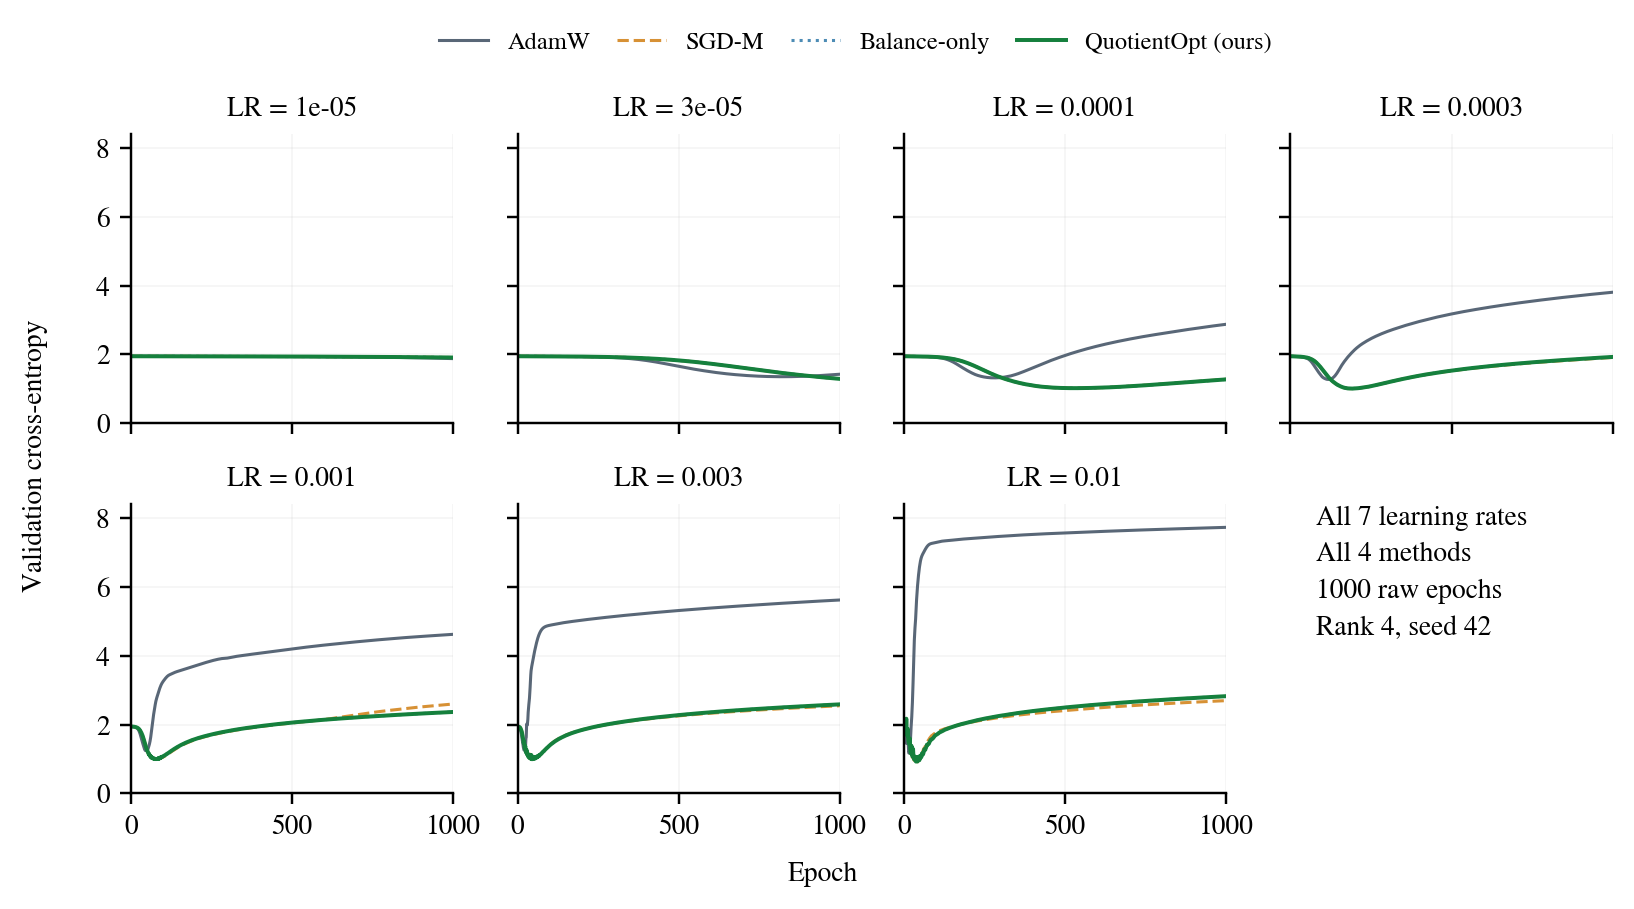
\includegraphics[width=.99\linewidth]{figures/cora_all_lr_loss.png}
\caption{Every learning rate in the complete Cora/GCN input-adapter
block: rank 4, seed 42, $\beta=0.9$. All four methods and all 1000
raw epoch observations are retained, with common axes, no smoothing,
and no omitted learning rates. This figure supplies the full learning-rate
context for the accuracy-selected core loss curves in
Figure~\ref{fig:core-loss}.}
\label{fig:all-lr-loss}
\end{figure}

\section{Stopped-Run Audit and Recovery Controls}
\label{app:failure-recovery}
\paragraph{Diagnostic stops versus objective failure.}
The original six stops comprise three diagnostic Gram-eigensolve exceptions, two JSON serialization exceptions, and one nonfinite training objective. A diagnostic exception is not evidence that the optimizer itself diverged. We replayed all six configurations with the same seed-42 CPU initialization, single-thread execution, float32 training, original learning rate, momentum, and 1000-update horizon. Only measurements and an unused pre-update diagnostic were changed. All available overlapping model checkpoints and training-loss observations are bit-identical, and the original stop records are retained.
The AdamW dense-$\kappa(Q)=10^4$ run now completes 1000 updates; its final loss is $0.80224$ and reconstruction error is $0.93624$. Thus AdamW completes all 12 prescribed gauges. After repairing logging, all five stopped SGD-M cases reach a genuinely nonfinite float32 training objective. The corrected fixed-step comparison has 43 complete runs and five objective failures; it does not attribute the AdamW diagnostic stop to optimization instability.
\paragraph{Measurement repair.}
For diagnostics only, let $B=U_B\Sigma_BV_B^\top$, $A=U_A\Sigma_AV_A^\top$, and $C=B^\top u_B-u_AA^\top$. The unregularized Sylvester measurement is evaluated in float64 by
\begin{equation}
\Omega=V_B\left[\frac{(V_B^\top C U_A)_{ij}}{s_i(B)^2+s_j(A)^2}\right]_{ij}U_A^\top,\qquad
(h_B,h_A)=(u_B-B\Omega,\ u_A+\Omega A).
\end{equation}
This avoids forming the diagnostic Gram spectra in float32. Reconstruction errors are also measured using float64 products and norms. Unavailable diagnostics are recorded as unavailable; they do not interrupt a finite optimizer update. Neither the AdamW/SGD-M update nor its gradients or optimizer state use this diagnostic projection.
\paragraph{A separate stabilization control.}
For each of the five genuinely failed SGD-M cases, we additionally run a disclosed recovery algorithm for all 1000 updates. This is a changed protocol, labeled SGD-M with Armijo backtracking and descent resets, following the sufficient-decrease principle of \citet{armijo1966minimization}. Its results never replace the fixed-step baseline. The original factors, observations, float32 gradient computation, and momentum coefficient $\beta=0.9$ are retained. Writing $z=(B,A)$, the candidate direction and acceptance rule are
\begin{align}
\widetilde v_t&=0.9v_{t-1}+g_t,\qquad g_t=\nabla F(z_t),\\
v_t&=\begin{cases}\widetilde v_t,&\langle g_t,\widetilde v_t\rangle>0,\\g_t,&\text{otherwise},\end{cases}\\
\eta_t^{(0)}&=\min\{10^{-3},2\eta_{t-1}\},\quad \eta_0=10^{-3},\quad \eta_t^{(k)}=2^{-k}\eta_t^{(0)},\\
F(z_t-\eta_t v_t)&\le F(z_t)-10^{-4}\eta_t\langle g_t,v_t\rangle
+10^{-7}\max\{1,|F(z_t)|\}.
\end{align}
The last term is the disclosed float32 acceptance tolerance. At most 60 trials are permitted per update. Every accepted step size, rejected trial count, reset, pre-update loss, post-update loss, and acceptance threshold is retained. All 5000 accepted updates satisfy the logged acceptance test and have finite losses. Completion indicates numerical stabilization under this changed protocol; the reconstruction errors below do not establish successful recovery of the planted matrix.
\begin{table}[ht]
\centering\small
\caption{All five SGD-M failure recoveries. The fixed-step column is the update at which the original $\eta=10^{-3}$ replay first encounters a nonfinite objective. The other columns describe the separate 1000-update backtracking protocol. Final loss is evaluated after the last update; $e_T=\|X_T-X_*\|_F/\|X_*\|_F$.}
\label{tab:failure-recovery}
\setlength{\tabcolsep}{3pt}
\begin{tabular}{llrrrrr}
\toprule Gauge & Value & Fixed-step failure & Final loss & Min.\ $\eta_t$ & Max.\ $\eta_t$ & $e_T$\\\midrule
scalar & $1.00\!\times\!10^{-3}$ & 5 & 0.8653 & $1.22\!\times\!10^{-7}$ & $3.91\!\times\!10^{-6}$ & 1.0059\\
scalar & $1.00\!\times\!10^{-2}$ & 8 & 0.8653 & $1.49\!\times\!10^{-11}$ & $2.50\!\times\!10^{-4}$ & 1.0059\\
scalar & $1.00\!\times\!10^{3}$ & 7 & 0.7944 & $7.81\!\times\!10^{-6}$ & $2.50\!\times\!10^{-4}$ & 0.9611\\
dense & $1.00\!\times\!10^{3}$ & 9 & 0.7873 & $1.91\!\times\!10^{-9}$ & $5.00\!\times\!10^{-4}$ & 0.9356\\
dense & $1.00\!\times\!10^{4}$ & 5 & 0.9679 & $3.64\!\times\!10^{-15}$ & $3.91\!\times\!10^{-6}$ & 0.9995\\
\bottomrule
\end{tabular}
\end{table}
The largest conditioning stresses require very small accepted steps, in some cases near numerical stagnation. These controls therefore separate three observations: diagnostic robustness, finite-step stability, and task recovery. They do not turn an unstable fixed-step baseline into a completed run of that same baseline.

\section{Fixed Expansion to Four Additional Tasks}
\label{app:new-task-expansion}
This exploratory expansion fixes four tasks before its formal runs:
CiteSeer/GCN \citep{kipf2017gcn} with a rank-4 input adapter; a synthetic sphere signed
distance field with a rank-8 SIREN \citep{sitzmann2020siren}; Burgers solution-operator learning
with a rank-8 DeepONet \citep{lu2019deeponet}; and $128\times128$ rank-8 matrix completion
with planted condition number 100. It is an additional task study,
not an independently confirmed or completed exhaustive proposal grid.
The SDF is synthetic. Burgers uses the documented Cole--Hopf
quadrature data and parameter-held-out splits from
Appendix~\ref{app:full-protocol}; it is not relabeled as a public
benchmark data set.

Each task crosses all four methods with exactly the same nine learning
rates
\[
\{10^{-5},3\!\times\!10^{-5},10^{-4},3\!\times\!10^{-4},
10^{-3},3\!\times\!10^{-3},10^{-2},3\!\times\!10^{-2},10^{-1}\}.
\]
We fix $\beta=0.9$, $\varepsilon=10^{-6}$, balance interval one,
and seed 42. The two larger step sizes extend the proposal's original
learning-rate slice equally for every method, to examine the
underfitting seen at its central setting. Graph runs have 1000 epochs;
the other runs have 2000. The four task blocks contain 36 attempts
each, for 144 total. Low-resource execution checks provide timing
estimates only and never enter the result tables.

\paragraph{Validation and test separation.}
Within a run, the earliest minimum-validation-loss checkpoint is
selected: cross-entropy for graphs and MSE for the other tasks.
Across learning rates, the minimum validation score selects a run,
with ties broken by smaller learning rate and then earlier epoch.
Test metrics never enter these choices. The additional implementation
does not evaluate the test set every epoch: it evaluates the
validation-selected checkpoint and final-horizon model after training.
The graph split is the official public transductive split; its metrics
are not presented as IID population-risk certificates.

Matrix completion uses disjoint fixed masks with 50\% training,
10\% validation, and 40\% test entries. Selection uses only the
validation-entry MSE. Full planted-matrix reconstruction error is
retained as a separate diagnostic and is not a validation criterion.
The other data and model definitions match the documented
implementation, including frozen base matrices and the shared
optimizer for non-factor parameters.

\paragraph{Complete blocks, stopped trials, and interpretation.}
A selected initial-slice comparison is published only after all 36
prescribed attempts for that task have terminated. The primary table selects from
completed full-horizon runs. If a later-stopped trial has a finite best
validation checkpoint, its test metric and status are retained in a
separate sensitivity analysis. A claim of improvement over all controls
must also survive that sensitivity analysis. Stopped runs are not
converted into complete-horizon results. Every attempted task,
learning rate, method, and failure remains in the full record below;
unfavorable outcomes are retained. One fixed seed does not establish
seed robustness or a confidence interval. Near-ties with balance-only
do not establish a distinct task-accuracy gain from projection.

\paragraph{Sequential factor-step extension.}
The initial 144-run plan remains unchanged and its complete comparisons
are retained separately in Table~\ref{tab:new-task-initial}.
Motivated by training underfitting and the different factor and
non-factor step scales, we add four factor learning rates
$\{0.3,1,3,10\}$ for every method and every task, fixing the shared
non-factor AdamW learning rate at $10^{-3}$.
Matrix completion has no non-factor parameters, so its four added
settings simply extend the factor learning-rate range.
This is a disclosed exploratory extension, not a setting fixed before
the initial study. It adds 64 trials. The joint budget has 13 settings
per method and 52 attempts per task, for 208 attempts in total.
All four methods receive the same two regimes: nine coupled learning
rates and four larger factor-only learning rates.
Joint selection minimizes validation loss over their union; a joint
comparison is reported only after all 52 attempts for that task have
terminated. The failed-trial sensitivity rule also applies to this
joint selection. Values below a validation MSE scale of $10^{-14}$
are treated as numerically limited when selecting substantive
case-study figures; percentage differences between such values do
not establish an optimization advantage.

\begin{table}[t]
\centering\small
\caption{Additional fixed four-family expansion. Each task has thirteen optimizer settings and four methods, with unchanged full horizons. Counts describe completed runs and recorded failures; a pending attempt is not a task result.}
\label{tab:new-task-status}
\begin{tabular}{lrrrr}
\toprule New task & Horizon & Planned & Complete & Failed\\\midrule
CiteSeer / GCN & 1000 & 52 & 52 & 0\\
SDF / SIREN & 2000 & 52 & 40 & 12\\
Burgers / DeepONet & 2000 & 52 & 45 & 7\\
Matrix completion & 2000 & 52 & 49 & 3\\
\bottomrule
\end{tabular}
\end{table}

\par\medskip\noindent\begin{minipage}{\linewidth}

\centering\small
\captionof{table}{Original nine-learning-rate expansion results before the separate factor-step extension. Every task has all 36 prescribed attempts terminated. Selection uses validation loss; the test loss is reported at its selected checkpoint. These initial outcomes, including unfavorable comparisons, are retained separately from the wider joint search.}
\label{tab:new-task-initial}
\begin{tabular}{lrrrr}
\toprule Task & AdamW & SGD-M & Balance & QO\\\midrule
CiteSeer / GCN & 1.2660 & \textbf{\boldmath 1.2125} & 1.2128 & \cellcolor{oursbg}1.2127\\
SDF / SIREN & $6.03\!\times\!10^{-5}$ & $2.42\!\times\!10^{-4}$ & $1.10\!\times\!10^{-5}$ & \cellcolor{oursgoodbg}\textbf{\boldmath $9.36\!\times\!10^{-6}$}\\
Burgers / DeepONet & \textbf{\boldmath $8.66\!\times\!10^{-5}$} & 0.0030 & 0.0035 & \cellcolor{oursbg}0.0042\\
Matrix completion & \textbf{\boldmath $1.06\!\times\!10^{-18}$} & $5.25\!\times\!10^{-8}$ & $3.90\!\times\!10^{-8}$ & \cellcolor{oursbg}$3.89\!\times\!10^{-8}$\\
\bottomrule
\end{tabular}

\end{minipage}\par\medskip

\par\medskip\noindent\begin{minipage}{\linewidth}

\centering\small
\captionof{table}{Validation-selected test losses in completed new-task blocks. All thirteen optimizer-setting attempts per method have finished before inclusion. Selection minimizes validation CE (graph) or validation MSE (other tasks), with ties by smaller LR then earlier epoch. Primary entries use full-horizon runs. Every trial, including failures and finite checkpoints from subsequently stopped trials, is retained in Appendix~\ref{app:new-task-expansion}. Lower is better.}
\label{tab:new-task-scores}
\begin{tabular}{lrrrr}
\toprule Task & AdamW & SGD-M & Balance & QO\\\midrule
CiteSeer / GCN & 1.3762 & 1.2508 & 1.2168 & \cellcolor{oursgoodbg}\textbf{\boldmath 1.2163}\\
SDF / SIREN & $6.03\!\times\!10^{-5}$ & $2.42\!\times\!10^{-4}$ & $1.10\!\times\!10^{-5}$ & \cellcolor{oursgoodbg}\textbf{\boldmath $9.36\!\times\!10^{-6}$}\\
Burgers / DeepONet & \textbf{\boldmath $8.66\!\times\!10^{-5}$} & 0.0030 & $5.85\!\times\!10^{-4}$ & \cellcolor{oursbg}0.0042\\
Matrix completion & \textbf{\boldmath $1.06\!\times\!10^{-18}$} & $1.17\!\times\!10^{-8}$ & $4.14\!\times\!10^{-17}$ & \cellcolor{oursbg}$4.65\!\times\!10^{-17}$\\
\bottomrule
\end{tabular}

\end{minipage}\par\medskip

\par\medskip\noindent\begin{minipage}{\linewidth}

\centering
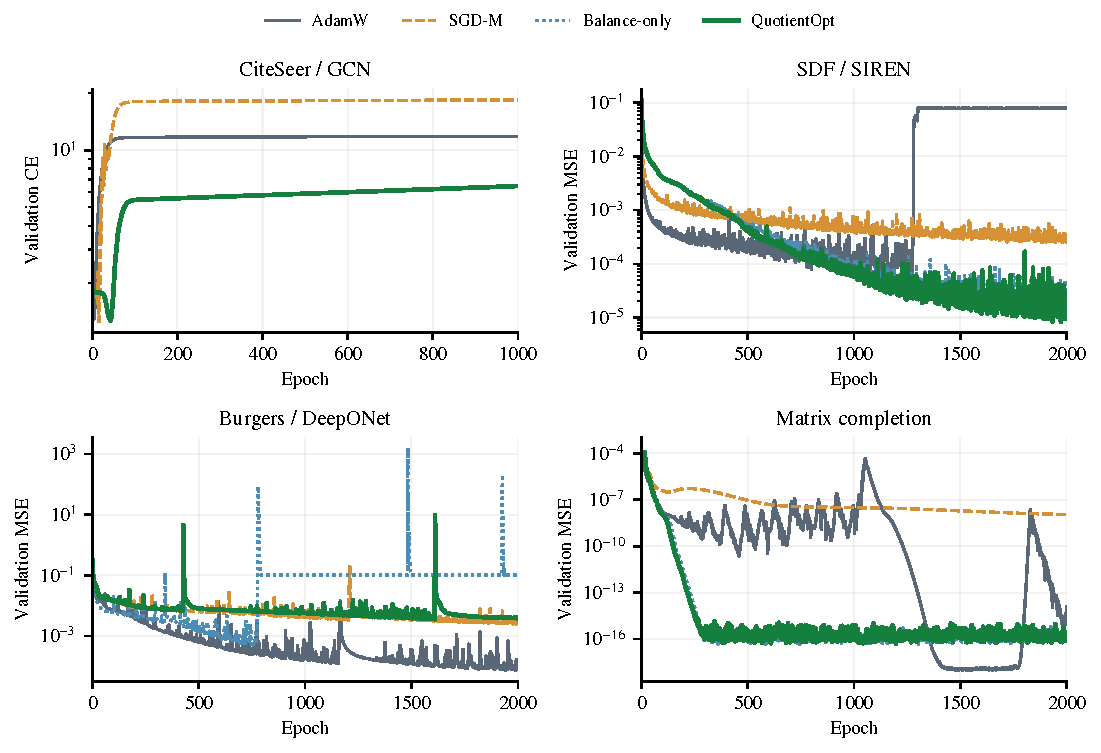
\includegraphics[width=.99\linewidth]{figures/new_task_complete_curves.pdf}
\captionof{figure}{All completed new-task comparison blocks, including unfavorable outcomes. For each method, validation loss selects the learning rate and checkpoint under the fixed rule; the entire selected run is plotted, with no smoothing or interval truncation. The curves are validation measurements, not IID risk certificates.}
\label{fig:new-task-curves}

\end{minipage}\par\medskip

\FloatBarrier
\paragraph{Descriptive validation iteration profiles.}
For regression tasks we additionally report the complete family of
relative-MSE targets $\{10^{-1},10^{-2},10^{-3},10^{-4},10^{-6}\}$.
With the same initial model and validation data for all methods,
define the finite-prefix tuning envelope
\begin{equation}
 e_{m,t}=\min_{\lambda\in\Lambda_m}
 \min_{0\le s\le\min\{t,T_{m,\lambda}\}}
 \frac{L_{\rm val}(z_{m,\lambda,s})}{L_{\rm val}(z_0)},
 \qquad
 \tau_m(a)=\inf\{t:e_{m,t}\le a\}.
\end{equation}
Every method has the same 13 optimizer settings. Retained finite
prefixes of stopped runs are eligible, so failed configurations do not
erase a baseline's earlier finite progress. An unreached target is
censored at the horizon. These are descriptive validation tuning
profiles, with test metrics excluded, rather than an independently
registered confirmation or a single executable optimizer trajectory.
They compare iteration budgets; shared-machine wall times are not a
controlled speed benchmark. The common initial validation scale is
checked against saved initial model states across methods and settings.
\par\medskip\noindent\begin{minipage}{\linewidth}

\centering\small
\captionof{table}{All descriptive validation-MSE targets in the new regression tasks. Each entry is the first epoch at which the validation tuning profile reaches the stated fraction of the common initial validation MSE. Every method has 13 optimizer settings; finite prefixes of later-stopped runs are eligible. A dash denotes an unreached target by epoch 2000. These are validation-selected iteration profiles, not wall-clock benchmarks or single executable training trajectories.}
\label{tab:new-task-hitting}
\begin{tabular}{lrrrrr}
\toprule Task & Relative target & AdamW & SGD-M & Balance & QO\\\midrule
SDF / SIREN & $10^{-1}$ & 2 & 2 & 2 & 2\\
SDF / SIREN & $10^{-2}$ & 11 & 28 & 16 & 17\\
SDF / SIREN & $10^{-3}$ & 157 & 1350 & 403 & 403\\
SDF / SIREN & $10^{-4}$ & \textemdash & \textemdash & 1183 & 1142\\
SDF / SIREN & $10^{-6}$ & \textemdash & \textemdash & \textemdash & \textemdash\\
Burgers / DeepONet & $10^{-1}$ & 73 & 292 & 47 & 47\\
Burgers / DeepONet & $10^{-2}$ & 297 & \textemdash & 651 & 584\\
Burgers / DeepONet & $10^{-3}$ & \textemdash & \textemdash & \textemdash & \textemdash\\
Burgers / DeepONet & $10^{-4}$ & \textemdash & \textemdash & \textemdash & \textemdash\\
Burgers / DeepONet & $10^{-6}$ & \textemdash & \textemdash & \textemdash & \textemdash\\
Matrix completion & $10^{-1}$ & 16 & 25 & 19 & 19\\
Matrix completion & $10^{-2}$ & 43 & 57 & 48 & 45\\
Matrix completion & $10^{-3}$ & 67 & 502 & 71 & 69\\
Matrix completion & $10^{-4}$ & 138 & \textemdash & 117 & 107\\
Matrix completion & $10^{-6}$ & 215 & \textemdash & 162 & 150\\
\bottomrule
\end{tabular}

\end{minipage}\par\medskip
\par\medskip\noindent\begin{minipage}{\linewidth}

\centering
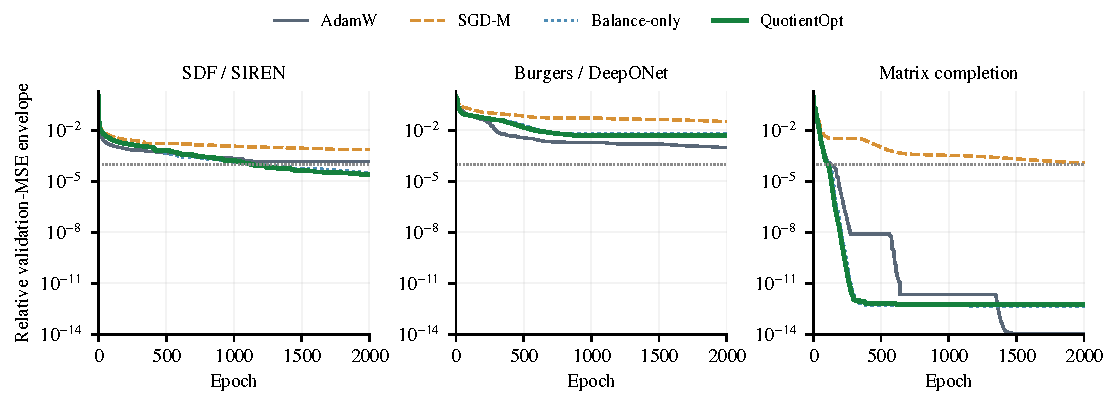
\includegraphics[width=.99\linewidth]{figures/new_task_convergence_profiles.pdf}
\captionof{figure}{Validation tuning envelopes from every completed regression-task block. At each epoch the envelope takes the best finite validation checkpoint among all 13 settings and earlier epochs, including prefixes of later-stopped trials. It is a descriptive equal-budget tuning profile, not one optimizer trajectory. The horizontal line is the $10^{-4}$ relative-MSE target; Table~\ref{tab:new-task-hitting} retains all five targets. Values below $10^{-14}$ are drawn at the plotting floor for legibility.}
\label{fig:new-task-convergence}

\end{minipage}\par\medskip

\FloatBarrier
\begingroup\small\setlength{\tabcolsep}{3pt}
\begin{longtable}{p{.34\linewidth}p{.09\linewidth}rrrr}
\caption{All attempted configurations in the new four-family expansion at this snapshot. Entries are validation-selected test losses, not test-minimized checkpoints; LR is the factor learning rate. Non-factor LR equals LR for the original nine settings through 0.1 and is fixed at $10^{-3}$ for the four added factor LRs 0.3, 1, 3, and 10. E is the selected epoch. C denotes a completed full-horizon run; F denotes a stopped run, whose best finite validation checkpoint is reported when available. Pending and running attempts have no final result and are omitted from this table. Their counts remain in Table~\ref{tab:new-task-status}.}\label{tab:new-task-all}\\
\toprule Task / method & LR & E & Val.\ score & Test loss & Status\\\midrule\endfirsthead
\toprule Task / method & LR & E & Val.\ score & Test loss & Status\\\midrule\endhead
CiteSeer / GCN / AdamW & 1e-05 & 1000 & 1.7272 & 1.7143 & C\\
CiteSeer / GCN / SGD-M & 1e-05 & 1000 & 1.7757 & 1.7693 & C\\
CiteSeer / GCN / Balance-only & 1e-05 & 1000 & 1.7757 & 1.7692 & C\\
\rowcolor{oursbg}CiteSeer / GCN / QuotientOpt & 1e-05 & 1000 & 1.7757 & 1.7692 & C\\
SDF / SIREN / AdamW & 1e-05 & 2000 & 0.0012 & 0.0015 & C\\
SDF / SIREN / SGD-M & 1e-05 & 2000 & 0.0049 & 0.0050 & C\\
SDF / SIREN / Balance-only & 1e-05 & 2000 & 0.0072 & 0.0063 & C\\
\rowcolor{oursbg}SDF / SIREN / QuotientOpt & 1e-05 & 2000 & 0.0072 & 0.0063 & C\\
Burgers / DeepONet / AdamW & 1e-05 & 2000 & 0.0014 & 0.0016 & C\\
Burgers / DeepONet / SGD-M & 1e-05 & 2000 & 0.0096 & 0.0113 & C\\
Burgers / DeepONet / Balance-only & 1e-05 & 2000 & 0.0096 & 0.0113 & C\\
\rowcolor{oursbg}Burgers / DeepONet / QuotientOpt & 1e-05 & 2000 & 0.0096 & 0.0113 & C\\
Matrix completion / AdamW & 1e-05 & 2000 & $7.56\!\times\!10^{-5}$ & $7.48\!\times\!10^{-5}$ & C\\
Matrix completion / SGD-M & 1e-05 & 725 & $9.10\!\times\!10^{-5}$ & $9.08\!\times\!10^{-5}$ & C\\
Matrix completion / Balance-only & 1e-05 & 2000 & $9.11\!\times\!10^{-5}$ & $9.11\!\times\!10^{-5}$ & C\\
\rowcolor{oursbg}Matrix completion / QuotientOpt & 1e-05 & 2000 & $9.11\!\times\!10^{-5}$ & $9.11\!\times\!10^{-5}$ & C\\
CiteSeer / GCN / AdamW & 3e-05 & 695 & 1.4035 & 1.3374 & C\\
CiteSeer / GCN / SGD-M & 3e-05 & 1000 & 1.3855 & 1.2792 & C\\
CiteSeer / GCN / Balance-only & 3e-05 & 1000 & 1.3852 & 1.2795 & C\\
\rowcolor{oursbg}CiteSeer / GCN / QuotientOpt & 3e-05 & 1000 & 1.3852 & 1.2795 & C\\
SDF / SIREN / AdamW & 3e-05 & 2000 & $3.56\!\times\!10^{-4}$ & $3.74\!\times\!10^{-4}$ & C\\
SDF / SIREN / SGD-M & 3e-05 & 1991 & 0.0020 & 0.0021 & C\\
SDF / SIREN / Balance-only & 3e-05 & 2000 & 0.0034 & 0.0031 & C\\
\rowcolor{oursbg}SDF / SIREN / QuotientOpt & 3e-05 & 2000 & 0.0033 & 0.0031 & C\\
Burgers / DeepONet / AdamW & 3e-05 & 2000 & $5.20\!\times\!10^{-4}$ & $5.85\!\times\!10^{-4}$ & C\\
Burgers / DeepONet / SGD-M & 3e-05 & 2000 & 0.0081 & 0.0095 & C\\
Burgers / DeepONet / Balance-only & 3e-05 & 2000 & 0.0082 & 0.0096 & C\\
\rowcolor{oursbg}Burgers / DeepONet / QuotientOpt & 3e-05 & 2000 & 0.0081 & 0.0096 & C\\
Matrix completion / AdamW & 3e-05 & 2000 & $2.08\!\times\!10^{-5}$ & $2.20\!\times\!10^{-5}$ & C\\
Matrix completion / SGD-M & 3e-05 & 247 & $9.10\!\times\!10^{-5}$ & $9.08\!\times\!10^{-5}$ & C\\
Matrix completion / Balance-only & 3e-05 & 2000 & $9.10\!\times\!10^{-5}$ & $9.10\!\times\!10^{-5}$ & C\\
\rowcolor{oursbg}Matrix completion / QuotientOpt & 3e-05 & 2000 & $9.10\!\times\!10^{-5}$ & $9.10\!\times\!10^{-5}$ & C\\
CiteSeer / GCN / AdamW & 0.0001 & 231 & 1.3392 & 1.2774 & C\\
CiteSeer / GCN / SGD-M & 0.0001 & 355 & 1.3561 & 1.2243 & C\\
CiteSeer / GCN / Balance-only & 0.0001 & 356 & 1.3555 & 1.2241 & C\\
\rowcolor{oursbg}CiteSeer / GCN / QuotientOpt & 0.0001 & 356 & 1.3560 & 1.2244 & C\\
SDF / SIREN / AdamW & 0.0001 & 1989 & $1.62\!\times\!10^{-4}$ & $1.64\!\times\!10^{-4}$ & C\\
SDF / SIREN / SGD-M & 0.0001 & 1998 & 0.0011 & 0.0011 & C\\
SDF / SIREN / Balance-only & 0.0001 & 2000 & $8.87\!\times\!10^{-4}$ & $8.74\!\times\!10^{-4}$ & C\\
\rowcolor{oursbg}SDF / SIREN / QuotientOpt & 0.0001 & 2000 & $6.94\!\times\!10^{-4}$ & $7.05\!\times\!10^{-4}$ & C\\
Burgers / DeepONet / AdamW & 0.0001 & 1990 & $1.34\!\times\!10^{-4}$ & $1.66\!\times\!10^{-4}$ & C\\
Burgers / DeepONet / SGD-M & 0.0001 & 1988 & 0.0063 & 0.0074 & C\\
Burgers / DeepONet / Balance-only & 0.0001 & 1995 & 0.0064 & 0.0076 & C\\
\rowcolor{oursbg}Burgers / DeepONet / QuotientOpt & 0.0001 & 1983 & 0.0064 & 0.0076 & C\\
Matrix completion / AdamW & 0.0001 & 2000 & $1.75\!\times\!10^{-6}$ & $1.77\!\times\!10^{-6}$ & C\\
Matrix completion / SGD-M & 0.0001 & 80 & $9.10\!\times\!10^{-5}$ & $9.08\!\times\!10^{-5}$ & C\\
Matrix completion / Balance-only & 0.0001 & 2000 & $9.08\!\times\!10^{-5}$ & $9.06\!\times\!10^{-5}$ & C\\
\rowcolor{oursbg}Matrix completion / QuotientOpt & 0.0001 & 2000 & $9.08\!\times\!10^{-5}$ & $9.06\!\times\!10^{-5}$ & C\\
CiteSeer / GCN / AdamW & 0.0003 & 96 & 1.3091 & 1.2485 & C\\
CiteSeer / GCN / SGD-M & 0.0003 & 139 & 1.3492 & 1.2123 & C\\
CiteSeer / GCN / Balance-only & 0.0003 & 139 & 1.3489 & 1.2128 & C\\
\rowcolor{oursbg}CiteSeer / GCN / QuotientOpt & 0.0003 & 138 & 1.3492 & 1.2152 & C\\
SDF / SIREN / AdamW & 0.0003 & 1994 & $1.22\!\times\!10^{-4}$ & $1.21\!\times\!10^{-4}$ & C\\
SDF / SIREN / SGD-M & 0.0003 & 1994 & $6.41\!\times\!10^{-4}$ & $6.72\!\times\!10^{-4}$ & C\\
SDF / SIREN / Balance-only & 0.0003 & 1997 & $6.74\!\times\!10^{-5}$ & $6.49\!\times\!10^{-5}$ & C\\
\rowcolor{oursbg}SDF / SIREN / QuotientOpt & 0.0003 & 1998 & $7.49\!\times\!10^{-5}$ & $8.96\!\times\!10^{-5}$ & C\\
Burgers / DeepONet / AdamW & 0.0003 & 1941 & $7.40\!\times\!10^{-5}$ & $8.66\!\times\!10^{-5}$ & C\\
Burgers / DeepONet / SGD-M & 0.0003 & 1977 & 0.0045 & 0.0053 & C\\
Burgers / DeepONet / Balance-only & 0.0003 & 1978 & 0.0047 & 0.0056 & C\\
\rowcolor{oursbg}Burgers / DeepONet / QuotientOpt & 0.0003 & 1997 & 0.0046 & 0.0055 & C\\
Matrix completion / AdamW & 0.0003 & 2000 & $3.14\!\times\!10^{-7}$ & $2.71\!\times\!10^{-7}$ & C\\
Matrix completion / SGD-M & 0.0003 & 2000 & $3.99\!\times\!10^{-5}$ & $3.87\!\times\!10^{-5}$ & C\\
Matrix completion / Balance-only & 0.0003 & 2000 & $9.02\!\times\!10^{-5}$ & $8.97\!\times\!10^{-5}$ & C\\
\rowcolor{oursbg}Matrix completion / QuotientOpt & 0.0003 & 2000 & $9.02\!\times\!10^{-5}$ & $8.97\!\times\!10^{-5}$ & C\\
CiteSeer / GCN / AdamW & 0.001 & 38 & 1.3143 & 1.2552 & C\\
CiteSeer / GCN / SGD-M & 0.001 & 53 & 1.3352 & 1.2125 & C\\
CiteSeer / GCN / Balance-only & 0.001 & 53 & 1.3358 & 1.2128 & C\\
\rowcolor{oursbg}CiteSeer / GCN / QuotientOpt & 0.001 & 53 & 1.3357 & 1.2127 & C\\
SDF / SIREN / AdamW & 0.001 & 1964 & $5.65\!\times\!10^{-5}$ & $8.43\!\times\!10^{-5}$ & C\\
SDF / SIREN / SGD-M & 0.001 & 1991 & $3.49\!\times\!10^{-4}$ & $3.97\!\times\!10^{-4}$ & C\\
SDF / SIREN / Balance-only & 0.001 & 1929 & $1.07\!\times\!10^{-5}$ & $1.10\!\times\!10^{-5}$ & C\\
\rowcolor{oursbg}SDF / SIREN / QuotientOpt & 0.001 & 1972 & $8.39\!\times\!10^{-6}$ & $9.36\!\times\!10^{-6}$ & C\\
Burgers / DeepONet / AdamW & 0.001 & 1957 & $1.45\!\times\!10^{-4}$ & $1.82\!\times\!10^{-4}$ & C\\
Burgers / DeepONet / SGD-M & 0.001 & 1977 & 0.0025 & 0.0030 & C\\
Burgers / DeepONet / Balance-only & 0.001 & 1944 & 0.0030 & 0.0036 & C\\
\rowcolor{oursbg}Burgers / DeepONet / QuotientOpt & 0.001 & 1608 & 0.0036 & 0.0042 & C\\
Matrix completion / AdamW & 0.001 & 2000 & $6.64\!\times\!10^{-8}$ & $7.12\!\times\!10^{-8}$ & C\\
Matrix completion / SGD-M & 0.001 & 2000 & $5.07\!\times\!10^{-6}$ & $4.95\!\times\!10^{-6}$ & C\\
Matrix completion / Balance-only & 0.001 & 2000 & $8.26\!\times\!10^{-5}$ & $8.12\!\times\!10^{-5}$ & C\\
\rowcolor{oursbg}Matrix completion / QuotientOpt & 0.001 & 2000 & $8.26\!\times\!10^{-5}$ & $8.12\!\times\!10^{-5}$ & C\\
CiteSeer / GCN / AdamW & 0.003 & 16 & 1.3068 & 1.2660 & C\\
CiteSeer / GCN / SGD-M & 0.003 & 28 & 1.3386 & 1.1922 & C\\
CiteSeer / GCN / Balance-only & 0.003 & 28 & 1.3401 & 1.1937 & C\\
\rowcolor{oursbg}CiteSeer / GCN / QuotientOpt & 0.003 & 28 & 1.3401 & 1.1937 & C\\
SDF / SIREN / AdamW & 0.003 & 1130 & $4.90\!\times\!10^{-5}$ & $6.03\!\times\!10^{-5}$ & C\\
SDF / SIREN / SGD-M & 0.003 & 1947 & $2.47\!\times\!10^{-4}$ & $2.42\!\times\!10^{-4}$ & C\\
SDF / SIREN / Balance-only & 0.003 & 1993 & $2.32\!\times\!10^{-5}$ & $2.63\!\times\!10^{-5}$ & C\\
\rowcolor{oursbg}SDF / SIREN / QuotientOpt & 0.003 & 1943 & $2.30\!\times\!10^{-5}$ & $2.40\!\times\!10^{-5}$ & C\\
Burgers / DeepONet / AdamW & 0.003 & 535 & $2.93\!\times\!10^{-4}$ & $3.50\!\times\!10^{-4}$ & C\\
Burgers / DeepONet / SGD-M & 0.003 & 585 & 0.0041 & 0.0049 & C\\
Burgers / DeepONet / Balance-only & 0.003 & 1978 & 0.0029 & 0.0035 & C\\
\rowcolor{oursbg}Burgers / DeepONet / QuotientOpt & 0.003 & 1519 & 0.0040 & 0.0047 & C\\
Matrix completion / AdamW & 0.003 & 1999 & $2.11\!\times\!10^{-8}$ & $2.20\!\times\!10^{-8}$ & C\\
Matrix completion / SGD-M & 0.003 & 2000 & $2.01\!\times\!10^{-6}$ & $1.84\!\times\!10^{-6}$ & C\\
Matrix completion / Balance-only & 0.003 & 2000 & $1.35\!\times\!10^{-5}$ & $1.26\!\times\!10^{-5}$ & C\\
\rowcolor{oursbg}Matrix completion / QuotientOpt & 0.003 & 2000 & $1.35\!\times\!10^{-5}$ & $1.26\!\times\!10^{-5}$ & C\\
CiteSeer / GCN / AdamW & 0.01 & 7 & 1.3692 & 1.3316 & C\\
CiteSeer / GCN / SGD-M & 0.01 & 19 & 1.3442 & 1.2166 & C\\
CiteSeer / GCN / Balance-only & 0.01 & 19 & 1.3505 & 1.2240 & C\\
\rowcolor{oursbg}CiteSeer / GCN / QuotientOpt & 0.01 & 19 & 1.3501 & 1.2234 & C\\
SDF / SIREN / AdamW & 0.01 & 39 & 0.0780 & 0.0747 & C\\
SDF / SIREN / SGD-M & 0.01 & 651 & $5.43\!\times\!10^{-4}$ & $5.49\!\times\!10^{-4}$ & C\\
SDF / SIREN / Balance-only & 0.01 & 412 & $2.46\!\times\!10^{-4}$ & $2.54\!\times\!10^{-4}$ & C\\
\rowcolor{oursbg}SDF / SIREN / QuotientOpt & 0.01 & 485 & $2.10\!\times\!10^{-4}$ & $2.13\!\times\!10^{-4}$ & C\\
Burgers / DeepONet / AdamW & 0.01 & 417 & 0.0040 & 0.0046 & C\\
Burgers / DeepONet / SGD-M & 0.01 & 41 & 0.1007 & 0.1177 & C\\
Burgers / DeepONet / Balance-only & 0.01 & 570 & 0.0069 & 0.0081 & C\\
\rowcolor{oursbg}Burgers / DeepONet / QuotientOpt & 0.01 & 770 & 0.0055 & 0.0065 & F\\
Matrix completion / AdamW & 0.01 & 2000 & $3.70\!\times\!10^{-10}$ & $3.87\!\times\!10^{-10}$ & C\\
Matrix completion / SGD-M & 0.01 & 2000 & $5.99\!\times\!10^{-7}$ & $5.46\!\times\!10^{-7}$ & C\\
Matrix completion / Balance-only & 0.01 & 2000 & $2.20\!\times\!10^{-6}$ & $2.15\!\times\!10^{-6}$ & C\\
\rowcolor{oursbg}Matrix completion / QuotientOpt & 0.01 & 2000 & $2.20\!\times\!10^{-6}$ & $2.15\!\times\!10^{-6}$ & C\\
CiteSeer / GCN / AdamW & 0.03 & 5 & 1.5255 & 1.5701 & C\\
CiteSeer / GCN / SGD-M & 0.03 & 27 & 1.3885 & 1.3170 & C\\
CiteSeer / GCN / Balance-only & 0.03 & 26 & 1.5585 & 1.4382 & C\\
\rowcolor{oursbg}CiteSeer / GCN / QuotientOpt & 0.03 & 26 & 1.5585 & 1.4382 & C\\
SDF / SIREN / AdamW & 0.03 & 9 & 0.0797 & 0.0746 & C\\
SDF / SIREN / SGD-M & 0.03 & 6 & 0.0786 & 0.0727 & F\\
SDF / SIREN / Balance-only & 0.03 & 147 & 0.0015 & 0.0016 & C\\
\rowcolor{oursbg}SDF / SIREN / QuotientOpt & 0.03 & 145 & 0.0020 & 0.0020 & C\\
Burgers / DeepONet / AdamW & 0.03 & 1278 & 0.0260 & 0.0242 & C\\
Burgers / DeepONet / SGD-M & 0.03 & 41 & 0.1007 & 0.1177 & C\\
Burgers / DeepONet / Balance-only & 0.03 & 62 & 0.1007 & 0.1177 & C\\
\rowcolor{oursbg}Burgers / DeepONet / QuotientOpt & 0.03 & 39 & 0.1007 & 0.1177 & F\\
Matrix completion / AdamW & 0.03 & 1540 & $9.61\!\times\!10^{-19}$ & $1.06\!\times\!10^{-18}$ & C\\
Matrix completion / SGD-M & 0.03 & 2000 & $2.06\!\times\!10^{-7}$ & $1.94\!\times\!10^{-7}$ & C\\
Matrix completion / Balance-only & 0.03 & 2000 & $3.64\!\times\!10^{-7}$ & $3.23\!\times\!10^{-7}$ & C\\
\rowcolor{oursbg}Matrix completion / QuotientOpt & 0.03 & 2000 & $3.63\!\times\!10^{-7}$ & $3.23\!\times\!10^{-7}$ & C\\
CiteSeer / GCN / AdamW & 0.1 & 22 & 1.6835 & 1.7497 & C\\
CiteSeer / GCN / SGD-M & 0.1 & 81 & 1.7301 & 1.7913 & C\\
CiteSeer / GCN / Balance-only & 0.1 & 100 & 1.7300 & 1.8034 & C\\
\rowcolor{oursbg}CiteSeer / GCN / QuotientOpt & 0.1 & 113 & 1.7375 & 1.8088 & C\\
SDF / SIREN / AdamW & 0.1 & 5 & 0.0900 & 0.0853 & C\\
SDF / SIREN / SGD-M & 0.1 & 1 & 0.3478 & 0.3722 & F\\
SDF / SIREN / Balance-only & 0.1 & 11 & 0.0791 & 0.0742 & F\\
\rowcolor{oursbg}SDF / SIREN / QuotientOpt & 0.1 & 13 & 0.0797 & 0.0755 & F\\
Burgers / DeepONet / AdamW & 0.1 & 1726 & 0.1006 & 0.1176 & C\\
Burgers / DeepONet / SGD-M & 0.1 & 170 & 0.0524 & 0.0578 & C\\
Burgers / DeepONet / Balance-only & 0.1 & 36 & 0.1007 & 0.1177 & C\\
\rowcolor{oursbg}Burgers / DeepONet / QuotientOpt & 0.1 & -- & \textemdash & \textemdash & F\\
Matrix completion / AdamW & 0.1 & 641 & $1.96\!\times\!10^{-16}$ & $1.88\!\times\!10^{-16}$ & C\\
Matrix completion / SGD-M & 0.1 & 2000 & $5.11\!\times\!10^{-8}$ & $5.25\!\times\!10^{-8}$ & C\\
Matrix completion / Balance-only & 0.1 & 2000 & $4.59\!\times\!10^{-8}$ & $3.90\!\times\!10^{-8}$ & C\\
\rowcolor{oursbg}Matrix completion / QuotientOpt & 0.1 & 2000 & $4.57\!\times\!10^{-8}$ & $3.89\!\times\!10^{-8}$ & C\\
CiteSeer / GCN / AdamW & 0.3 & 4 & 1.2942 & 1.3762 & C\\
CiteSeer / GCN / SGD-M & 0.3 & 33 & 1.3254 & 1.2699 & C\\
CiteSeer / GCN / Balance-only & 0.3 & 48 & 1.2749 & 1.1835 & C\\
\rowcolor{oursbg}CiteSeer / GCN / QuotientOpt & 0.3 & 48 & 1.2756 & 1.1842 & C\\
SDF / SIREN / AdamW & 0.3 & 182 & 0.0774 & 0.0726 & C\\
SDF / SIREN / SGD-M & 0.3 & 1 & 0.2931 & 0.3260 & F\\
SDF / SIREN / Balance-only & 0.3 & 1994 & $1.50\!\times\!10^{-4}$ & $1.70\!\times\!10^{-4}$ & C\\
\rowcolor{oursbg}SDF / SIREN / QuotientOpt & 0.3 & 1954 & $1.37\!\times\!10^{-4}$ & $1.54\!\times\!10^{-4}$ & C\\
Burgers / DeepONet / AdamW & 0.3 & 61 & 0.0317 & 0.0314 & C\\
Burgers / DeepONet / SGD-M & 0.3 & 22 & 0.1007 & 0.1177 & C\\
Burgers / DeepONet / Balance-only & 0.3 & 762 & $4.93\!\times\!10^{-4}$ & $5.85\!\times\!10^{-4}$ & C\\
\rowcolor{oursbg}Burgers / DeepONet / QuotientOpt & 0.3 & 910 & $3.62\!\times\!10^{-4}$ & $4.37\!\times\!10^{-4}$ & F\\
Matrix completion / AdamW & 0.3 & 2000 & $3.13\!\times\!10^{-9}$ & $2.98\!\times\!10^{-9}$ & C\\
Matrix completion / SGD-M & 0.3 & 2000 & $1.10\!\times\!10^{-8}$ & $1.17\!\times\!10^{-8}$ & C\\
Matrix completion / Balance-only & 0.3 & 2000 & $4.87\!\times\!10^{-9}$ & $4.25\!\times\!10^{-9}$ & C\\
\rowcolor{oursbg}Matrix completion / QuotientOpt & 0.3 & 2000 & $4.67\!\times\!10^{-9}$ & $4.08\!\times\!10^{-9}$ & C\\
CiteSeer / GCN / AdamW & 1 & 4 & 2.9122 & 2.9363 & C\\
CiteSeer / GCN / SGD-M & 1 & 26 & 1.3674 & 1.3193 & C\\
CiteSeer / GCN / Balance-only & 1 & 43 & 1.2690 & 1.2168 & C\\
\rowcolor{oursbg}CiteSeer / GCN / QuotientOpt & 1 & 43 & 1.2671 & 1.2163 & C\\
SDF / SIREN / AdamW & 1 & 67 & 0.0774 & 0.0727 & C\\
SDF / SIREN / SGD-M & 1 & -- & \textemdash & \textemdash & F\\
SDF / SIREN / Balance-only & 1 & 1980 & $1.36\!\times\!10^{-4}$ & $1.32\!\times\!10^{-4}$ & C\\
\rowcolor{oursbg}SDF / SIREN / QuotientOpt & 1 & 1995 & $1.40\!\times\!10^{-4}$ & $1.73\!\times\!10^{-4}$ & C\\
Burgers / DeepONet / AdamW & 1 & 36 & 0.1007 & 0.1177 & C\\
Burgers / DeepONet / SGD-M & 1 & 300 & 0.1007 & 0.1177 & C\\
Burgers / DeepONet / Balance-only & 1 & 29 & 0.1007 & 0.1177 & C\\
\rowcolor{oursbg}Burgers / DeepONet / QuotientOpt & 1 & 1 & 0.1332 & 0.1559 & F\\
Matrix completion / AdamW & 1 & 2000 & $5.79\!\times\!10^{-7}$ & $5.05\!\times\!10^{-7}$ & C\\
Matrix completion / SGD-M & 1 & 6 & $2.67\!\times\!10^{-5}$ & $2.70\!\times\!10^{-5}$ & F\\
Matrix completion / Balance-only & 1 & 2000 & $4.69\!\times\!10^{-7}$ & $1.98\!\times\!10^{-7}$ & C\\
\rowcolor{oursbg}Matrix completion / QuotientOpt & 1 & 2000 & $3.97\!\times\!10^{-7}$ & $1.87\!\times\!10^{-7}$ & C\\
CiteSeer / GCN / AdamW & 3 & 6 & 12.0411 & 14.8568 & C\\
CiteSeer / GCN / SGD-M & 3 & 23 & 1.3106 & 1.4144 & C\\
CiteSeer / GCN / Balance-only & 3 & 32 & 1.3635 & 1.3001 & C\\
\rowcolor{oursbg}CiteSeer / GCN / QuotientOpt & 3 & 32 & 1.3628 & 1.2997 & C\\
SDF / SIREN / AdamW & 3 & 429 & 0.0775 & 0.0730 & C\\
SDF / SIREN / SGD-M & 3 & -- & \textemdash & \textemdash & F\\
SDF / SIREN / Balance-only & 3 & 1 & 0.3028 & 0.3246 & F\\
\rowcolor{oursbg}SDF / SIREN / QuotientOpt & 3 & 1 & 0.3035 & 0.3098 & F\\
Burgers / DeepONet / AdamW & 3 & 35 & 0.1007 & 0.1177 & C\\
Burgers / DeepONet / SGD-M & 3 & 549 & 0.1007 & 0.1177 & C\\
Burgers / DeepONet / Balance-only & 3 & 30 & 0.1007 & 0.1177 & C\\
\rowcolor{oursbg}Burgers / DeepONet / QuotientOpt & 3 & 1 & 77.1926 & 76.3920 & F\\
Matrix completion / AdamW & 3 & 2000 & $6.52\!\times\!10^{-6}$ & $6.32\!\times\!10^{-6}$ & C\\
Matrix completion / SGD-M & 3 & 2 & $1.41\!\times\!10^{-4}$ & $1.36\!\times\!10^{-4}$ & F\\
Matrix completion / Balance-only & 3 & 2000 & $1.69\!\times\!10^{-6}$ & $1.39\!\times\!10^{-6}$ & C\\
\rowcolor{oursbg}Matrix completion / QuotientOpt & 3 & 2000 & $1.21\!\times\!10^{-6}$ & $1.04\!\times\!10^{-6}$ & C\\
CiteSeer / GCN / AdamW & 10 & 7 & 147.0064 & 185.7595 & C\\
CiteSeer / GCN / SGD-M & 10 & 16 & 1.2514 & 1.2508 & C\\
CiteSeer / GCN / Balance-only & 10 & 24 & 1.3988 & 1.3532 & C\\
\rowcolor{oursbg}CiteSeer / GCN / QuotientOpt & 10 & 24 & 1.3975 & 1.3524 & C\\
SDF / SIREN / AdamW & 10 & 1249 & 0.0774 & 0.0730 & C\\
SDF / SIREN / SGD-M & 10 & -- & \textemdash & \textemdash & F\\
SDF / SIREN / Balance-only & 10 & -- & \textemdash & \textemdash & F\\
\rowcolor{oursbg}SDF / SIREN / QuotientOpt & 10 & -- & \textemdash & \textemdash & F\\
Burgers / DeepONet / AdamW & 10 & 1583 & 0.1005 & 0.1175 & C\\
Burgers / DeepONet / SGD-M & 10 & 40 & 0.1007 & 0.1177 & C\\
Burgers / DeepONet / Balance-only & 10 & 37 & 0.1007 & 0.1177 & C\\
\rowcolor{oursbg}Burgers / DeepONet / QuotientOpt & 10 & 1 & 16.4258 & 16.4429 & F\\
Matrix completion / AdamW & 10 & 1941 & $9.48\!\times\!10^{-5}$ & $9.59\!\times\!10^{-5}$ & C\\
Matrix completion / SGD-M & 10 & 1 & 0.0011 & 0.0011 & F\\
Matrix completion / Balance-only & 10 & 1133 & $4.10\!\times\!10^{-17}$ & $4.14\!\times\!10^{-17}$ & C\\
\rowcolor{oursbg}Matrix completion / QuotientOpt & 10 & 1197 & $5.03\!\times\!10^{-17}$ & $4.65\!\times\!10^{-17}$ & C\\
\bottomrule
\end{longtable}
\endgroup
\paragraph{Stopped-checkpoint sensitivity: Burgers / DeepONet / QuotientOpt.} The minimum-validation-score checkpoint when stopped trials are eligible occurs at learning rate $0.3$ and epoch 910, with test loss $4.37\!\times\!10^{-4}$. The run status is failed. Its score is retained as a sensitivity control; it is not presented as a completed full-horizon run.

\FloatBarrier

\section{Adjusted Fixed-Step Recovery Study}
\label{app:failure-retry}
The original 208-attempt four-task search contains 22 numerical stops.
For each stopped configuration, the follow-up retains the same task,
model, rank, data, initialization, momentum coefficient, damping,
balance interval, non-factor learning rate, and 2000-epoch horizon.
The factor learning rate is lowered using completed runs in the same
task/method regime, with a separate protocol and run identifier.
The parent failure record and its finite validation checkpoint remain
in the original search. Every adjusted run begins from the identical
parent initial model, verified against its saved epoch-zero checkpoint.

The preflight evaluates three training epochs for each of nine distinct
task/method/step-scale groups. All 22 formal trajectories subsequently
contain exactly 2000 recorded epochs. The model within each run and the
reported retry configuration within a task/method group are chosen by
minimum validation MSE. Test measurements do not enter either choice.
No test measurements are present in the per-epoch trajectories.
Table~\ref{tab:retry-all} records every adjusted learning rate and
validation-selected outcome. The separate five genuinely failed
rank-one sensing SGD-M configurations have complete 1000-step Armijo
recovery controls in Appendix~\ref{app:failure-recovery}.
\begingroup\small\setlength{\tabcolsep}{4pt}
\begin{longtable}{@{}lrrrrr@{}}
\caption{All 22 adjusted fixed-step runs. Every row completes 2000 epochs. The parent learning rate produced a recorded numerical stop, and the adjusted learning rate uses the original initialization. Validation MSE determines the checkpoint; test MSE is measured at that selected checkpoint.}\label{tab:retry-all}\\
\toprule Task / method & Parent LR & Retry LR & Epoch & Val. MSE & Test MSE\\\midrule\endfirsthead
\toprule Task / method & Parent LR & Retry LR & Epoch & Val. MSE & Test MSE\\\midrule\endhead
\rowcolor{oursbg}Burgers / DeepONet / QuotientOpt & 0.01 & 0.00255 & 1780 & 0.0021 & 0.0025\\
\rowcolor{oursbg}Burgers / DeepONet / QuotientOpt & 0.03 & 0.0021 & 1792 & 0.0031 & 0.0037\\
\rowcolor{oursbg}Burgers / DeepONet / QuotientOpt & 0.1 & 0.00165 & 1695 & 0.0031 & 0.0036\\
\rowcolor{oursbg}Burgers / DeepONet / QuotientOpt & 0.3 & 0.00255 & 1992 & 0.0029 & 0.0034\\
\rowcolor{oursbg}Burgers / DeepONet / QuotientOpt & 1 & 0.00225 & 1995 & 0.0029 & 0.0035\\
\rowcolor{oursbg}Burgers / DeepONet / QuotientOpt & 3 & 0.00195 & 1993 & 0.0028 & 0.0033\\
\rowcolor{oursbg}Burgers / DeepONet / QuotientOpt & 10 & 0.00165 & 1995 & 0.0031 & 0.0037\\
SDF / SIREN / SGD-M & 0.03 & 0.0085 & 1785 & $1.12\!\times\!10^{-4}$ & $1.09\!\times\!10^{-4}$\\
SDF / SIREN / SGD-M & 0.1 & 0.0055 & 1934 & $1.68\!\times\!10^{-4}$ & $1.85\!\times\!10^{-4}$\\
SDF / SIREN / SGD-M & 0.3 & 0.0085 & 1981 & $2.17\!\times\!10^{-4}$ & $2.52\!\times\!10^{-4}$\\
SDF / SIREN / SGD-M & 1 & 0.0075 & 1997 & $2.26\!\times\!10^{-4}$ & $2.49\!\times\!10^{-4}$\\
SDF / SIREN / SGD-M & 3 & 0.0065 & 1977 & $2.53\!\times\!10^{-4}$ & $2.81\!\times\!10^{-4}$\\
SDF / SIREN / SGD-M & 10 & 0.0055 & 1994 & $2.73\!\times\!10^{-4}$ & $3.00\!\times\!10^{-4}$\\
SDF / SIREN / Balance-only & 0.1 & 0.0255 & 146 & 0.0018 & 0.0018\\
SDF / SIREN / Balance-only & 3 & 0.85 & 1974 & $1.20\!\times\!10^{-4}$ & $1.35\!\times\!10^{-4}$\\
SDF / SIREN / Balance-only & 10 & 0.55 & 1998 & $1.36\!\times\!10^{-4}$ & $1.45\!\times\!10^{-4}$\\
\rowcolor{oursbg}SDF / SIREN / QuotientOpt & 0.1 & 0.0255 & 163 & 0.0014 & 0.0015\\
\rowcolor{oursbg}SDF / SIREN / QuotientOpt & 3 & 0.85 & 1984 & $1.41\!\times\!10^{-4}$ & $1.40\!\times\!10^{-4}$\\
\rowcolor{oursbg}SDF / SIREN / QuotientOpt & 10 & 0.55 & 1957 & $1.29\!\times\!10^{-4}$ & $1.40\!\times\!10^{-4}$\\
Matrix completion / SGD-M & 1 & 0.255 & 2000 & $2.24\!\times\!10^{-8}$ & $2.48\!\times\!10^{-8}$\\
Matrix completion / SGD-M & 3 & 0.21 & 2000 & $3.77\!\times\!10^{-8}$ & $4.06\!\times\!10^{-8}$\\
Matrix completion / SGD-M & 10 & 0.165 & 2000 & $3.69\!\times\!10^{-8}$ & $4.08\!\times\!10^{-8}$\\
\bottomrule
\end{longtable}
\endgroup


\section{Conditional Initialization Confirmations}
\label{app:initialization-confirmation}
We additionally freeze the validation-selected learning rates from
the original Cora seven-learning-rate loss-based analysis
(Table~\ref{tab:secondary-ce}) and the complete SDF nine-learning-rate
analysis (Table~\ref{tab:new-task-initial}). Each method then runs
three model initializations, 42, 43, and 44, without learning-rate
retuning across initializations. Cora uses 1000 epochs and SDF uses
2000. This adds 24 full-horizon attempts across all four methods.

Data generation, split masks, and shuffle RNG remain at seed 42.
Only the model initialization changes. A paired initialization has
identical initial model states across the four methods; the three
initializations have distinct model states. A protocol audit checks
these properties against saved initial checkpoints, data tensors,
split indices, and RNG states. Initialization 42 is rerun on CPU so
all three confirmation runs use the same execution setting.
This audit fixes data, initial models, and RNG states; it does not
assert bitwise-identical floating-point optimization trajectories.

Within each run the earliest minimum-validation-loss checkpoint is
selected, with test metrics excluded. Every individual result and
failure is retained. Mean and sample SD are reported only when all
three full-horizon runs for that method complete. The SD describes
conditional initialization variability on one fixed data split;
these checks do not constitute independent-data replications or
a population-risk confidence interval.

\par\medskip\noindent\begin{minipage}{\linewidth}

\centering\small
\captionof{table}{Conditional initialization confirmation. Data and shuffle seed stay fixed at 42; only model initialization changes over 42, 43, 44. Each method uses its frozen parent-selected learning rate, with no retuning across initializations. Test loss is measured at the validation-selected checkpoint. Mean $\pm$ sample SD is shown only for three completed runs. This SD does not describe independent-data uncertainty.}
\label{tab:initialization-confirmation}
\begin{tabular}{llrrr}
\toprule Task & Method & LR & Complete/3 & Test loss mean $\pm$ SD\\\midrule
Cora / GCN & AdamW & 0.01 & 3/3 & $1.1376\pm0.0793$\\
Cora / GCN & SGD-M & 0.01 & 3/3 & $0.8741\pm0.0562$\\
Cora / GCN & Balance-only & 0.01 & 3/3 & $0.8807\pm0.0551$\\
\rowcolor{oursbg}Cora / GCN & QuotientOpt & 0.01 & 3/3 & $0.8807\pm0.0552$\\
SDF / SIREN & AdamW & 0.003 & 3/3 & $(6.21\pm0.17)\!\times\!10^{-5}$\\
SDF / SIREN & SGD-M & 0.003 & 3/3 & $(2.62\pm0.62)\!\times\!10^{-4}$\\
SDF / SIREN & Balance-only & 0.001 & 3/3 & $(1.18\pm0.07)\!\times\!10^{-5}$\\
\rowcolor{oursbg}SDF / SIREN & QuotientOpt & 0.001 & 3/3 & $(1.10\pm0.26)\!\times\!10^{-5}$\\
\bottomrule
\end{tabular}

\end{minipage}\par\medskip
\FloatBarrier
\begingroup\small\setlength{\tabcolsep}{3pt}
\begin{longtable}{p{.31\linewidth}rrrrrr}
\caption{Every initialization outcome. F is a stopped run; its finite validation-selected checkpoint is retained when available. No initialization is dropped from the record.}\label{tab:initialization-all}\\
\toprule Task / method & Init. & LR & Epoch & Val.\ loss & Test loss & Status\\\midrule\endfirsthead
\toprule Task / method & Init. & LR & Epoch & Val.\ loss & Test loss & Status\\\midrule\endhead
Cora / GCN / AdamW & 42 & 0.01 & 15 & 1.1728 & 1.0525 & C\\
Cora / GCN / SGD-M & 42 & 0.01 & 36 & 0.9079 & 0.8579 & C\\
Cora / GCN / Balance-only & 42 & 0.01 & 37 & 0.9141 & 0.8646 & C\\
\rowcolor{oursbg}Cora / GCN / QuotientOpt & 42 & 0.01 & 37 & 0.9141 & 0.8646 & C\\
Cora / GCN / AdamW & 43 & 0.01 & 12 & 1.2179 & 1.1510 & C\\
Cora / GCN / SGD-M & 43 & 0.01 & 35 & 0.8879 & 0.8278 & C\\
Cora / GCN / Balance-only & 43 & 0.01 & 35 & 0.8807 & 0.8355 & C\\
\rowcolor{oursbg}Cora / GCN / QuotientOpt & 43 & 0.01 & 35 & 0.8806 & 0.8355 & C\\
Cora / GCN / AdamW & 44 & 0.01 & 13 & 1.3324 & 1.2093 & C\\
Cora / GCN / SGD-M & 44 & 0.01 & 29 & 1.0943 & 0.9367 & C\\
Cora / GCN / Balance-only & 44 & 0.01 & 29 & 1.0953 & 0.9420 & C\\
\rowcolor{oursbg}Cora / GCN / QuotientOpt & 44 & 0.01 & 29 & 1.0955 & 0.9422 & C\\
SDF / SIREN / AdamW & 42 & 0.003 & 1130 & $4.90\!\times\!10^{-5}$ & $6.03\!\times\!10^{-5}$ & C\\
SDF / SIREN / SGD-M & 42 & 0.003 & 1947 & $2.47\!\times\!10^{-4}$ & $2.42\!\times\!10^{-4}$ & C\\
SDF / SIREN / Balance-only & 42 & 0.001 & 1956 & $1.02\!\times\!10^{-5}$ & $1.18\!\times\!10^{-5}$ & C\\
\rowcolor{oursbg}SDF / SIREN / QuotientOpt & 42 & 0.001 & 1993 & $1.25\!\times\!10^{-5}$ & $1.39\!\times\!10^{-5}$ & C\\
SDF / SIREN / AdamW & 43 & 0.003 & 978 & $5.77\!\times\!10^{-5}$ & $6.37\!\times\!10^{-5}$ & C\\
SDF / SIREN / SGD-M & 43 & 0.003 & 1994 & $2.99\!\times\!10^{-4}$ & $3.32\!\times\!10^{-4}$ & C\\
SDF / SIREN / Balance-only & 43 & 0.001 & 1997 & $1.09\!\times\!10^{-5}$ & $1.10\!\times\!10^{-5}$ & C\\
\rowcolor{oursbg}SDF / SIREN / QuotientOpt & 43 & 0.001 & 1975 & $8.90\!\times\!10^{-6}$ & $8.84\!\times\!10^{-6}$ & C\\
SDF / SIREN / AdamW & 44 & 0.003 & 1111 & $5.94\!\times\!10^{-5}$ & $6.25\!\times\!10^{-5}$ & C\\
SDF / SIREN / SGD-M & 44 & 0.003 & 1980 & $1.88\!\times\!10^{-4}$ & $2.12\!\times\!10^{-4}$ & C\\
SDF / SIREN / Balance-only & 44 & 0.001 & 1968 & $1.19\!\times\!10^{-5}$ & $1.25\!\times\!10^{-5}$ & C\\
\rowcolor{oursbg}SDF / SIREN / QuotientOpt & 44 & 0.001 & 1993 & $1.05\!\times\!10^{-5}$ & $1.04\!\times\!10^{-5}$ & C\\
\bottomrule
\end{longtable}
\endgroup


\paragraph{Matrix-completion target confirmation.}
An additional 12 runs use initializations 42, 43, and 44 with the
same planted matrix and disjoint masks. Each method's step size is
frozen from its earliest parent validation hit at the relative-MSE
target $10^{-4}$; SGD-M, which never reaches it in the parent search,
uses its minimum-validation-loss completed configuration.
The initial model changes while data generation and mask RNG remain
fixed. The common initial validation MSE is recorded separately for
each paired initialization. No step size is retuned across these
checks. Every failure and unreached target is retained; initialization
means are reported only for three observed target hits.
\par\medskip\noindent\begin{minipage}{\linewidth}

\centering\small
\captionof{table}{Matrix-completion initialization confirmation with frozen step sizes selected by the parent validation target. Data and masks stay fixed; model initializations are 42, 43, 44. The target is $10^{-4}$ of the common initial validation MSE of each paired initialization. Every initialization is retained; an unreached target is censored at 2000 epochs. Mean $\pm$ initialization SD is shown only if all three runs reach the target.}
\label{tab:matrix-initialization}
\begin{tabular}{lrrrr}
\toprule Method & LR & Complete/3 & Reached/3 & Epochs mean $\pm$ SD\\\midrule
AdamW & 0.03 & 3/3 & 3/3 & $118.7\pm16.9$\\
SGD-M & 0.3 & 3/3 & 2/3 & \textemdash\\
Balance-only & 10 & 3/3 & 2/3 & \textemdash\\
\rowcolor{oursbg}QuotientOpt & 10 & 3/3 & 2/3 & \textemdash\\
\bottomrule
\end{tabular}

\end{minipage}\par\medskip
\par\medskip\noindent\begin{minipage}{\linewidth}

\centering\small
\captionof{table}{Every matrix-completion initialization: first epoch reaching the target. A dash denotes an unreached target, not an omitted trial. All full-horizon and failure records are retained.}
\label{tab:matrix-initialization-all}
\begin{tabular}{rrrrr}
\toprule Init. & AdamW & SGD-M & Balance & QO\\\midrule
42 & 138 & \textemdash & 117 & 107\\
43 & 107 & 1234 & \textemdash & \textemdash\\
44 & 111 & 1851 & 105 & 171\\
\bottomrule
\end{tabular}

\end{minipage}\par\medskip

\FloatBarrier

\section{Additional Complete Loss Trajectories}
\label{app:supporting-loss}
\begin{figure}[t]
\centering
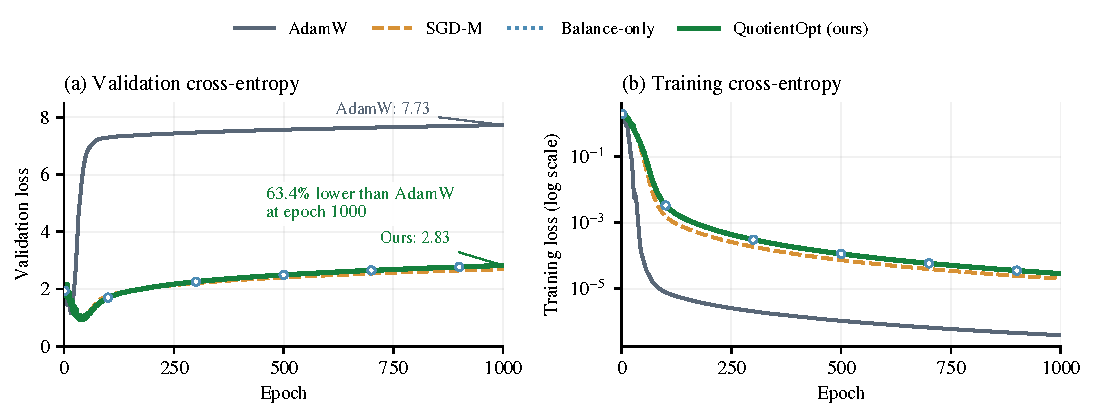
\includegraphics[width=.99\linewidth]{figures/core_loss_cora.pdf}
\caption{\textbf{Core loss curves: lower validation loss than AdamW.}
Cora/GCN input adapter, rank 4, seed 42, $\beta=0.9$.
The complete seven-learning-rate block selects $\eta=10^{-2}$ for
every method using validation accuracy; test metrics do not enter
selection. All 1000 raw epoch observations are shown without smoothing
or interval truncation. (a) Validation cross-entropy: QuotientOpt's
final loss is $63.4\%$ below AdamW's, while SGD-M is slightly lower
and balance-only nearly overlaps QuotientOpt. Open green circles
identify the overlapping balance-only trajectory.
(b) Training cross-entropy on a logarithmic scale: AdamW attains
the smallest training loss.}
\label{fig:core-loss}
\end{figure}
\begin{figure}[t]
\centering
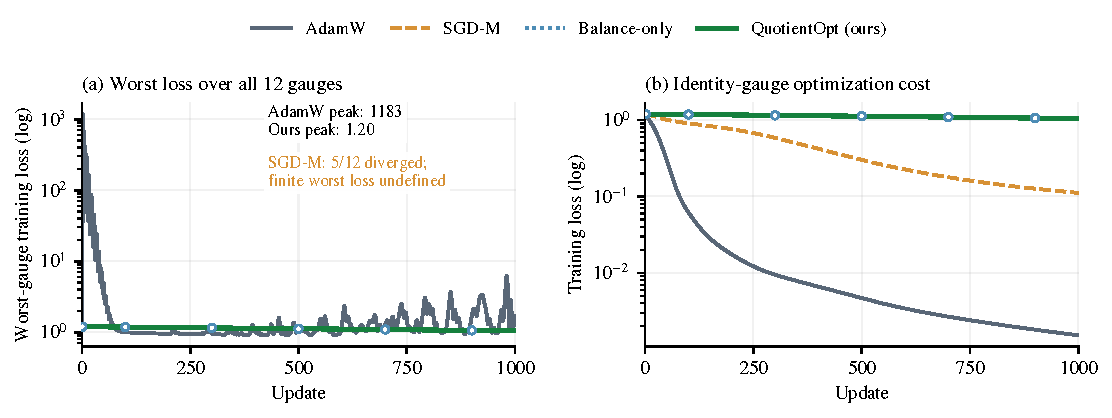
\includegraphics[width=.99\linewidth]{figures/core_loss_gauge.pdf}
\caption{\textbf{Core sensing loss curves: robustness and optimization cost.}
True rank-one sensing, $128\times128$, rank 16, 19,200 observations,
seed 42, $\eta=10^{-3}$, $\beta=0.9$; all 1000 raw observations
and logarithmic loss axes. (a) At each update, the maximum training
loss over every one of the 12 prescribed gauges. AdamW and both
balanced arms have all 12 completed trajectories. The five confirmed
SGD-M failures preclude a finite 12-gauge envelope; an envelope of
only its successful cases is not substituted.
(b) The identity-gauge reference: AdamW fits this problem much better
at the fixed learning rate. Both panels retain the overlapping
balance-only control. The gain in (a) is gauge robustness, not faster
identity-gauge recovery or an accuracy gain uniquely due to projection.}
\label{fig:core-gauge-loss}
\end{figure}
\begin{figure}[t]
\centering
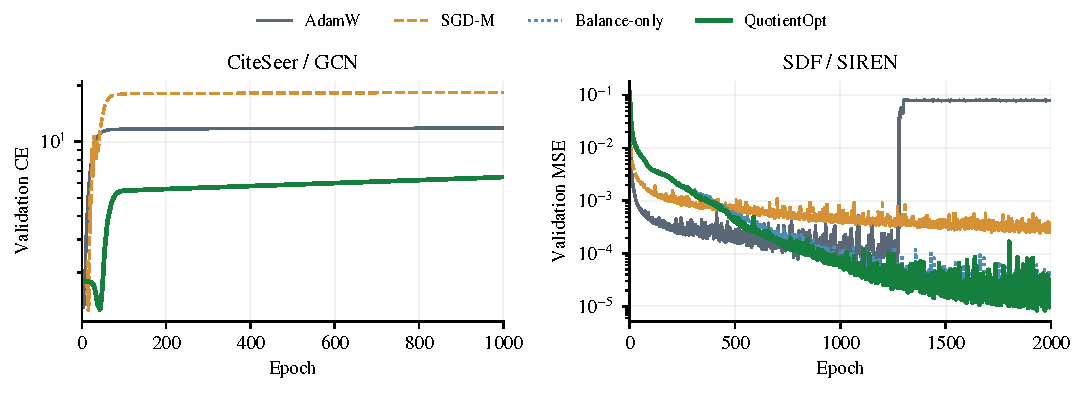
\includegraphics[width=.99\linewidth]{figures/new_task_validation_cases.pdf}
\caption{Exploratory validation-loss case studies from completed new-task blocks. The presentation rule requires at least 1\% lower minimum validation loss for a full-horizon QuotientOpt run than AdamW, including its best finite stopped-trial checkpoints; test outcomes do not select panels. Every method receives the same thirteen-setting optimizer budget and every selected trajectory is shown in full. All four methods are retained. This selected-case figure does not establish improvement over every baseline. All tasks, test metrics, and unfavorable outcomes are retained in Table~\ref{tab:new-task-scores} and Appendix~\ref{app:new-task-expansion}.}
\label{fig:new-task-validation-cases}
\end{figure}
\begin{figure}[t]
\centering
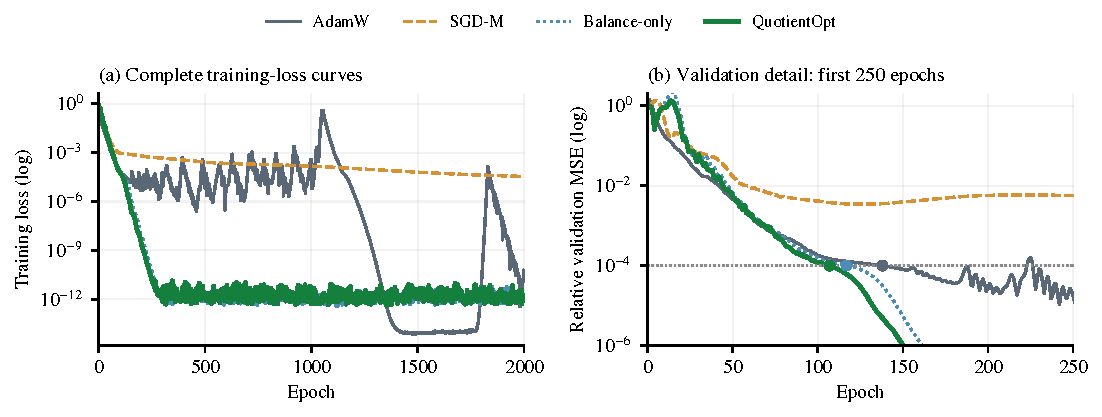
\includegraphics[width=.99\linewidth]{figures/new_matrix_convergence_raw.pdf}
\caption{\textbf{Additional matrix-completion loss curves.} Rank 8, planted condition 100, $128\times128$, seed 42. Each method selects its setting by the earliest validation epoch reaching $10^{-4}$ of the common initial validation MSE, over the same 13-setting budget. For SGD-M, which never reaches the target, the minimum-validation-loss full-horizon setting is shown. (a) Complete raw training-loss observations, without smoothing. (b) A common first-250-epoch validation zoom, with first-hitting points and the target line. These are actual selected-run trajectories. Figure~\ref{fig:new-task-convergence} separately reports tuning envelopes; the full record includes every setting and stopped prefix.}
\label{fig:new-matrix-raw}
\end{figure}
\begin{figure}[t]
\centering
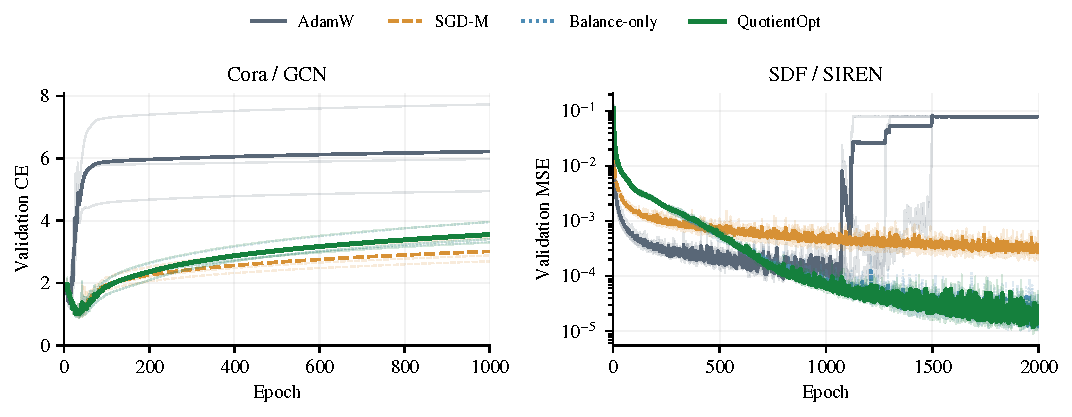
\includegraphics[width=.99\linewidth]{figures/initialization_confirmation_curves.pdf}
\caption{\textbf{Conditional initialization loss checks.} Data and shuffle seed 42 are fixed, with model initializations 42, 43, and 44. Parent-selected learning rates are frozen per method, with no per-initialization retuning. Thin lines show every initialization; thick lines show their arithmetic mean validation loss at each epoch. All raw epochs are retained without smoothing. The mean curves are descriptive summaries, not confidence bands. Test outcomes and all four controls are retained in Table~\ref{tab:initialization-confirmation}.}
\label{fig:initialization-loss}
\end{figure}
\FloatBarrier

\section{Initial Central-Setting Comparisons}
\label{app:initial-central}
\par\medskip\noindent\begin{minipage}{\linewidth}

\centering
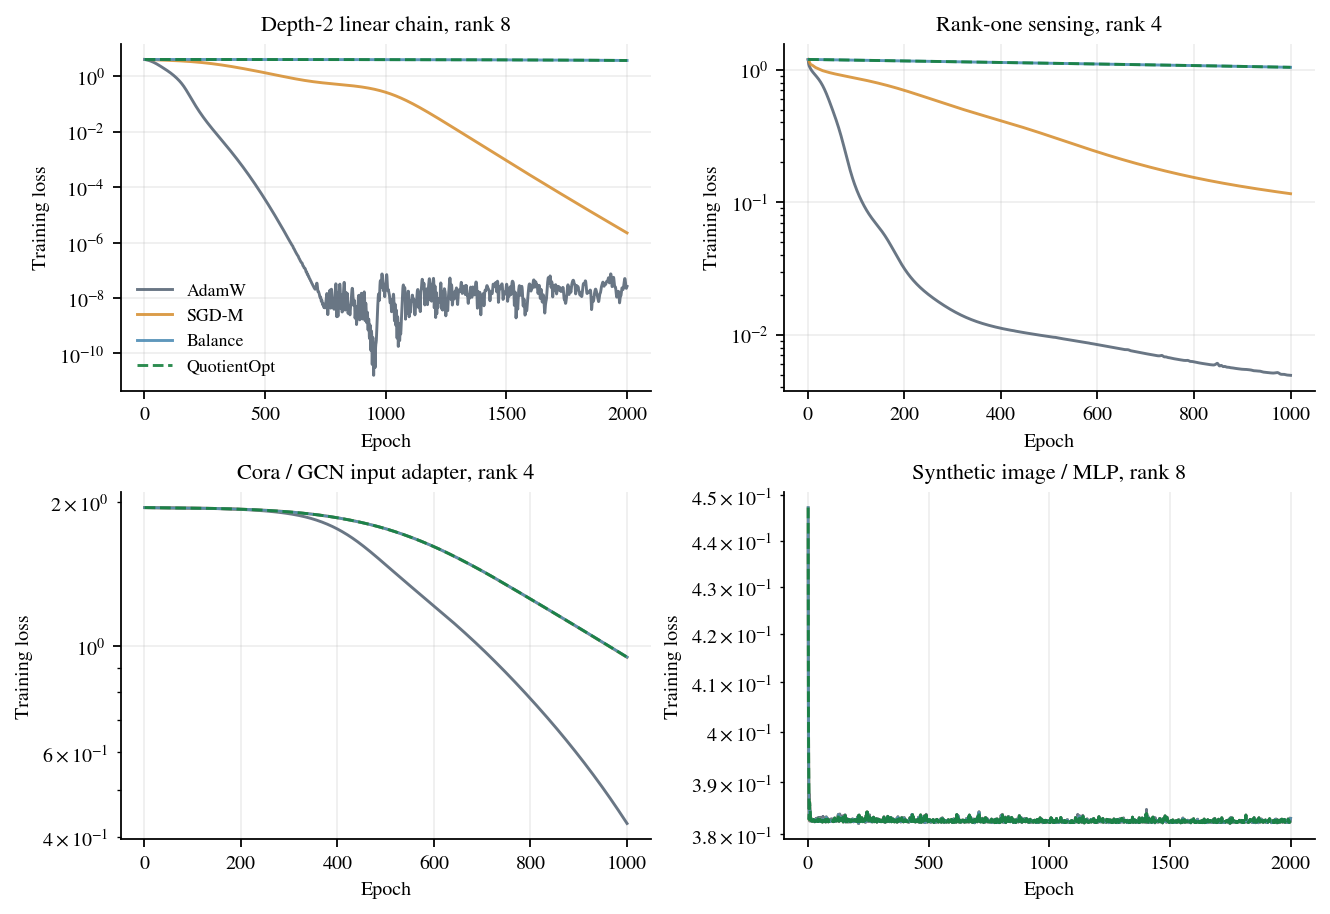
\includegraphics[width=.98\linewidth]{figures/replacement_trajectories.png}
\captionof{figure}{Initial completed central-setting replacement cohorts, before exhaustive tuning. The four panels show all four families with a matched completed cohort at the figure snapshot: 2000 epochs for depth-2 chains, sensing, and INR; 1000 epochs for Cora. The balanced momentum methods nearly overlap. AdamW optimizes the chain and sensing objectives much better at this setting; lower training loss on Cora does not imply higher test accuracy. These trajectories do not establish a best-tuned-method comparison.}
\label{fig:replacement-curves}

\end{minipage}\par\medskip

\paragraph{Central-setting outcomes across families.} At the displayed central setting, Cora/GCN's final test accuracy is $69.9\%$ for balance-only and QuotientOpt, versus $66.5\%$ for AdamW and $70.2\%$ for SGD-M. This is a positive comparison against AdamW, not against the stronger SGD-M endpoint. On the initial rank-one sensing and depth-2 chain cohorts, AdamW has substantially smaller final reconstruction error than the balanced momentum arms. The initial INR/MLP cohort has nearly tied held-out error across all four methods. Figure~\ref{fig:replacement-curves} reports the corresponding complete training trajectories. The search remains incomplete, so these are scoped central-setting outcomes, not conclusions from the full learning-rate/momentum/rank grid.

\FloatBarrier
\section{Completed Replacement Experiments}
\label{app:new-results}
Only complete runs with the configured horizon and a saved result record enter these tables. Runs from the two-epoch implementation checks are excluded. This snapshot is generated from the experiment artifacts and can grow as the full grid executes. A cohort requires all four methods at a matched task/rank/hyperparameter setting; partial cohorts remain in the progress record without a winner label.
\begin{longtable}{p{.31\linewidth}p{.13\linewidth}rrrr}
\caption{Completed matched main-experiment four-method cohorts. Gauge and ablation runs are reported separately. Values are final task metrics: planted-operator reconstruction error for matrix/chain tasks, held-out metrics for other tasks. Lower error is better; higher accuracy/PSNR is better. Only the first 30 cohorts are typeset here; all records remain in the machine-readable progress artifact.}\label{tab:new-results}\\
\toprule Task & Metric & AdamW & SGD-M & Balance & QO \\ \midrule\endfirsthead
\toprule Task & Metric & AdamW & SGD-M & Balance & QO \\ \midrule\endhead
\shortstack[l]{poisson/pinn\\r16, lr=0.001} & Rel. $L_2$ & 0.06223 & 0.07767 & 0.05577 & 0.05384\\
\shortstack[l]{synthetic/chain\\r8/L2, lr=0.001} & Rel. error & 0.06798 & 0.06799 & 0.9579 & 0.9579\\
\shortstack[l]{cora/gcn\\r4, lr=1e-05} & Accuracy & 0.452 & 0.4 & 0.401 & 0.401\\
\shortstack[l]{synthetic/chain\\r8/L2, lr=0.001} & Rel. error & 0.01359 & 0.01363 & 0.959 & 0.959\\
\shortstack[l]{cifar10/mlp\\r32, lr=0.001} & Accuracy & 0.4942 & 0.4782 & 0.4723 & 0.4724\\
\shortstack[l]{image/mlp\\r8, lr=0.001} & PSNR & 4.536 & 4.539 & 4.539 & 4.539\\
\shortstack[l]{sensing/factorization\\r16, lr=0.001} & Rel. error & 0.02616 & 0.2498 & 0.9277 & 0.9277\\
\shortstack[l]{image/mlp\\r32, lr=0.001} & PSNR & 4.538 & 4.542 & 4.542 & 4.542\\
\shortstack[l]{sensing/factorization\\r8, lr=0.001} & Rel. error & 0.02687 & 0.2578 & 0.9675 & 0.9675\\
\shortstack[l]{cora/gcn\\r4, lr=0.001} & Accuracy & 0.665 & 0.702 & 0.699 & 0.699\\
\shortstack[l]{image/mlp\\r16, lr=0.001} & PSNR & 4.543 & 4.545 & 4.545 & 4.545\\
\shortstack[l]{cifar10/mlp\\r16, lr=0.001} & Accuracy & 0.4885 & 0.4808 & 0.4771 & 0.4776\\
\shortstack[l]{cifar10/mlp\\r4, lr=0.001} & Accuracy & 0.477 & 0.4684 & 0.4744 & 0.4721\\
\shortstack[l]{cora/gcn\\r4, lr=0.0001} & Accuracy & 0.631 & 0.711 & 0.712 & 0.712\\
\shortstack[l]{cora/gcn\\r4, lr=0.01} & Accuracy & 0.665 & 0.73 & 0.698 & 0.698\\
\shortstack[l]{cifar10/mlp\\r8, lr=0.001} & Accuracy & 0.4837 & 0.4719 & 0.4767 & 0.4704\\
\shortstack[l]{cora/gcn\\r4, lr=3e-05} & Accuracy & 0.603 & 0.621 & 0.622 & 0.621\\
\shortstack[l]{poisson/pinn\\r8, lr=0.001} & Rel. $L_2$ & 0.05951 & 0.07489 & 0.07868 & 0.07868\\
\shortstack[l]{cora/gcn\\r8, lr=0.001} & Accuracy & 0.745 & 0.709 & 0.703 & 0.7\\
\shortstack[l]{wikitext2/10m\\r8, lr=0.001} & Perplexity & 1.104e+08 & 1.135e+16 & 2.833e+14 & 3.499e+14\\
\shortstack[l]{wikitext2/10m\\r4, lr=0.001} & Perplexity & 1.864e+09 & 1.777e+15 & 6.815e+13 & 5.979e+13\\
\shortstack[l]{cora/gcn\\r16, lr=0.001} & Accuracy & 0.734 & 0.71 & 0.701 & 0.703\\
\shortstack[l]{sensing/factorization\\r4, lr=0.001} & Rel. error & 0.03213 & 0.2173 & 0.8936 & 0.8936\\
\shortstack[l]{cora/gcn\\r4, lr=0.003} & Accuracy & 0.646 & 0.711 & 0.702 & 0.702\\
\shortstack[l]{synthetic/chain\\r8/L2, lr=0.001} & Rel. error & 7.996e-05 & 0.000742 & 0.9592 & 0.9592\\
\shortstack[l]{cora/gcn\\r4, lr=0.0003} & Accuracy & 0.64 & 0.7 & 0.701 & 0.702\\
\bottomrule
\end{longtable}

\subsection{RU01 completions and narrowed continuation}
The formal RU01 report increased from 139 to 158 full-horizon results
between the recorded snapshots, and from 20 to 26 complete four-method
cohorts. Table~\ref{tab:ru01-latest} includes every new completion in
that interval, without selecting rows by test performance. Final-epoch
values in this table are distinct from the validation-selected
checkpoints of the additional four-task search.
\begin{longtable}{@{}p{.42\linewidth}p{.18\linewidth}p{.19\linewidth}r@{}}
\caption{\textbf{Nineteen full-horizon RU01 completions since the 139-run snapshot.} Fixed-setting, final-epoch held-out endpoints at learning rate $10^{-3}$ and seed 42; no test-based row selection. All nineteen are listed, including unfavorable outcomes. CIFAR-10/MLP rank 32 and rank-16 matrix sensing are complete four-method cohorts led by AdamW. Cora/GCN hidden rank 4 has only an AdamW--QuotientOpt pair at this snapshot.}\label{tab:ru01-latest}\\
\toprule Task / setting & Method & Metric & Final test \\ \midrule\endfirsthead
\toprule Task / setting & Method & Metric & Final test \\ \midrule\endhead
CIFAR-10 / MLP, $r=32$ & AdamW & Accuracy (\%) & 49.42\\
CIFAR-10 / MLP, $r=32$ & SGD-M & Accuracy (\%) & 47.82\\
CIFAR-10 / MLP, $r=32$ & Balance-only & Accuracy (\%) & 47.23\\
\rowcolor{oursbg}CIFAR-10 / MLP, $r=32$ & \cellcolor{oursbg}\textbf{QuotientOpt} & Accuracy (\%) & 47.24\\
Cora / GCN, hidden, $r=4$ & AdamW & Accuracy (\%) & 77.10\\
\rowcolor{oursbg}Cora / GCN, hidden, $r=4$ & \cellcolor{oursbg}\textbf{QuotientOpt} & Accuracy (\%) & 77.70\\
WikiText-2 / 10M decoder, $r=16$ & AdamW & NLL & 17.230\\
WikiText-2 / 10M decoder, $r=16$ & SGD-M & NLL & 36.777\\
WikiText-2 / 25M decoder, $r=4$ & AdamW & NLL & 36.610\\
Poisson / DeepONet, $r=8$ & SGD-M & Relative $L_2$ & 0.4047\\
Synthetic image / SIREN, $r=8$ & Balance-only & MSE & 0.04949\\
Matrix sensing / factorization, $r=32$ & SGD-M & Relative error & 0.21516\\
Deep linear chain / depth-2 chain, $r=8$ & Balance-only & Relative error & 0.98476\\
Synthetic image / MLP, $r=32$ & SGD-M & MSE & 0.35142\\
\rowcolor{oursbg}Matrix sensing / factorization, $r=16$ & \cellcolor{oursbg}\textbf{QuotientOpt} & Relative error & 0.92767\\
Matrix sensing / factorization, $r=16$ & AdamW & Relative error & 0.02616\\
\rowcolor{oursbg}WikiText-2 / 10M decoder, $r=8$ & \cellcolor{oursbg}\textbf{QuotientOpt} & NLL & 33.489\\
Deep linear chain / depth-2 chain, $r=8$ & SGD-M & Relative error & 0.06799\\
Cora / GCN, input, $r=16$ & Balance-only & Accuracy (\%) & 70.10\\
\bottomrule
\end{longtable}

\paragraph{Frozen Poisson/PINN follow-up.}
The original grid workers were paused after the 158-run snapshot; four
in-progress job trees retain checkpoints and trajectories. The separate
follow-up fixes the Poisson/PINN model, rank 16, factor learning rate
$10^{-3}$, momentum $0.9$, damping $10^{-6}$, and 2000 epochs from
the completed seed-42 four-method cohort. Data and shuffle seed remain
42. Model initializations 43 and 44 are crossed with AdamW, SGD-M,
balance-only, and QuotientOpt, for eight new runs with no per-method
retuning. All test outcomes and numerical stops enter the follow-up
report; results are not pooled into the original grid counts. All eight
new runs complete the prescribed 2000 epochs. The earliest minimum
validation-MSE checkpoint is evaluated on held-out data; the complete
per-initialization records and final-horizon endpoints are in
Table~\ref{tab:poisson-initialization-all}. The eight saved selected
checkpoints were independently re-evaluated and agree with their
reported test metrics.
\begin{longtable}{@{}lrlrrr@{}}
\caption{\textbf{All Poisson/PINN initialization outcomes.} Best epoch minimizes validation MSE; the selected test and final-horizon columns are held-out relative $L_2$ errors. Seed 42 is the pre-existing original-grid run; seeds 43 and 44 are the separately predeclared follow-up.}\label{tab:poisson-initialization-all}\\
\toprule Init. & Method & Best epoch & Best val. MSE & Selected test & Final test \\ \midrule\endfirsthead
\toprule Init. & Method & Best epoch & Best val. MSE & Selected test & Final test \\ \midrule\endhead
42 & AdamW & 1945 & $0.000203$ & 0.06143 & 0.06223\\
42 & SGD-M & 1989 & $0.000331$ & 0.07777 & 0.07767\\
42 & Balance-only & 1995 & $0.000147$ & 0.05022 & 0.05577\\
\rowcolor{oursbg}42 & QuotientOpt & 1986 & $0.000148$ & 0.04994 & 0.05384\\
43 & AdamW & 1993 & $0.000191$ & 0.05875 & 0.05945\\
43 & SGD-M & 1969 & $0.000226$ & 0.06438 & 0.06500\\
43 & Balance-only & 1992 & $0.000129$ & 0.04655 & 0.04733\\
\rowcolor{oursbg}43 & QuotientOpt & 1987 & $0.000128$ & 0.04663 & 0.04737\\
44 & AdamW & 1915 & $0.000229$ & 0.06472 & 0.06732\\
44 & SGD-M & 1986 & $0.000297$ & 0.07450 & 0.07526\\
44 & Balance-only & 1996 & $0.000155$ & 0.05255 & 0.05726\\
\rowcolor{oursbg}44 & QuotientOpt & 1996 & $0.000155$ & 0.05255 & 0.05731\\
\bottomrule
\end{longtable}

